% Options for packages loaded elsewhere
\PassOptionsToPackage{unicode}{hyperref}
\PassOptionsToPackage{hyphens}{url}
\PassOptionsToPackage{dvipsnames,svgnames,x11names}{xcolor}
%
\documentclass[
]{scrartcl}
\usepackage{amsmath,amssymb}
\usepackage{iftex}
\ifPDFTeX
  \usepackage[T1]{fontenc}
  \usepackage[utf8]{inputenc}
  \usepackage{textcomp} % provide euro and other symbols
\else % if luatex or xetex
  \usepackage{unicode-math} % this also loads fontspec
  \defaultfontfeatures{Scale=MatchLowercase}
  \defaultfontfeatures[\rmfamily]{Ligatures=TeX,Scale=1}
\fi
\usepackage{lmodern}
\ifPDFTeX\else
  % xetex/luatex font selection
\fi
% Use upquote if available, for straight quotes in verbatim environments
\IfFileExists{upquote.sty}{\usepackage{upquote}}{}
\IfFileExists{microtype.sty}{% use microtype if available
  \usepackage[]{microtype}
  \UseMicrotypeSet[protrusion]{basicmath} % disable protrusion for tt fonts
}{}
\makeatletter
\@ifundefined{KOMAClassName}{% if non-KOMA class
  \IfFileExists{parskip.sty}{%
    \usepackage{parskip}
  }{% else
    \setlength{\parindent}{0pt}
    \setlength{\parskip}{6pt plus 2pt minus 1pt}}
}{% if KOMA class
  \KOMAoptions{parskip=half}}
\makeatother
\usepackage{xcolor}
\usepackage{color}
\usepackage{fancyvrb}
\newcommand{\VerbBar}{|}
\newcommand{\VERB}{\Verb[commandchars=\\\{\}]}
\DefineVerbatimEnvironment{Highlighting}{Verbatim}{commandchars=\\\{\}}
% Add ',fontsize=\small' for more characters per line
\usepackage{framed}
\definecolor{shadecolor}{RGB}{248,248,248}
\newenvironment{Shaded}{\begin{snugshade}}{\end{snugshade}}
\newcommand{\AlertTok}[1]{\textcolor[rgb]{0.94,0.16,0.16}{#1}}
\newcommand{\AnnotationTok}[1]{\textcolor[rgb]{0.56,0.35,0.01}{\textbf{\textit{#1}}}}
\newcommand{\AttributeTok}[1]{\textcolor[rgb]{0.13,0.29,0.53}{#1}}
\newcommand{\BaseNTok}[1]{\textcolor[rgb]{0.00,0.00,0.81}{#1}}
\newcommand{\BuiltInTok}[1]{#1}
\newcommand{\CharTok}[1]{\textcolor[rgb]{0.31,0.60,0.02}{#1}}
\newcommand{\CommentTok}[1]{\textcolor[rgb]{0.56,0.35,0.01}{\textit{#1}}}
\newcommand{\CommentVarTok}[1]{\textcolor[rgb]{0.56,0.35,0.01}{\textbf{\textit{#1}}}}
\newcommand{\ConstantTok}[1]{\textcolor[rgb]{0.56,0.35,0.01}{#1}}
\newcommand{\ControlFlowTok}[1]{\textcolor[rgb]{0.13,0.29,0.53}{\textbf{#1}}}
\newcommand{\DataTypeTok}[1]{\textcolor[rgb]{0.13,0.29,0.53}{#1}}
\newcommand{\DecValTok}[1]{\textcolor[rgb]{0.00,0.00,0.81}{#1}}
\newcommand{\DocumentationTok}[1]{\textcolor[rgb]{0.56,0.35,0.01}{\textbf{\textit{#1}}}}
\newcommand{\ErrorTok}[1]{\textcolor[rgb]{0.64,0.00,0.00}{\textbf{#1}}}
\newcommand{\ExtensionTok}[1]{#1}
\newcommand{\FloatTok}[1]{\textcolor[rgb]{0.00,0.00,0.81}{#1}}
\newcommand{\FunctionTok}[1]{\textcolor[rgb]{0.13,0.29,0.53}{\textbf{#1}}}
\newcommand{\ImportTok}[1]{#1}
\newcommand{\InformationTok}[1]{\textcolor[rgb]{0.56,0.35,0.01}{\textbf{\textit{#1}}}}
\newcommand{\KeywordTok}[1]{\textcolor[rgb]{0.13,0.29,0.53}{\textbf{#1}}}
\newcommand{\NormalTok}[1]{#1}
\newcommand{\OperatorTok}[1]{\textcolor[rgb]{0.81,0.36,0.00}{\textbf{#1}}}
\newcommand{\OtherTok}[1]{\textcolor[rgb]{0.56,0.35,0.01}{#1}}
\newcommand{\PreprocessorTok}[1]{\textcolor[rgb]{0.56,0.35,0.01}{\textit{#1}}}
\newcommand{\RegionMarkerTok}[1]{#1}
\newcommand{\SpecialCharTok}[1]{\textcolor[rgb]{0.81,0.36,0.00}{\textbf{#1}}}
\newcommand{\SpecialStringTok}[1]{\textcolor[rgb]{0.31,0.60,0.02}{#1}}
\newcommand{\StringTok}[1]{\textcolor[rgb]{0.31,0.60,0.02}{#1}}
\newcommand{\VariableTok}[1]{\textcolor[rgb]{0.00,0.00,0.00}{#1}}
\newcommand{\VerbatimStringTok}[1]{\textcolor[rgb]{0.31,0.60,0.02}{#1}}
\newcommand{\WarningTok}[1]{\textcolor[rgb]{0.56,0.35,0.01}{\textbf{\textit{#1}}}}
\usepackage{longtable,booktabs,array}
\usepackage{calc} % for calculating minipage widths
% Correct order of tables after \paragraph or \subparagraph
\usepackage{etoolbox}
\makeatletter
\patchcmd\longtable{\par}{\if@noskipsec\mbox{}\fi\par}{}{}
\makeatother
% Allow footnotes in longtable head/foot
\IfFileExists{footnotehyper.sty}{\usepackage{footnotehyper}}{\usepackage{footnote}}
\makesavenoteenv{longtable}
\usepackage{graphicx}
\makeatletter
\def\maxwidth{\ifdim\Gin@nat@width>\linewidth\linewidth\else\Gin@nat@width\fi}
\def\maxheight{\ifdim\Gin@nat@height>\textheight\textheight\else\Gin@nat@height\fi}
\makeatother
% Scale images if necessary, so that they will not overflow the page
% margins by default, and it is still possible to overwrite the defaults
% using explicit options in \includegraphics[width, height, ...]{}
\setkeys{Gin}{width=\maxwidth,height=\maxheight,keepaspectratio}
% Set default figure placement to htbp
\makeatletter
\def\fps@figure{htbp}
\makeatother
\setlength{\emergencystretch}{3em} % prevent overfull lines
\providecommand{\tightlist}{%
  \setlength{\itemsep}{0pt}\setlength{\parskip}{0pt}}
\setcounter{secnumdepth}{5}
\usepackage{booktabs}
\usepackage{amsthm}
\usepackage{float}

\makeatletter
\def\thm@space@setup{%
  \thm@preskip=8pt plus 2pt minus 4pt
  \thm@postskip=\thm@preskip
}
\makeatother


% for highlighting with gray background
\makeatletter

\newenvironment{kframe}{%
\medskip{}
\setlength{\fboxsep}{.8em}
 \def\at@end@of@kframe{}%
 \ifinner\ifhmode%
  \def\at@end@of@kframe{\end{minipage}}%
  \begin{minipage}{\columnwidth}%
 \fi\fi%
 \def\FrameCommand##1{\hskip\@totalleftmargin \hskip-\fboxsep
 \colorbox{shadecolor}{##1}\hskip-\fboxsep
     % There is no \\@totalrightmargin, so:
     \hskip-\linewidth \hskip-\@totalleftmargin \hskip\columnwidth}%
 \MakeFramed {\advance\hsize-\width
   \@totalleftmargin\z@ \linewidth\hsize
   \@setminipage}}%
 {\par\unskip\endMakeFramed%
 \at@end@of@kframe}

\makeatother

\newenvironment{rmdblock}[1]
  {
  \begin{itemize}
  \renewcommand{\labelitemi}{
    \raisebox{-.7\height}[0pt][0pt]{
      {\setkeys{Gin}{width=3em,keepaspectratio}\includegraphics{images/#1}}
    }
  }
  \setlength{\fboxsep}{1em}
  \begin{kframe}
  \item
  }
  {
  \end{kframe}
  \end{itemize}
  }


%\renewcommand{\partname}{Week }

% highlighting block
\newenvironment{geek}
    {\begin{rmdblock}{geek}}
    {\end{rmdblock}}

\newenvironment{hint}
  {\begin{rmdblock}{hint2}}
  {\end{rmdblock}}

\newenvironment{important}
    {\begin{rmdblock}{hint}}
    {\end{rmdblock}}

\newenvironment{simple}
        {}
        {}

\newenvironment{myexercise}
    {\begin{rmdblock}{exercise_green}}
    {\end{rmdblock}}


\newenvironment{webexsolution}[1]
    {\par\tiny\textbf{#1}}
    {\par}

% avoid direct call of environment in Rmarkdown, because it inhibits the knitr to
% process R code
\newcommand{\webexhide}[1]{\begin{webexsolution}{#1}}
\newcommand{\webexunhide}{\end{webexsolution}}


\usepackage{fancyhdr}
%\setlength{\headheight}{15.2pt}
\pagestyle{fancy}
\fancyhead[L]{\textit{Data Processing \& Analysis in R}}
%\fancyfoot[L]{
\includegraphics[height=3\baselineskip]{images/R-course-logo}}
\ifLuaTeX
  \usepackage{selnolig}  % disable illegal ligatures
\fi
\usepackage{bookmark}
\IfFileExists{xurl.sty}{\usepackage{xurl}}{} % add URL line breaks if available
\urlstyle{same}
\hypersetup{
  pdftitle={Data Processing and Analysis in R (2023)},
  pdfauthor={Oliver Lindemann},
  colorlinks=true,
  linkcolor={violet},
  filecolor={Maroon},
  citecolor={Blue},
  urlcolor={blue},
  pdfcreator={LaTeX via pandoc}}

\title{Data Processing and Analysis in \emph{R} (2023)}
\author{Oliver Lindemann}
\date{2024-10-16}

\begin{document}
\maketitle

{
\hypersetup{linkcolor=}
\setcounter{tocdepth}{2}
\tableofcontents
}
\newpage

\section*{Overview}\label{overview}
\addcontentsline{toc}{section}{Overview}

\begin{center}
\includegraphics[width=300px]{images/R-course-logo} \end{center}

This course is an introduction in basic data science skills for psychologists. Students will learn to develop data analysis scripts in the programming language R. This course is also the basis for later courses using R for inferential statistics.

R is a free software environment for statistical computing and data visualization that has become in the last couple of years the de-facto-standard tool for advanced statistics and reproducible research in psychology and social sciences.

\textbf{Learning Objectives}

At the end of the course the student will be able to develop scripts in the programming language R. The acquired data science skills comprise

\begin{itemize}
\tightlist
\item
  basics of programming in R
\item
  reading data files in different formats
\item
  pre-processing data such as data wrangling, transformation, aggregation and filtering
\item
  data visualization
\item
  descriptive statistics
\end{itemize}

\textbf{Course requirements}

For information about the structure of the course, the weekly assignments, the course exam and a schedule with the lectures and the practical skills group meetings, please visit the Canvas pages of this block.

\textbf{Manual}

This manual guides you though the \emph{R} course and explains all concepts you need to know and points to relevant online resources.

\vfill

\begin{center}\rule{0.5\linewidth}{0.5pt}\end{center}

This tutorial is written by \href{http://cognitive-psychology.eu/lindemann}{Oliver Lindemann}, Erasmus University Rotterdam, using \href{https://rmarkdown.rstudio.com/}{RMarkdown} and \href{https://bookdown.org/}{bookdown}. It's \textbf{free to use} and licensed under the \href{https://creativecommons.org/licenses/by-nc-sa/4.0/}{Creative Commons BY-NC-SA 4.0} License. This manual is influenced by the two tutorials \href{https://r4ds.had.co.nz/index.html}{Advanced R} by Hadley Wickham and \href{https://psyteachr.github.io/msc-data-skills/}{Data Skills for Reproducible Science} of the University of Glasgow.

\begin{center}
\includegraphics[width=200px]{images/by-nc-sa.eu_} \end{center}

\newpage

\newpage

\section{Introduction}\label{introduction}

\subsection{\texorpdfstring{Why learning \emph{R}?}{Why learning R?}}\label{why-learning-r}

\emph{R} is a computer language designed by statisticians. I think it is fair to say that \emph{R} became in the recent year the ``lingua franca'' of data science and statistics. \emph{R} is an open source software and an extremely powerful tool for any kind of task in scientific computing. It is not only great for data transformation, data visualization and statistical analyses. It is has also the capacity to deal with big data or to do text mining and analysis of internet pages and to do machine learning and more.

\emph{R} has a very large and active open source user community. For that reason, it very easy to find online help if you have questions and if you need support for analysis problems that are difficult to handle (see section \ref{findinghelp}). Moreover, the language is constantly improving and hundreds of data scientists have develop extensions for \emph{R} (so-call \emph{packages}) that implement various classical and novel statistical methods. You can do indeed any statistical analysis you can think of in \emph{R}.

Please keep in mind: \emph{R} 's learning curve is steep partially due to its syntax and the rules of the programming language that you have to learn. \emph{R} reads less like English, and in general is more difficult for beginners to wrap their heads around. However, once you got familiar with \emph{R}, it makes processing of data much easier as compared to tools such as \emph{Excel} or \emph{SPSS}.

\subsection{What do I learn in this course?}\label{what-do-i-learn-in-this-course}

This course is merely a first introduction to \emph{R}. It does not required any pre-knowledge in computer programming (For those of you who have already experiences with any kind of programming language, I guess it's is not a big deal to learn \emph{R}).

This course will teach you the minimum about computer programming that you need to practice data science and get started with doing data analyses in \emph{R}. We will use \emph{R} (and RStudio) predominantly as an interactive environment for data science that enables you to read, process and analyse data. If you want to develop your \emph{R} skills beyond is basic usage and if you want to use \emph{R} as a programming language to develop your own programs and/or packages, I point you to the advanced literature in the \hyperref[readings]{appendix} \ref{readings}.

\subsection{What is RStudio?}\label{what-is-rstudio}

As said before, \emph{R} is just a programming language, which executes commands and produces certain output. To interact with the programming language, we need a program that enables us to enter the commands and edit scripts that should be executed by \emph{R} scripts. Moreover, we need a program that display the output of our \emph{R} programs, that is, to show results of our calculation or display graphics that we made with \emph{R}.

\textbf{RStudio} is a program which does this (and more) for us. RStudio is a so-called integrated development environment (\emph{IDE}) for \emph{R} programming. It is the interface that we use in this course to intact with the programming environment \emph{R} and it looks like this

\begin{figure}
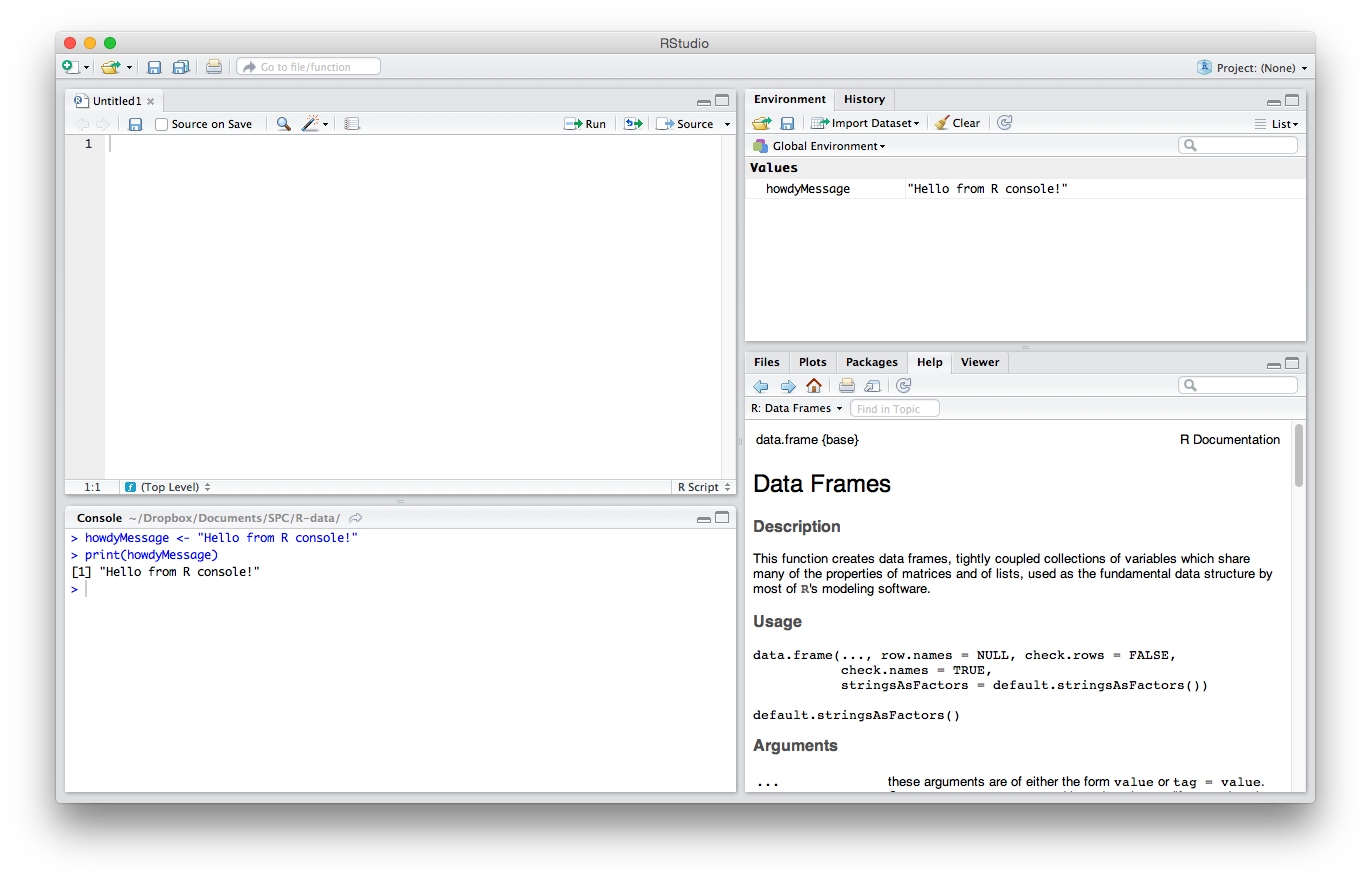
\includegraphics[width=650px]{images/rstudio} \caption{RStudio Window}\label{fig:rstudio}
\end{figure}

\subsubsection{The RStudio Interface}\label{the-rstudio-interface}

If you open RStudio, you get a window which look like Figure \ref{fig:rstudio}. RStudio has

\begin{itemize}
\tightlist
\item
  a console that you will use to enter commands and try out code (appearing as the \textbf{bottom left} window)
\item
  there is a script editor on the \textbf{top left}
\item
  a window with the `'Environment'' tab (\textbf{top right} window), which shows functions and objects you have created and which are currently in memory, and
\item
  a window that shows plots, files packages, and help documentation (\textbf{bottom right})
\end{itemize}

You will learn more how to use this program during this course.

\begin{geek}
If you have already programming experiences and a strong preference for
a certain coding editor or IDE, you may use your preferred coding
environment and integrate the \emph{R} command line software to run your
scripts.

Using coding editors is never as comfortable as working with the
specialized tool \emph{RStudio}. However, some nerds want the puristic
command line experiences.
\end{geek}

\subsection{Code examples}\label{code-examples}

The manual comprises many code examples. A code example always looks like this:

\begin{Shaded}
\begin{Highlighting}[]
\DecValTok{7} \SpecialCharTok{+} \DecValTok{8}
\end{Highlighting}
\end{Shaded}

The output that \emph{R} returns in the console after processing the command is indicated in the manual with \texttt{\#\#} and looks like this:

\begin{verbatim}
## [1] 15
\end{verbatim}

It is suggest to execute the code examples in your own \emph{R}-console and see what the results are. To do so, copy \& paste the code in the console and press enter. \emph{R} executes the code and give you feedback. In RStudio it like this:

\begin{center}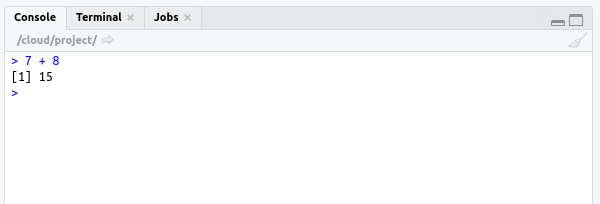
\includegraphics[width=450px]{images/console} \end{center}

\emph{Hint}: You can copy the code examples from the online manual by the clicking on the `copy-button', which appears if you move with the mouse course to right-top corner of the code example field.

\begin{center}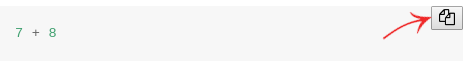
\includegraphics[width=450px]{images/click_copy_code} \end{center}

\subsubsection{Text boxes}\label{text-boxes}

There are different types of text boxes:

\begin{important}
\textbf{Important} information.
\end{important}

\begin{geek}
Additional information for \textbf{advanced learners}. This is only for
nerds and not relevant for most students. If you want, can simply
ignored it.
\end{geek}

\begin{myexercise}
This icon indicates an \textbf{exercise}. Solutions to some exercise
problems are provided and help to check whether you understood the
learning material. In the online version the solutions are hidden and
will be display only on request.
\end{myexercise}
\webexhide{Solution}

\begin{Shaded}
\begin{Highlighting}[]
\CommentTok{\# This is a solution to an exercise problem.}
\end{Highlighting}
\end{Shaded}

\webexunhide

\subsection{Trial-and-error learning}\label{trial-and-error-learning}

Trial-and-error is very essential for learning to program. I therefore suggest: \emph{Play around with the code examples and see happens if you change them.}

You will face many error and warning messages as a consequence. But that fine! Learning to understand error messages is, in my view, the key to learn to program. Thus, read the error messages always carefully (instead of freaking out) and try to figure out what the origin of this underlying error is. This is not always easy and finding a bug in a program code (called \emph{debugging}) is often very time-consuming. However, it is an important (if not the most important) skill for any data scientist.

Don't worry, if you have the feeling at the beginning that you spend most of your time with debugging---you have to know, is quite normal.

\section{Finding Help}\label{findinghelp}

Learning to programming means trying things out, change stuff in the code and see what happens. Unfortunately, try-and-error is the only way to became a good data analyst or programmer.

Please note, you will face \textbf{very often} error messages! Don't get scared, \textbf{read the error messages carefully} and try to understand what the cause of the problem is.

There is another type of mistake: Sometimes \emph{R} commands or scripts do not show an error message, but if you look carefully you notice that the \emph{R} doesn't do what you want or reveals very strange and impossible results. Checks therefore the effects of your steps always very carefully. This is can be sometimes a trick situation. Learning to find the mistake (i.e.~the bug) in your code can become very hard. That is, finding and solving this problems in the script (called ``debugging'') is a key skill that you need to develop throughout this course.

\begin{enumerate}
\def\labelenumi{\arabic{enumi}.}
\item
  If you're struggling how a function works, remember the \texttt{?function} command and use this built-in help documentation of \emph{R} and RStudio (see section \ref{builtinhelp}).
\item
  Look at the \hyperref[readings]{suggested readings and online learning resources} in the Appendix \ref{readings}.
\item
  Note, the internet is your best friend while learning to programming (and afterwards).

  \begin{itemize}
  \item
    Sometimes to helps to find pieces of code of other users online to ``\emph{copy \& paste}'' and ``\emph{change \& see what happens}''. For this you can use in a normal web search engine (e.g.~\href{https://duckduckgo.com/}{DuckDuckGo} or \href{http://www.google.com/en}{Google} or other).
  \item
    If you encounter an error message and you do not understand the reasons for this error, it is very help copy \& paste the error message search for it online. You are probably not the first one who had this problem
  \item
    It is also highly recommanded use question-and-answer-sites for programmers. The most prominent examples is here \href{https://stackoverflow.com/questions/tagged/r}{stackoverflow.com}. Just enter \texttt{{[}r{]}} followed by your question and see, if other user have already asked a similar Question.
  \end{itemize}
\item
  \hyperref[cheatsheets]{Cheat sheets} are nice overviews of \emph{R} functions and helpful, if you can't remember correctly how to use the functions. They are however not self-explaining.
\end{enumerate}

\begin{important}
\subsubsection*{Difficulties with the exercises and
assignments}\label{difficulties-with-the-exercises-and-assignments}
\addcontentsline{toc}{subsubsection}{Difficulties with the exercises and
assignments}

If you are having difficulties with the exercises or assignments and you
can not solve the problem yourself, ask your question during the
\textbf{tutorial sessions}. The idea of the tutorial sessions is to
provide hands-on support you need to do the exercises and answer all
your questions. Make use of this sessions.

You might also use the \textbf{Canvas discussions} of this course and
ask others students, which likely stumble over the same issue. If many
students use this course discussion of exchange, I can become a very
productive tool.
\end{important}

\newpage

\part{Basics}\label{part-basics}

\section{Getting started}\label{gettingstarted}

To get started to working with \emph{R} on your own PC or laptop, you have to install \emph{R} and RStudio. Details about how to install it on your computer can be found below and in one of the instruction videos.

\subsection{\texorpdfstring{Installing \emph{R} and \emph{RStudio} on your PC}{Installing R and RStudio on your PC}}\label{installing-r-and-rstudio-on-your-pc}

\begin{myexercise}
\textbf{Install \emph{R}}

Depending on the operating system (OS), download the latest release of
\href{https://cran.rstudio.com/bin/windows/base/}{R for Windows} or
\href{https://cran.rstudio.com/}{R for MacOSX or Linux} and install it.
If you use Linux, you can install the package \texttt{r-base} via your
package manager.
\end{myexercise}

\begin{myexercise}
\textbf{Download \emph{RStudio} and install it.}

Use the correct installer for your operation system from
\href{https://rstudio.com/products/rstudio/download/\#download}{RStudio
homepage}.
\end{myexercise}

If you face problems with the installation you might find \href{https://techvidvan.com/tutorials/install-r/}{Step-by-Step Guide for Installing R and R Studio} useful. However, there are also several other of tutorials onli\{-\}ne.

\subsection{Creating a Project}\label{creating-a-project}

To get started with your own programming in \emph{RStudio} and with this course you need to create a project that you use for all your exercises during this course.

\begin{myexercise}
Open \emph{RStudio} and click in the menu
\texttt{File\ -\ New\ Project},
\texttt{New\ Directory\ -\ New\ Project}, select a directory name
(e.g.~`R-practical') and select a subdirectory, where your want to save
the project. Click \texttt{Create\ Project}.
\end{myexercise}

\textbf{Now, you are ready to started working with \emph{R}\ldots{}}

Even though you can program and edit \emph{R} files without making a \emph{RStudio} project, I \textbf{strongly recommend} to work always within a project. That is, the first you should do, when opening \emph{RStudio} is the check, if you are in the right project or make new project, if you start a new data analysis. By the way, \_RStudio\_\_ automatically opens the last used project.

Why should I use projects? When working with \emph{R}, you are running your program code from a certain \textbf{working directory} (You can change the working directory \href{https://www.youtube.com/watch?v=LNw6hzGgyxM}{like this}.). From this directory you access all your data files and \emph{R} scripts. It's therefore crucial that you have files and data in the correct folder structure and that you are in the right directory. A project saves the last working directory and the state of your previous work. That is very handy.

\section{Basics of Programming in R}\label{basics}

Learning to work with \emph{R} requires a little knowledge about basic concepts of computer programming. This is maybe a bit technical at the beginning. However, having an insight in this basics makes it later much easy to deal with real data analysis in \emph{R} later.

Thus, the section covers the basics of the \emph{R} programming language. If you are already familiar with any another programming language, I guess these things are not new for you.

\subsection{Comments in Program Code}\label{comments-in-program-code}

Before we have a look at the first \emph{R} code examples, you should know that \emph{R} ignores everything that follows a hashtag \texttt{\#}. That is, text after a \texttt{\#} will not be executed. Hashtags are used to add comments to \emph{R}-code. The comments help to document and explains the code and make it thus more readable for humans. Comments in \emph{R} code are printed in italic font and a different color by \emph{RStudio} (and in the manual). See this example:

\begin{Shaded}
\begin{Highlighting}[]
\CommentTok{\# Example of code with comments}
\NormalTok{x }\OtherTok{=}\NormalTok{ a }\SpecialCharTok{/}\NormalTok{ b       }\CommentTok{\# dividing a by b and storing the result in x}
\end{Highlighting}
\end{Shaded}

That is, if you try out the code examples, you can simple ignore the comment.

\begin{important}
If you later develop your own analyses scripts in \emph{R}, it is
\textbf{strongly} suggested to make use of comments. Only well
documented code is readable code. Only if you comment your code, you
will be able to remember after a few days why you did what and how your
codes works.
\end{important}

\subsection{Variables and Objects}\label{variables-and-objects}

Everything that is stored in \emph{R} is called an \textbf{object}. The most basic example for an object is an numerical \textbf{variable}. For instance,

\begin{Shaded}
\begin{Highlighting}[]
\NormalTok{a }\OtherTok{\textless{}{-}} \DecValTok{9}
\NormalTok{b }\OtherTok{\textless{}{-}} \FloatTok{2724.54}
\NormalTok{third\_variable }\OtherTok{\textless{}{-}} \DecValTok{71}
\end{Highlighting}
\end{Shaded}

In this example, the numerical \texttt{9}, \texttt{2724.54} and \texttt{71} are stored in the variables with the names \texttt{a}, \texttt{b} and \texttt{third\_variable}.
If you want to print out the content of a certain object or variable, you can use the \texttt{print()}-command together with the variable.

\begin{Shaded}
\begin{Highlighting}[]
\FunctionTok{print}\NormalTok{(b)}
\end{Highlighting}
\end{Shaded}

\begin{verbatim}
## [1] 2724.54
\end{verbatim}

\(\ldots\) or even simpler, just enter the variable name in the console

\begin{Shaded}
\begin{Highlighting}[]
\NormalTok{third\_variable}
\end{Highlighting}
\end{Shaded}

\begin{verbatim}
## [1] 71
\end{verbatim}

\begin{simple}
This \href{https://vimeo.com/220493412}{video} also explains objects in
\emph{R}.
\end{simple}

\subsubsection{Variable Environment}\label{variable-environment}

All variables are sorted in the data workspace or environment. In RStudio, you can find the current content of the workspace with all variables the right top panel called ``environment''.

Alternatively, the command \texttt{ls()} lists all objects variables in the R console.

\begin{Shaded}
\begin{Highlighting}[]
\FunctionTok{ls}\NormalTok{()}
\end{Highlighting}
\end{Shaded}

\begin{verbatim}
## [1] "a"              "b"              "hide"           "is_latex"      
## [5] "third_variable" "unhide"
\end{verbatim}

\subsubsection{\texorpdfstring{Equal Sign Assignments (\texttt{=})}{Equal Sign Assignments (=)}}\label{assign}

As you have see above, to assign a value to an object (i.e., variable) with the left arrow \texttt{\textless{}-}. In RStudio, the shortcut \texttt{alt\ \&\ -} is very handy for quickly typing this sign. Check it out.

Instead of typing an left arrow \texttt{\textless{}-} you can use the equal sign \texttt{=}. This two comments have the identical effect:

\begin{Shaded}
\begin{Highlighting}[]
\NormalTok{x }\OtherTok{\textless{}{-}} \DecValTok{13}
\NormalTok{x }\OtherTok{=} \DecValTok{13}
\end{Highlighting}
\end{Shaded}

Many data scientists find the equal-sign syntax easier to type and more natural to read. If you also prefer using \texttt{=} instead of \texttt{\textless{}-}, just do it. It's not a problem.

You just need to know, that the coding style guidelines in the \emph{R} community suggest to use the \texttt{\textless{}-} syntax. (see e.g.~\href{https://www.r-bloggers.com/why-do-we-use-arrow-as-an-assignment-operator/}{here} for reasons). Most examples and documentations that you find online use therefore the arrow as the assignment operator.

To avoid any confusion, the current manual uses the \texttt{\textless{}-} operator .

\subsubsection{Left and Right Hand Side Assignments}\label{left-and-right-hand-side-assignments}

In \emph{R}, there are two different ways to assign a value to a variable; you can either assign from left to right or from right to left in R. That is, instead of using \texttt{\textless{}-} or \texttt{=}to assign a value to a variable (left-hand-side assignment), you can also work with so-called the right-hand-side assignments (\texttt{-\textgreater{}}). These comments illustrate the principle:

\begin{Shaded}
\begin{Highlighting}[]
\NormalTok{x }\OtherTok{\textless{}{-}} \DecValTok{13}       \CommentTok{\# left{-}hand{-}side assignment}
\DecValTok{13} \OtherTok{{-}\textgreater{}}\NormalTok{ x       }\CommentTok{\# right{-}hand{-}side assignment}

\NormalTok{a }\OtherTok{\textless{}{-}}\NormalTok{ b        }\CommentTok{\# a receives the value of b}
\NormalTok{a }\OtherTok{{-}\textgreater{}}\NormalTok{ b        }\CommentTok{\# b receives the value of a}
\end{Highlighting}
\end{Shaded}

Left-hand-side assignments are most common among users, because the are similar of what we are used to in mathematical equations. You will see later in the course (when working with \textbf{pipes}), why right-hand-side assignment can be very elegant and efficient for data science.

\begin{myexercise}
What happens in the command below? What are the changes variable
environment?

\texttt{E\ =\ U\ =\ R\ =\ 2}
\end{myexercise}
\webexhide{Solution}

\begin{Shaded}
\begin{Highlighting}[]
\CommentTok{\# 1. The value 2 is assigned to R.}
\CommentTok{\# 2. U is assigned to R}
\CommentTok{\# 3. E is assigned to U}
\CommentTok{\# That is, you have three variables with the value 2}
\end{Highlighting}
\end{Shaded}

\webexunhide

\subsection{Basic operations}\label{basic-operations}

You use \emph{R} as a calculator and perform basic operations on numbers and variables numbers. Just enter the following examples the console and check the results:

\begin{Shaded}
\begin{Highlighting}[]
\NormalTok{a }\OtherTok{\textless{}{-}} \DecValTok{8}

\DecValTok{12} \SpecialCharTok{+} \DecValTok{6}
\NormalTok{a }\SpecialCharTok{*} \DecValTok{2}
\DecValTok{210} \SpecialCharTok{/} \DecValTok{3}
\NormalTok{(a }\SpecialCharTok{{-}} \DecValTok{3}\NormalTok{) }\SpecialCharTok{/} \DecValTok{4}
\DecValTok{4}\SpecialCharTok{**}\DecValTok{3}     \CommentTok{\# 4 to the power of 5}
\end{Highlighting}
\end{Shaded}

Of course, the result of a calculations can be stored in new variables, for instance:

\begin{Shaded}
\begin{Highlighting}[]
\NormalTok{x }\OtherTok{\textless{}{-}}\NormalTok{ a }\SpecialCharTok{*} \DecValTok{7}
\NormalTok{x}
\end{Highlighting}
\end{Shaded}

\begin{verbatim}
## [1] 63
\end{verbatim}

Look at the following example, which increases the value of the variable \texttt{x} by 1. To do so, it stores the result of the operation \texttt{x\ +\ 1} again in \texttt{x}:

\begin{Shaded}
\begin{Highlighting}[]
\NormalTok{x }\OtherTok{\textless{}{-}} \DecValTok{9}
\NormalTok{x }\OtherTok{\textless{}{-}}\NormalTok{ x }\SpecialCharTok{+} \DecValTok{1}
\NormalTok{x}
\end{Highlighting}
\end{Shaded}

\begin{verbatim}
## [1] 10
\end{verbatim}

\begin{myexercise}
See the code example below. If \texttt{r} represents the radius of a
circle, what is \texttt{x} ?
\end{myexercise}

\begin{Shaded}
\begin{Highlighting}[]
\NormalTok{r }\OtherTok{=} \DecValTok{19}
\NormalTok{pi}\SpecialCharTok{*}\NormalTok{(r}\SpecialCharTok{**}\DecValTok{2}\NormalTok{) }\OtherTok{{-}\textgreater{}}\NormalTok{ x}
\end{Highlighting}
\end{Shaded}

\webexhide{Solution}

\begin{Shaded}
\begin{Highlighting}[]
\CommentTok{\# The area, which is pi times radius squared.}
\end{Highlighting}
\end{Shaded}

\webexunhide

\subsection{Non-numerical data types}\label{non-numerical-data-types}

\subsubsection{Character}\label{character}

Besides numeric values as in the example above, \emph{R} can store text (called \texttt{character}) in variables.

\begin{Shaded}
\begin{Highlighting}[]
\NormalTok{txt }\OtherTok{\textless{}{-}} \StringTok{"Erasmus"}
\end{Highlighting}
\end{Shaded}

You can see the new variable in the current workspace (see `'environment''-panel).

Certain operations can be only performed with certain data types. For instance,
it does not make sense to substract or add to text string, right? See what happens:

\begin{Shaded}
\begin{Highlighting}[]
\NormalTok{a }\OtherTok{\textless{}{-}} \StringTok{"Hello"}
\NormalTok{b }\OtherTok{\textless{}{-}} \StringTok{"World"}
\end{Highlighting}
\end{Shaded}

\begin{Shaded}
\begin{Highlighting}[]
\NormalTok{a }\SpecialCharTok{+}\NormalTok{ b}
\end{Highlighting}
\end{Shaded}

\begin{verbatim}
## Error in a + b : non-numeric argument to binary operator
\end{verbatim}

If you want to concatenate two strings you have to use the function \texttt{paste}:

\begin{Shaded}
\begin{Highlighting}[]
\FunctionTok{paste}\NormalTok{(a, b)}
\end{Highlighting}
\end{Shaded}

\begin{verbatim}
## [1] "Hello World"
\end{verbatim}

\begin{important}
\emph{R} can sometimes convert one atomic data type into another data
type. Function that convert data types start in \emph{R} with
``\texttt{as.}''. For instance,

\begin{itemize}
\tightlist
\item
  \texttt{as.character()} converts as numbers into a string
\item
  \texttt{as.numeric()} converts a character into number. see section
  \ref{comparediffdata}
\end{itemize}
\end{important}

\subsubsection{Logicals}\label{logicals}

Another often reoccurring data type is call \emph{logical} (in other programming languages it's other call \emph{boolean}). A logical can be only \texttt{TRUE} or \texttt{FALSE} (typed in capitals without quotation marks); it is in other words a binary variable.

Logicals are very important, because are returned by \emph{R} if you make a comparison of the numbers (see section \ref{comparing}.)

\paragraph*{\texorpdfstring{Negation: \texttt{!}}{Negation: !}}\label{negation}
\addcontentsline{toc}{paragraph}{Negation: \texttt{!}}

In \emph{R}, \texttt{!} is used for the negation of logicals and reads like ``\emph{is not}''. It converts, in other words, a \texttt{TRUE} to \texttt{FALSE} and \texttt{FALSE} to \texttt{TRUE}:

\begin{Shaded}
\begin{Highlighting}[]
\SpecialCharTok{!}\ConstantTok{TRUE}    \CommentTok{\#  reads like "is not true"}
\end{Highlighting}
\end{Shaded}

\begin{verbatim}
## [1] FALSE
\end{verbatim}

\begin{Shaded}
\begin{Highlighting}[]
\SpecialCharTok{!}\ConstantTok{FALSE}   \CommentTok{\#  reads like "is not false"}
\end{Highlighting}
\end{Shaded}

\begin{verbatim}
## [1] TRUE
\end{verbatim}

\subsubsection{Combining different data types}\label{comparediffdata}

Please note, that you can preform the same operation that not combing a numerical and text variable is, of course, not possible. Try what happens if you type:

\begin{Shaded}
\begin{Highlighting}[]
\NormalTok{a }\OtherTok{\textless{}{-}} \DecValTok{4}
\NormalTok{b }\OtherTok{\textless{}{-}} \StringTok{"12"}
\NormalTok{a }\SpecialCharTok{*}\NormalTok{ b}
\end{Highlighting}
\end{Shaded}

The third line results in an error, because \texttt{a} is a number and \texttt{b} is a text object. Combining this different data types is not possible, because \emph{R} does not know what to do.

\begin{myexercise}
Why does this work?

\texttt{a\ *\ as.numeric(b)}
\end{myexercise}
\webexhide{Solution}

\begin{Shaded}
\begin{Highlighting}[]
\CommentTok{\# b is a string, but it will be converted to a number (by the function}
\CommentTok{\# as.numeric). Multiplying two number is, of course, a valid operation.}
\end{Highlighting}
\end{Shaded}

\webexunhide

rite the R code for the following equation:

\subsection{Comparing values}\label{comparing}

You can compare numerical variables using comparators. For example,

\begin{Shaded}
\begin{Highlighting}[]
\NormalTok{a }\OtherTok{\textless{}{-}} \DecValTok{27}
\NormalTok{b }\OtherTok{\textless{}{-}} \DecValTok{30}
\NormalTok{a }\SpecialCharTok{\textgreater{}}\NormalTok{ b}
\end{Highlighting}
\end{Shaded}

\begin{verbatim}
## [1] FALSE
\end{verbatim}

You see that this expression is incorrect, because \(27<30\) .

Further comparisons are:

\begin{Shaded}
\begin{Highlighting}[]
\NormalTok{a }\SpecialCharTok{\textless{}}\NormalTok{ b}
\NormalTok{a }\SpecialCharTok{==}\NormalTok{ b   }\CommentTok{\# Are a and b are equal?}
\NormalTok{a }\SpecialCharTok{!=}\NormalTok{ b   }\CommentTok{\# Is a unequal to b?}
\end{Highlighting}
\end{Shaded}

Note that \emph{R} needs two equal signs \texttt{==} for an `'is-equal-comparison''. One equal sign is interpreted by \emph{R} as an assignment, similar to \texttt{\textless{}-} (see section \ref{assign}).

\subsection{Functions}\label{functions}

As other programming languages, \emph{R} has \textbf{functions} to perform a specific tasks in a program, for instance, to process or manipulate data. A function ``returns'' a results of the command or the processing. For instance, the function \texttt{ls()} lists current variables in the workspace.

\begin{important}
To execute a function, you always have call the function name
\textbf{followed by parentheses}.

Forgetting the parentheses results in strange behaviour. (That is,
\emph{R} displays the definition of the function, if you just entering
the function name.)
\end{important}

\subsubsection{Arguments}\label{arguments}

Often, functions take one or more arguments. The arguments are for instance data to be processed or certain information that are required to execute the task. For instance,

\begin{Shaded}
\begin{Highlighting}[]
\FunctionTok{log}\NormalTok{(}\DecValTok{64}\NormalTok{)}
\end{Highlighting}
\end{Shaded}

\begin{verbatim}
## [1] 4.158883
\end{verbatim}

returns the logarithm natural of 13, \(\log_e(13)\), and prints it out in the RStudio console. You can also save the result directly in another variable, because you want to do some further processing later with it or you can combine functions. For example:

\begin{Shaded}
\begin{Highlighting}[]
\NormalTok{x }\OtherTok{\textless{}{-}} \FunctionTok{log}\NormalTok{(}\DecValTok{64}\NormalTok{)}
\end{Highlighting}
\end{Shaded}

\begin{simple}
\href{https://vimeo.com/220490105}{See also this video explaining
functions in \emph{R}.}
\end{simple}

You can also feed the result of a function directly into another function. For example:

\begin{Shaded}
\begin{Highlighting}[]
\FunctionTok{sqrt}\NormalTok{(}\FunctionTok{log}\NormalTok{(}\DecValTok{64}\NormalTok{))}
\end{Highlighting}
\end{Shaded}

\texttt{sqrt()} is the command for the square root. This nesting of functions and expressions makes it the implement mathematical expression in \emph{R} very straightforward. For instance, is

\begin{myexercise}
Write the R code for the following equation:

\[x = \sqrt{15^\frac{\log_e(12)}{1+ \sin(4.5 \pi)}}\]

Hint: \texttt{sin()} is function for sinus. The variable \texttt{pi} is
always predefine in R, even if you can not see it in the environment
panel.
\end{myexercise}
\webexhide{Solution}

\begin{Shaded}
\begin{Highlighting}[]
\NormalTok{x }\OtherTok{\textless{}{-}} \FunctionTok{sqrt}\NormalTok{(}\DecValTok{15}\SpecialCharTok{**}\FunctionTok{log}\NormalTok{(}\DecValTok{12}\NormalTok{) }\SpecialCharTok{/} \DecValTok{1} \SpecialCharTok{+} \FunctionTok{sin}\NormalTok{(}\FloatTok{4.5}\SpecialCharTok{*}\NormalTok{pi))}
\CommentTok{\# Sorry, I know the example is not a very meaningful.}
\end{Highlighting}
\end{Shaded}

\webexunhide

Importantly: Functions expect a specific data type as argument. If the type of the argument is not correct, you will receive an error. For instance, the function \texttt{sin()} (the sinus) expects a number not a text string. Look what happens:

\begin{Shaded}
\begin{Highlighting}[]
\NormalTok{x }\OtherTok{=} \StringTok{"1987"}
\FunctionTok{sin}\NormalTok{(x)}
\end{Highlighting}
\end{Shaded}

\textbf{Required and optional arguments}

Some arguments of functions are required (that is, you have to specify this them) and others are optional. Optional arguments will often use a default value (normally specified in the help documentation), if you do not enter any value.

For instance, if you just call \texttt{log(64)} you get the natural logarithm \(\log_e(64)\). If you want to have the logarithm to a different base, e.g.~\(\log_{2}\) or \(\log_{10}\), you have to specify the optional argument \texttt{base} of the \texttt{log} function:

\begin{Shaded}
\begin{Highlighting}[]
\FunctionTok{log}\NormalTok{(}\DecValTok{64}\NormalTok{, }\AttributeTok{base=}\DecValTok{2}\NormalTok{)}
\end{Highlighting}
\end{Shaded}

\begin{verbatim}
## [1] 6
\end{verbatim}

\begin{Shaded}
\begin{Highlighting}[]
\FunctionTok{log}\NormalTok{(}\DecValTok{64}\NormalTok{, }\AttributeTok{base=}\DecValTok{10}\NormalTok{)}
\end{Highlighting}
\end{Shaded}

\begin{verbatim}
## [1] 1.80618
\end{verbatim}

\subsubsection{Built-in help for functions}\label{builtinhelp}

\emph{R} provides hundreds functions. As you will see late in section \ref{packages}, you can install additional packages for specific tasks, which provide basically collections of extra functions. That is, the amount of functions that you can use in \emph{R} is almost endless.

But how do you know what a specific functions is doing and which arguments you can or have to define to use it correctly. Fortunately, \emph{R} has a \textbf{built-in help system}. You can look up all the arguments that a function takes by using the help documentation by using the format ``\texttt{?function}''.

As an example, let's look at the help documentation for the function \texttt{rnorm()} which randomly generates a set of numbers with a normal distribution.

\subsubsection{Example}\label{examplernorm}

Display the documentation of the function \texttt{rnorm} by typing

\begin{Shaded}
\begin{Highlighting}[]
\NormalTok{?rnom}
\end{Highlighting}
\end{Shaded}

The help documentation should appear in the bottom right panel. In the usage section of the documentation, we see that \texttt{rnorm()} takes the following form:

\begin{itemize}
\tightlist
\item
  \texttt{rnorm(n,\ mean\ =\ 0,\ sd\ =\ 1)}
\end{itemize}

In the arguments section, there are explanations for each of the arguments. \texttt{n} is the number of random numbers we want to create, \texttt{mean} is the mean of the data points we will create and \texttt{sd} is the standard deviation of the set. In the details section it notes that if no values are entered for \texttt{mean} and \texttt{sd} it will use a default of 0 and 1 for these values. Because there is no default value for \texttt{n} it must be specified otherwise the code won't run.

Let's try an example and just change the required argument \texttt{n} to ask \emph{R} to produce 5 random numbers.

\begin{Shaded}
\begin{Highlighting}[]
\FunctionTok{rnorm}\NormalTok{(}\AttributeTok{n =} \DecValTok{5}\NormalTok{)}
\end{Highlighting}
\end{Shaded}

\begin{verbatim}
## [1] -1.6176612 -0.3687978  0.1028284 -1.0116232 -0.9252869
\end{verbatim}

The random numbers have a mean of 0 and an SD of 1. Of course, since this are random numbers, you have probably got different numbers. Run the function again and you will see that you get each time different `'random'' numbers.

Now we can change the additional arguments to produce a different set of numbers.

\begin{Shaded}
\begin{Highlighting}[]
\FunctionTok{rnorm}\NormalTok{(}\AttributeTok{n =} \DecValTok{5}\NormalTok{, }\AttributeTok{mean =} \DecValTok{100}\NormalTok{, }\AttributeTok{sd =} \DecValTok{15}\NormalTok{)}
\end{Highlighting}
\end{Shaded}

\begin{verbatim}
## [1]  78.90288 112.93548  73.47952  83.67293  74.85587
\end{verbatim}

This time \emph{R} has still produced 5 random numbers, but now this set of numbers has a mean of 100 and a standard deviation of 15 as specified (this is the distribution of the scores in many IQ tests). Always remember to use the help documentation to help you understand what arguments a function requires.

\subsubsection{Argument names}\label{argument-names}

In the above examples, we have written out the argument names in our code (e.g., \texttt{n}, \texttt{mean}, \texttt{sd}), however, this is not strictly necessary. The following two lines of code would both produce the same result (although each time you run \texttt{rnorm()} it will produce a slightly different set of numbers, because it's random, but they would still have the same mean and SD):

\begin{Shaded}
\begin{Highlighting}[]
\FunctionTok{rnorm}\NormalTok{(}\AttributeTok{n =} \DecValTok{7}\NormalTok{, }\AttributeTok{mean =} \DecValTok{10}\NormalTok{, }\AttributeTok{sd =} \DecValTok{2}\NormalTok{)}
\FunctionTok{rnorm}\NormalTok{(}\DecValTok{7}\NormalTok{, }\DecValTok{10}\NormalTok{, }\DecValTok{2}\NormalTok{)}
\end{Highlighting}
\end{Shaded}

Importantly, if you do not write out the argument names, R will use the default order of arguments, that is for \texttt{rnorm} it will assume that the first number you enter is \texttt{n}. the second number is mean and the third number is \texttt{sd}.

If you write out the argument names then you can write the arguments in whatever order you like:

\begin{Shaded}
\begin{Highlighting}[]
\FunctionTok{rnorm}\NormalTok{(}\AttributeTok{sd =} \DecValTok{2}\NormalTok{, }\AttributeTok{n =} \DecValTok{7}\NormalTok{, }\AttributeTok{mean =} \DecValTok{10}\NormalTok{)}
\end{Highlighting}
\end{Shaded}

When you are first learning R, you may find it useful to write out the argument names as it can help you remember and understand what each part of the function is doing. However, as your skills progress you may find it quicker to omit the argument names and you will also see examples of code online that do not use argument names so it is important to be able to understand which argument each bit of code is referring to (or look up the help documentation to check).

In this manual, I will mostly write out the argument names the first time , however, in subsequent uses they may be omitted.

\begin{important}
The assign a value to an named argument of the function, you have to use
the equal sign \texttt{=} and not \texttt{\textless{}-}.
\end{important}

\subsubsection{Tab auto-complete}\label{tab-auto-complete}

One very useful feature of R Studio is the tab auto-complete for functions (see Figure \ref{fig:autocomplete}). If you write the name of the function and then press the tab key, R Studio will show you the arguments that function takes along with a brief description. If you press enter on the argument name it will fill in the name for you, just like auto-complete on your phone. This is incredibly useful when you are first learning R and you should remember to use this feature frequently.

\begin{figure}
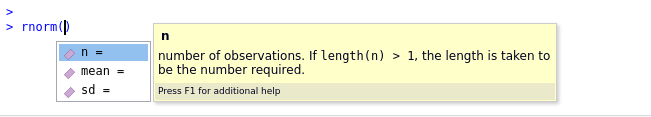
\includegraphics[width=450px]{images/autocomplete} \caption{The tab auto-complete of RStudio.}\label{fig:autocomplete}
\end{figure}

\begin{myexercise}
Get the documentation of the optional argument \texttt{sd} via the
autocomplete function in RStudio. Compare it with the
\texttt{?}-documentation.
\end{myexercise}

\subsubsection{Important Base R functions}\label{important-base-r-functions}

When you install \emph{R} you will have access to a range of functions including options for data wrangling and statistical analysis. These functions that are included in the default installation are typically referred to as Base \emph{R} . There is a very useful overview that shows the most important Base \emph{R} functions.

An overview of this functions is online available as pdf and call the ``\hyperref[cheatsheets]{Base R cheat sheet}''.

Don't worry, you don't have to know this functions. You just have to know \textbf{how to figure out} which function is needed to accomplish you task and where you find to detailed information how to use this function (see section \ref{findinghelp}).

\subsubsection{User-defined functions}\label{user-defined-functions}

The real power of a programming language is that you can develop your own functions that accomplish reoccurring tasks or that this way facilitate or structures your analysis.

Moreover, there are many collections of additional functions for specific tasks available online. They extend your \emph{R} functionality and have been programmed by other data analysts or statisticians. This extensions are called in \emph{R} ``\textbf{packages}''.

Later in the course we will a package called \href{https://www.tidyverse.org/}{Tidyverse}, which extends the \emph{R} by many convenient functions for data handling. But for know, let's keep it simple and just focus for now on the usages of the basic built-in functions in \emph{R}.

\begin{geek}
If you want to develop your own functions (or even packages), please
have a look, for instance, at the
\href{https://r4ds.had.co.nz/functions.html}{online tutorial} of
Grolemund and Wickham or see the \hyperref[readings]{suggested reading}.
\end{geek}

\newpage

\part{Data Structures}\label{part-data-structures}

\section{Atomic Vectors}\label{vectors}

A dataset consists typically not only of a single number or a single data point. We need to be able to deal with collections of data points or datasets. \emph{R} knows different types of objects that store datasets.

We'll start with the most basics type of data structure in \emph{R} , which is an \textbf{atomic vector}. A vector is merely a list of data points. They are very simple and they do show up everywhere. If you look closely enough, you'll see later that almost all data structures in \emph{R} are built from atomic vectors.

You can make an atomic vector by grouping some values of data together with the command \texttt{c()} (which stands for concatenate).

\begin{Shaded}
\begin{Highlighting}[]
\NormalTok{vec }\OtherTok{\textless{}{-}} \FunctionTok{c}\NormalTok{(}\DecValTok{1}\NormalTok{,}\DecValTok{2}\NormalTok{,}\DecValTok{3}\NormalTok{,}\DecValTok{4}\NormalTok{,}\DecValTok{5}\NormalTok{,}\DecValTok{6}\NormalTok{)}
\NormalTok{vec}
\end{Highlighting}
\end{Shaded}

\begin{verbatim}
## [1] 1 2 3 4 5 6
\end{verbatim}

\begin{Shaded}
\begin{Highlighting}[]
\NormalTok{vector\_of\_logicals  }\OtherTok{\textless{}{-}} \FunctionTok{c}\NormalTok{(}\ConstantTok{FALSE}\NormalTok{, }\ConstantTok{TRUE}\NormalTok{, }\ConstantTok{TRUE}\NormalTok{, }\ConstantTok{FALSE}\NormalTok{)}
\NormalTok{vector\_of\_logicals}
\end{Highlighting}
\end{Shaded}

\begin{verbatim}
## [1] FALSE  TRUE  TRUE FALSE
\end{verbatim}

\begin{Shaded}
\begin{Highlighting}[]
\NormalTok{days\_of\_week }\OtherTok{\textless{}{-}} \FunctionTok{c}\NormalTok{(}\StringTok{"Monday"}\NormalTok{, }\StringTok{"Tuesday"}\NormalTok{, }\StringTok{"Wednesday"}\NormalTok{, }\StringTok{"Thursday"}\NormalTok{, }\StringTok{"Friday"}\NormalTok{,}
                \StringTok{"Saturday"}\NormalTok{, }\StringTok{"Sunday"}\NormalTok{)}
\NormalTok{days\_of\_week}
\end{Highlighting}
\end{Shaded}

\begin{verbatim}
## [1] "Monday"    "Tuesday"   "Wednesday" "Thursday"  "Friday"    "Saturday" 
## [7] "Sunday"
\end{verbatim}

You can make vectors of any type of data, but \textbf{one atomic vector comprises only data of one type}! That is, each atomic vector stores its values as a one-dimensional vector, and each atomic vector can only store one data type. If you mix numbers (\emph{integer}, \emph{doubles}), \emph{logicals}, and text (\emph{chanraters}), \emph{R} converts them to one data type. This should be always avoided, because it will cause problems later once you want to calculate with the data.

\begin{Shaded}
\begin{Highlighting}[]
\NormalTok{x }\OtherTok{\textless{}{-}} \FunctionTok{c}\NormalTok{(}\StringTok{"a"}\NormalTok{, }\DecValTok{3}\NormalTok{, }\StringTok{"c"}\NormalTok{, }\FloatTok{6.5}\NormalTok{)}
\NormalTok{x}
\end{Highlighting}
\end{Shaded}

\begin{verbatim}
## [1] "a"   "3"   "c"   "6.5"
\end{verbatim}

As you see, all elements have been converted to character. That's bad. If you want to mix different data types in one collection, you have to use \texttt{list()} as described in chapter \ref{lists}.

\subsubsection*{Concatenating two vectors}\label{concatenating-two-vectors}
\addcontentsline{toc}{subsubsection}{Concatenating two vectors}

You can use the \texttt{c()}-command also to concatenate two vectors:

\begin{Shaded}
\begin{Highlighting}[]
\NormalTok{x }\OtherTok{\textless{}{-}} \FunctionTok{c}\NormalTok{(}\DecValTok{1}\NormalTok{,}\DecValTok{2}\NormalTok{,}\DecValTok{3}\NormalTok{,}\DecValTok{4}\NormalTok{,}\DecValTok{5}\NormalTok{,}\DecValTok{6}\NormalTok{)}
\NormalTok{y }\OtherTok{\textless{}{-}} \FunctionTok{c}\NormalTok{(}\DecValTok{20}\NormalTok{,}\DecValTok{30}\NormalTok{,}\DecValTok{40}\NormalTok{)}
\NormalTok{z }\OtherTok{\textless{}{-}} \FunctionTok{c}\NormalTok{(x, y)}
\NormalTok{z}
\end{Highlighting}
\end{Shaded}

\begin{verbatim}
## [1]  1  2  3  4  5  6 20 30 40
\end{verbatim}

\subsubsection*{Vector length}\label{vector-length}
\addcontentsline{toc}{subsubsection}{Vector length}

The command \texttt{length} returns the number of elements in an atomic vector.

\begin{Shaded}
\begin{Highlighting}[]
\FunctionTok{length}\NormalTok{(days\_of\_week)}
\end{Highlighting}
\end{Shaded}

\begin{verbatim}
## [1] 7
\end{verbatim}

\subsection{Number sequences}\label{number-sequences}

You can generate a simple ascending or descending sequence of integer numbers like this:

\begin{Shaded}
\begin{Highlighting}[]
\NormalTok{x }\OtherTok{\textless{}{-}} \DecValTok{1}\SpecialCharTok{:}\DecValTok{100}   \CommentTok{\# ascending sequence}
\NormalTok{x}
\end{Highlighting}
\end{Shaded}

\begin{verbatim}
##   [1]   1   2   3   4   5   6   7   8   9  10  11  12  13  14  15  16  17  18
##  [19]  19  20  21  22  23  24  25  26  27  28  29  30  31  32  33  34  35  36
##  [37]  37  38  39  40  41  42  43  44  45  46  47  48  49  50  51  52  53  54
##  [55]  55  56  57  58  59  60  61  62  63  64  65  66  67  68  69  70  71  72
##  [73]  73  74  75  76  77  78  79  80  81  82  83  84  85  86  87  88  89  90
##  [91]  91  92  93  94  95  96  97  98  99 100
\end{verbatim}

\begin{Shaded}
\begin{Highlighting}[]
\NormalTok{y }\OtherTok{\textless{}{-}} \DecValTok{49}\SpecialCharTok{:{-}}\DecValTok{50}  \CommentTok{\# descending sequence}
\NormalTok{y}
\end{Highlighting}
\end{Shaded}

\begin{verbatim}
##   [1]  49  48  47  46  45  44  43  42  41  40  39  38  37  36  35  34  33  32
##  [19]  31  30  29  28  27  26  25  24  23  22  21  20  19  18  17  16  15  14
##  [37]  13  12  11  10   9   8   7   6   5   4   3   2   1   0  -1  -2  -3  -4
##  [55]  -5  -6  -7  -8  -9 -10 -11 -12 -13 -14 -15 -16 -17 -18 -19 -20 -21 -22
##  [73] -23 -24 -25 -26 -27 -28 -29 -30 -31 -32 -33 -34 -35 -36 -37 -38 -39 -40
##  [91] -41 -42 -43 -44 -45 -46 -47 -48 -49 -50
\end{verbatim}

What does the numbers in brackets in the output mean? \emph{R} indicates before each output line the position of the next printed element in the vector (e.g.~\texttt{{[}19{]}}). That's why the console output of vectors always start with \texttt{\#\#\ {[}1{]}}.

\subsubsection{Sequence generating functions}\label{sequence-generating-functions}

\emph{R} come with a lot of methods that generate sequence. For instance, for instance the function \texttt{seq()} has be already used in the previous assignment. Let's have a look at some further features of the function. You can also produce floating points with \texttt{seq()}:

\begin{Shaded}
\begin{Highlighting}[]
\FunctionTok{seq}\NormalTok{(}\DecValTok{10}\NormalTok{, }\DecValTok{12}\NormalTok{, }\AttributeTok{by=}\NormalTok{.}\DecValTok{2}\NormalTok{)}
\end{Highlighting}
\end{Shaded}

\begin{verbatim}
##  [1] 10.0 10.2 10.4 10.6 10.8 11.0 11.2 11.4 11.6 11.8 12.0
\end{verbatim}

If you want to make a vector of a particular length (with equalled spaced numbers) you can you the optional argument \texttt{length}. For example,

\begin{Shaded}
\begin{Highlighting}[]
\FunctionTok{seq}\NormalTok{(}\DecValTok{0}\NormalTok{,}\DecValTok{1}\NormalTok{, }\AttributeTok{length=}\DecValTok{12}\NormalTok{) }\CommentTok{\# 12 numbers between 0  and 1}
\end{Highlighting}
\end{Shaded}

\begin{verbatim}
##  [1] 0.00000000 0.09090909 0.18181818 0.27272727 0.36363636 0.45454545
##  [7] 0.54545455 0.63636364 0.72727273 0.81818182 0.90909091 1.00000000
\end{verbatim}

\textbf{Random numbers}

Random numbers sequences are very useful to illustrate probabilistic phenomena in statistics and are required in psychology for mathematical modelling and simulations. \emph{R} can generate random numbers from different probability functions.

Drawing random numbers from a normal distribution has already been discussed in section \ref{examplernorm}. The function \texttt{runif()} is used draw random numbers from a uniform distribution:

\begin{Shaded}
\begin{Highlighting}[]
\FunctionTok{runif}\NormalTok{(}\DecValTok{10}\NormalTok{)                     }\CommentTok{\# 10 random numbers between 0 and 1}
\end{Highlighting}
\end{Shaded}

\begin{verbatim}
##  [1] 0.09508382 0.54582978 0.22742061 0.34666212 0.95768098 0.81936021
##  [7] 0.34899394 0.19600054 0.24845279 0.90685759
\end{verbatim}

\begin{Shaded}
\begin{Highlighting}[]
\FunctionTok{runif}\NormalTok{(}\DecValTok{10}\NormalTok{, }\AttributeTok{min=} \DecValTok{10}\NormalTok{, }\AttributeTok{max =} \DecValTok{99}\NormalTok{)  }\CommentTok{\# 10 random numbers between 10 and 99}
\end{Highlighting}
\end{Shaded}

\begin{verbatim}
##  [1] 77.69987 88.94767 49.27783 20.49960 87.80350 50.08093 71.10294 59.51867
##  [9] 21.47696 70.33902
\end{verbatim}

\begin{geek}
More information about random number generation and the probability
distributions that are implemented in base \emph{R} can be found by
calling \texttt{?RNG} and \texttt{?distributions}.
\end{geek}

\subsection{Manipulating vectors}\label{manipulating-vectors}

If you apply an operation on a vector, \emph{R} applies it to each element. You have seen already some examples.

\webexhide{Some examples}

\begin{Shaded}
\begin{Highlighting}[]
\NormalTok{v }\OtherTok{\textless{}{-}} \FunctionTok{c}\NormalTok{(}\DecValTok{1}\NormalTok{,}\DecValTok{2}\NormalTok{,}\DecValTok{3}\NormalTok{,}\DecValTok{4}\NormalTok{,}\DecValTok{5}\NormalTok{,}\DecValTok{6}\NormalTok{)}
\NormalTok{v }\SpecialCharTok{+} \DecValTok{100}
\end{Highlighting}
\end{Shaded}

\begin{verbatim}
## [1] 101 102 103 104 105 106
\end{verbatim}

\begin{Shaded}
\begin{Highlighting}[]
\NormalTok{v}\SpecialCharTok{**}\DecValTok{3}     \CommentTok{\# to the power of 3}
\end{Highlighting}
\end{Shaded}

\begin{verbatim}
## [1]   1   8  27  64 125 216
\end{verbatim}

\begin{Shaded}
\begin{Highlighting}[]
\FunctionTok{sqrt}\NormalTok{(v)  }\CommentTok{\# square root}
\end{Highlighting}
\end{Shaded}

\begin{verbatim}
## [1] 1.000000 1.414214 1.732051 2.000000 2.236068 2.449490
\end{verbatim}

\webexunhide

Please note, for functions it's not always like this. Some functions do indeed apply an operation to each element and return as result a vector like \texttt{sqrt()}. However, not all functions work element-wise. Some functions do a calculation with all number are return for instance a single value. Good examples for this are:

\begin{Shaded}
\begin{Highlighting}[]
\NormalTok{v }\OtherTok{\textless{}{-}} \DecValTok{200}\SpecialCharTok{:}\DecValTok{3000}
\FunctionTok{mean}\NormalTok{(v)  }\CommentTok{\# calculate the mean of the numbers 200 to 300}
\end{Highlighting}
\end{Shaded}

\begin{verbatim}
## [1] 1600
\end{verbatim}

\begin{Shaded}
\begin{Highlighting}[]
\FunctionTok{max}\NormalTok{(v)    }\CommentTok{\# the largest number}
\end{Highlighting}
\end{Shaded}

\begin{verbatim}
## [1] 3000
\end{verbatim}

\begin{myexercise}
What is returned, if you compare vectors with a single number?
\end{myexercise}
\webexhide{Solution}

Examples:

\begin{Shaded}
\begin{Highlighting}[]
\NormalTok{v }\OtherTok{\textless{}{-}} \DecValTok{1}\SpecialCharTok{:}\DecValTok{10}
\NormalTok{v }\SpecialCharTok{\textless{}=} \DecValTok{3}   \CommentTok{\# smaller or equal to three}
\end{Highlighting}
\end{Shaded}

\begin{verbatim}
##  [1]  TRUE  TRUE  TRUE FALSE FALSE FALSE FALSE FALSE FALSE FALSE
\end{verbatim}

\begin{Shaded}
\begin{Highlighting}[]
\NormalTok{v }\SpecialCharTok{==} \DecValTok{5}
\end{Highlighting}
\end{Shaded}

\begin{verbatim}
##  [1] FALSE FALSE FALSE FALSE  TRUE FALSE FALSE FALSE FALSE FALSE
\end{verbatim}

\begin{Shaded}
\begin{Highlighting}[]
\NormalTok{v }\OtherTok{\textless{}{-}} \FunctionTok{c}\NormalTok{(}\DecValTok{1}\NormalTok{, }\DecValTok{4}\NormalTok{, }\DecValTok{6}\NormalTok{, }\DecValTok{9}\NormalTok{, }\DecValTok{2}\NormalTok{, }\DecValTok{3}\NormalTok{, }\DecValTok{5}\NormalTok{)}
\NormalTok{v }\SpecialCharTok{\textless{}} \DecValTok{5}
\end{Highlighting}
\end{Shaded}

\begin{verbatim}
## [1]  TRUE  TRUE FALSE FALSE  TRUE  TRUE FALSE
\end{verbatim}

\textbf{Answer}: \emph{R} returns a vector of logicals that results for the comparison the number with each element.
\webexunhide

\subsubsection{Basic operations \& comparisons with two vectors}\label{basic-operations-comparisons-with-two-vectors}

Basic operations between two vectors are useful only between vectors of the same length. In this case, \emph{R} combines or compares each element of the first with each element of the second vector:

\begin{Shaded}
\begin{Highlighting}[]
\NormalTok{a }\OtherTok{\textless{}{-}} \FunctionTok{c}\NormalTok{(}\DecValTok{5}\NormalTok{, }\DecValTok{8}\NormalTok{, }\DecValTok{2}\NormalTok{, }\DecValTok{4}\NormalTok{, }\DecValTok{1}\NormalTok{, }\DecValTok{10}\NormalTok{, }\DecValTok{7}\NormalTok{, }\DecValTok{3}\NormalTok{, }\DecValTok{9}\NormalTok{, }\DecValTok{6}\NormalTok{)}
\NormalTok{b }\OtherTok{\textless{}{-}} \DecValTok{1}\SpecialCharTok{:}\DecValTok{10}
\NormalTok{a }\SpecialCharTok{+}\NormalTok{ b    }\CommentTok{\# c(5+1, 8+2, 2+3, 4+4, ..)}
\end{Highlighting}
\end{Shaded}

\begin{verbatim}
##  [1]  6 10  5  8  6 16 14 11 18 16
\end{verbatim}

\begin{Shaded}
\begin{Highlighting}[]
\NormalTok{a }\SpecialCharTok{*}\NormalTok{ b    }\CommentTok{\# c(5/1, 8/2, 2/3, 4/4, ..)}
\end{Highlighting}
\end{Shaded}

\begin{verbatim}
##  [1]  5 16  6 16  5 60 49 24 81 60
\end{verbatim}

\begin{Shaded}
\begin{Highlighting}[]
\NormalTok{a }\SpecialCharTok{\textgreater{}}\NormalTok{ b    }\CommentTok{\# c(5\textgreater{}1, 8\textgreater{}2, 2\textgreater{}3, 4\textgreater{}4, ..)}
\end{Highlighting}
\end{Shaded}

\begin{verbatim}
##  [1]  TRUE  TRUE FALSE FALSE FALSE  TRUE FALSE FALSE FALSE FALSE
\end{verbatim}

\textbf{Avoid to combine two vectors of different length.} The result is not very intuitive and typically not useful. If that happens, you get a warning by \emph{R}.

\begin{geek}
If two vectors are not of the same length, \emph{R} loops over the
shorter vector. Check out what happens here:

\texttt{c(2,\ 1000)\ +\ c(100,\ 101,\ 103)}
\end{geek}

Other object types that are commonly used is \emph{R} are \textbf{arrays} and \textbf{matrices}. Matrices store values in a two-dimensional array, that is, you have rows and columns. These data types are crucial for those who use \emph{R} for linear algebra or want to handle very large dataset. \emph{R} furthermore knows n-dimensional arrays. However, in this course will not further discuss this data types.

\subsection{Subsetting Vectors}\label{subsetting}

Often you want to access only subsets, that is, parts or single elements of a vector. Let's explore the different types of subsetting with a simple vector of floating point numbers \texttt{x}.

\begin{Shaded}
\begin{Highlighting}[]
\NormalTok{x }\OtherTok{\textless{}{-}} \FunctionTok{c}\NormalTok{(}\FloatTok{2.1}\NormalTok{, }\FloatTok{4.2}\NormalTok{, }\FloatTok{3.3}\NormalTok{, }\FloatTok{5.4}\NormalTok{)}
\end{Highlighting}
\end{Shaded}

Please note, in this example vector the number after the decimal point represents the original position in the vector. That might make it easy to understand the following examples.

If you want to have only certain elements of a vector you have the use the operator \texttt{{[}{]}}. The \texttt{{[}{]}} operator can be called

\begin{itemize}
\tightlist
\item
  with positive integers
\item
  with negative integers
\item
  with logical vectors
\item
  with nothing
\end{itemize}

\subsubsection{Positive integers}\label{positive-integers}

Positive integers return elements at the specified positions:

\begin{Shaded}
\begin{Highlighting}[]
\NormalTok{x[}\DecValTok{2}\NormalTok{]            }\CommentTok{\# access only the 2nd element}
\end{Highlighting}
\end{Shaded}

\begin{verbatim}
## [1] 4.2
\end{verbatim}

\begin{Shaded}
\begin{Highlighting}[]
\NormalTok{x[}\FunctionTok{c}\NormalTok{(}\DecValTok{2}\NormalTok{, }\DecValTok{4}\NormalTok{)]      }\CommentTok{\# access the 2nd and 4th element}
\end{Highlighting}
\end{Shaded}

\begin{verbatim}
## [1] 4.2 5.4
\end{verbatim}

\begin{myexercise}
This vector has only 4 elements. But what happens if you ask for the
5th, not existing element? Check the documentation (\texttt{?}) what
type of data the resulting `value' is.
\end{myexercise}

\webexhide{Solution}

\begin{Shaded}
\begin{Highlighting}[]
\NormalTok{x[}\DecValTok{5}\NormalTok{]}
\end{Highlighting}
\end{Shaded}

\begin{verbatim}
## [1] NA
\end{verbatim}

or another example

\begin{Shaded}
\begin{Highlighting}[]
\NormalTok{x[}\FunctionTok{c}\NormalTok{(}\DecValTok{1}\NormalTok{, }\DecValTok{3}\NormalTok{, }\DecValTok{5}\NormalTok{)]}
\end{Highlighting}
\end{Shaded}

\begin{verbatim}
## [1] 2.1 3.3  NA
\end{verbatim}

Type \texttt{?NA} to get the documentation: \texttt{NA} stands for ``Not Available'' and is an important basic ``data type'' that you need to know.
\webexunhide

\subsubsection{Negative integers}\label{negative-integers}

Negative integers exclude elements at the specified positions

\begin{Shaded}
\begin{Highlighting}[]
\NormalTok{x[}\SpecialCharTok{{-}}\DecValTok{2}\NormalTok{]         }\CommentTok{\# exclude 2nd element}
\end{Highlighting}
\end{Shaded}

\begin{verbatim}
## [1] 2.1 3.3 5.4
\end{verbatim}

\begin{Shaded}
\begin{Highlighting}[]
\NormalTok{x[}\SpecialCharTok{{-}}\FunctionTok{c}\NormalTok{(}\DecValTok{3}\NormalTok{, }\DecValTok{2}\NormalTok{)]   }\CommentTok{\# exclude 3rd and 2nd element}
\end{Highlighting}
\end{Shaded}

\begin{verbatim}
## [1] 2.1 5.4
\end{verbatim}

\subsubsection{Logical vectors}\label{subsettinglogicals}

Logical vectors select elements where the corresponding logical value is \texttt{TRUE}.

\begin{Shaded}
\begin{Highlighting}[]
\NormalTok{x[}\FunctionTok{c}\NormalTok{(}\ConstantTok{TRUE}\NormalTok{, }\ConstantTok{FALSE}\NormalTok{, }\ConstantTok{TRUE}\NormalTok{, }\ConstantTok{FALSE}\NormalTok{)]}
\end{Highlighting}
\end{Shaded}

\begin{verbatim}
## [1] 2.1 3.3
\end{verbatim}

It returns the elements 1 and 3, because these elements where \texttt{TRUE} in the logical vector. This is probably the most useful type of subsetting, because you can write an expression that generate a logical vector. For instance, if you want to have all elements that are larger 3

\begin{Shaded}
\begin{Highlighting}[]
\NormalTok{x[x }\SpecialCharTok{\textgreater{}} \DecValTok{3}\NormalTok{]}
\end{Highlighting}
\end{Shaded}

\begin{verbatim}
## [1] 4.2 3.3 5.4
\end{verbatim}

\textbf{Importantly}, if you use logical vectors for subsetting, the logical should have the same length!

\begin{geek}
In \texttt{x{[}y{]}}, what happens if \texttt{x} and \texttt{y} have
different lengths? This is, for instance, explained
\href{https://adv-r.hadley.nz/subsetting.html}{here}.
\end{geek}

\subsubsection{With nothing}\label{with-nothing}

Nothing returns the original vector.

\begin{Shaded}
\begin{Highlighting}[]
\NormalTok{x[]}
\end{Highlighting}
\end{Shaded}

\begin{verbatim}
## [1] 2.1 4.2 3.3 5.4
\end{verbatim}

Why shall I do this? This is not useful for 1D vectors in this example, but, as you'll see shortly in chapter \ref{dataframes}, it's very useful for data frames.

\subsection{Named vectors}\label{namedvectors}

\emph{R} object can have \textbf{attributes}. An attribute is a piece of information that you can attach to an atomic vector (or any \emph{R} object). The attribute won't affect any of the values in the object, and it will not appear when you display your object. You can think of an attribute as ``metadata''; it is just a convenient place to put information associated with an object. R will normally ignore this metadata, but some \emph{R} functions will check for specific attributes.

For now the only important attribute is \texttt{name}. It's sometimes convenient to add names to values that you want to store. For instance, if you save the body length of three subjects (``Peter'', ``John'', ``Maria'') in a vector you could do it like this:

\begin{Shaded}
\begin{Highlighting}[]
\NormalTok{body\_len }\OtherTok{\textless{}{-}} \FunctionTok{c}\NormalTok{(}\FloatTok{1.84}\NormalTok{, }\FloatTok{1.92}\NormalTok{, }\FloatTok{1.71}\NormalTok{, }\FloatTok{1.63}\NormalTok{)}
\FunctionTok{names}\NormalTok{(body\_len) }\OtherTok{\textless{}{-}} \FunctionTok{c}\NormalTok{(}\StringTok{"Peter"}\NormalTok{, }\StringTok{"John"}\NormalTok{, }\StringTok{"Maria"}\NormalTok{, }\StringTok{"Linda"}\NormalTok{)}
\end{Highlighting}
\end{Shaded}

The object \texttt{body\_len} has a \texttt{names} attribute and \emph{R} will display the names above the elements whenever you print the vector:

\begin{Shaded}
\begin{Highlighting}[]
\NormalTok{body\_len}
\end{Highlighting}
\end{Shaded}

\begin{verbatim}
## Peter  John Maria Linda 
##  1.84  1.92  1.71  1.63
\end{verbatim}

This will give you just the names:

\begin{Shaded}
\begin{Highlighting}[]
\FunctionTok{names}\NormalTok{(body\_len)}
\end{Highlighting}
\end{Shaded}

\begin{verbatim}
## [1] "Peter" "John"  "Maria" "Linda"
\end{verbatim}

\subsubsection{\texorpdfstring{Subsetting named vectors by \texttt{{[}name{]}}}{Subsetting named vectors by {[}name{]}}}\label{subsetting-named-vectors-by-name}

If the vector is named, you can also use the names or a vector of names to access selected elements. This is a convenient feature and can produced more readable code:

\begin{Shaded}
\begin{Highlighting}[]
\NormalTok{body\_len[}\StringTok{"Linda"}\NormalTok{]}
\end{Highlighting}
\end{Shaded}

\begin{verbatim}
## Linda 
##  1.63
\end{verbatim}

\begin{Shaded}
\begin{Highlighting}[]
\NormalTok{body\_len[}\FunctionTok{c}\NormalTok{(}\StringTok{"Maria"}\NormalTok{, }\StringTok{"Peter"}\NormalTok{)]}
\end{Highlighting}
\end{Shaded}

\begin{verbatim}
## Maria Peter 
##  1.71  1.84
\end{verbatim}

\section{Lists}\label{lists}

Lists are like atomic vectors because they group data into a one-dimensional set. However, lists do not group together individual values; lists group together \emph{R} objects, such as atomic vectors and other lists. For example, you can make a list that contains a numeric vector of length 31 in its first element, a character vector of length 1 in its second element, and a new list of length 3 in its third element. To do this, use the \texttt{list()} function.

\texttt{list()} creates a list the same way \texttt{c()} creates a vector. Separate each element in the list with a comma:

\begin{Shaded}
\begin{Highlighting}[]
\NormalTok{a\_list }\OtherTok{\textless{}{-}} \FunctionTok{list}\NormalTok{(}\DecValTok{100}\SpecialCharTok{:}\DecValTok{111}\NormalTok{, }\StringTok{"Erasmus"}\NormalTok{, }\FunctionTok{c}\NormalTok{(}\ConstantTok{FALSE}\NormalTok{, }\ConstantTok{TRUE}\NormalTok{, }\ConstantTok{FALSE}\NormalTok{))}
\NormalTok{a\_list}
\end{Highlighting}
\end{Shaded}

\begin{verbatim}
## [[1]]
##  [1] 100 101 102 103 104 105 106 107 108 109 110 111
## 
## [[2]]
## [1] "Erasmus"
## 
## [[3]]
## [1] FALSE  TRUE FALSE
\end{verbatim}

The double-bracketed indexes, \texttt{{[}{[}..{]}{]}}, tell you which element of the list is being displayed. The single-bracket indexes, \texttt{{[}{]}}, tell you which subelement of an element is being displayed. For example, \texttt{100} is the first subelement of the first element in the list. \texttt{"Erasmus"} is the first sub-element of the second element. This two-system notation arises because each element of a list can be \emph{any} \emph{R}-object, including a new vector (or list) with its own indexes.

As you can imagine, the structure of lists can become quite complicated, but this flexibility makes lists a useful all-purpose storage tool in \emph{R}: you can group together anything with a list.

\subsection{Subsetting lists}\label{subsetting-lists}

If you want to access the third element in the list you have to call:

\begin{Shaded}
\begin{Highlighting}[]
\NormalTok{a\_list[[}\DecValTok{3}\NormalTok{]]}
\end{Highlighting}
\end{Shaded}

\begin{verbatim}
## [1] FALSE  TRUE FALSE
\end{verbatim}

In our example, this is a vector with 3 logicals.

Please keep in mind that \textbf{you have to use the double-bracketed indexes \texttt{{[}{[}..{]}{]}}, if you want to access the content of a specific object in a list}. Single-brackets, e.g.~\texttt{a\_list{[}3{]}}, don't raise an error, but returns something slightly different. This behaviour is often confusing for beginners.

\begin{geek}
But this actually very consistent. \texttt{a\_list{[}3{]}} returns a
list with on object, because \texttt{a\_list{[}c(3,2){]}} would return
also a list (with two objects) and because subsetting atomic vectors
with single brackets also return vectors. This check this out:

\texttt{typeof(a\_list{[}2{]})} and
\texttt{typeof(a\_list{[}{[}2{]}{]})}
\end{geek}

\subsection{Named lists}\label{namedlists}

This subsetting is double-brackets not very intuitive. At least in my view. I try to avoid it always and prefer to use names in lists. List produce readable code, if you use \texttt{name} attribute and if assign useful names to the elements in the list. You assign names to lists, like you did it with vectors in section \ref{namedvectors}. In our example, it would be:

\begin{Shaded}
\begin{Highlighting}[]
\NormalTok{b\_list }\OtherTok{\textless{}{-}} \FunctionTok{list}\NormalTok{(}\DecValTok{100}\SpecialCharTok{:}\DecValTok{111}\NormalTok{, }\StringTok{"Erasmus"}\NormalTok{, }\FunctionTok{c}\NormalTok{(}\ConstantTok{FALSE}\NormalTok{, }\ConstantTok{TRUE}\NormalTok{, }\ConstantTok{FALSE}\NormalTok{))}
\FunctionTok{names}\NormalTok{(b\_list) }\OtherTok{\textless{}{-}} \FunctionTok{c}\NormalTok{(}\StringTok{"my\_sequence"}\NormalTok{, }\StringTok{"university"}\NormalTok{, }\StringTok{"x"}\NormalTok{)}
\end{Highlighting}
\end{Shaded}

But this can be done also in one line of code and is even easier and even more readable, right?

\begin{Shaded}
\begin{Highlighting}[]
\NormalTok{b\_list }\OtherTok{\textless{}{-}} \FunctionTok{list}\NormalTok{(}\AttributeTok{my\_sequence=}\DecValTok{100}\SpecialCharTok{:}\DecValTok{111}\NormalTok{, }\AttributeTok{university=}\StringTok{"Erasmus"}\NormalTok{, }\AttributeTok{x=}\FunctionTok{c}\NormalTok{(}\ConstantTok{FALSE}\NormalTok{, }\ConstantTok{TRUE}\NormalTok{, }\ConstantTok{FALSE}\NormalTok{))}
\NormalTok{b\_list}
\end{Highlighting}
\end{Shaded}

\begin{verbatim}
## $my_sequence
##  [1] 100 101 102 103 104 105 106 107 108 109 110 111
## 
## $university
## [1] "Erasmus"
## 
## $x
## [1] FALSE  TRUE FALSE
\end{verbatim}

\subsection{\texorpdfstring{The \texttt{\$} operator}{The \$ operator}}\label{listsdollar}

If you want to access a specific element you can call it by it's name using the \texttt{\$} operator. See want you get, if you type:

\begin{Shaded}
\begin{Highlighting}[]
\NormalTok{b\_list}\SpecialCharTok{$}\NormalTok{my\_sequence}
\NormalTok{b\_list}\SpecialCharTok{$}\NormalTok{university}
\end{Highlighting}
\end{Shaded}

You can also add a new element to list simply by using the \texttt{\$} operator followed by a new name

\begin{Shaded}
\begin{Highlighting}[]
\NormalTok{b\_list}\SpecialCharTok{$}\NormalTok{my\_new\_element }\OtherTok{\textless{}{-}} \FloatTok{15.6}
\end{Highlighting}
\end{Shaded}

\begin{myexercise}
Have a look in RStudio in the Environment viewer and see how
\texttt{a\_list} and \texttt{b\_list} are displayed.

\begin{itemize}
\tightlist
\item
  Click on the arrow to get more information.
\item
  Double click the name of one list.
\end{itemize}
\end{myexercise}
\webexhide{What should I see?}

\begin{enumerate}
\def\labelenumi{\arabic{enumi}.}
\tightlist
\item
  You see details of the three objects/elements of the list in the environment tab.
\item
  Details are displayed in a separate panel.
\end{enumerate}

\webexunhide

\begin{myexercise}
Make a list called \texttt{lst} with three objects

\begin{itemize}
\tightlist
\item
  a vector called \texttt{subjects} containing the names John, Maria and
  Linda
\item
  a vector called \texttt{body\_len} containing the length in meter
  1.92, 1.71 and 1.63
\item
  a vector called \texttt{body\_cm} containing the calculated length in
  centimeter
\end{itemize}
\end{myexercise}

\webexhide{Solution}

\begin{Shaded}
\begin{Highlighting}[]
\NormalTok{lst }\OtherTok{\textless{}{-}} \FunctionTok{list}\NormalTok{(}\AttributeTok{subjects=}\FunctionTok{c}\NormalTok{(}\StringTok{"John"}\NormalTok{, }\StringTok{"Maria"}\NormalTok{, }\StringTok{"Linda"}\NormalTok{),}
            \AttributeTok{body\_len=}\FunctionTok{c}\NormalTok{(}\FloatTok{1.92}\NormalTok{, }\FloatTok{1.71}\NormalTok{, }\FloatTok{1.63}\NormalTok{))}
\NormalTok{lst}\SpecialCharTok{$}\NormalTok{body\_cm }\OtherTok{=}\NormalTok{ lst}\SpecialCharTok{$}\NormalTok{body\_len }\SpecialCharTok{*} \DecValTok{100}
\FunctionTok{print}\NormalTok{(lst)}
\end{Highlighting}
\end{Shaded}

\begin{verbatim}
## $subjects
## [1] "John"  "Maria" "Linda"
## 
## $body_len
## [1] 1.92 1.71 1.63
## 
## $body_cm
## [1] 192 171 163
\end{verbatim}

\webexunhide

\section{Data Frames}\label{dataframes}

So far, we have worked in this course with very basic data structures. In psychology we have often a specific type of data so-called tabular data. Tabular data are data that can be stored in a table with different variables arranged in columns. The rows of the table comprise different cases. You do know this kind of data from spreadsheet or statistics software like \emph{MS Excel} or \emph{SPSS}. For example:

\begin{table}

\caption{\label{tab:unnamed-chunk-102}A tabular dataset.}
\centering
\begin{tabular}[t]{rlrl}
\toprule
Subject\_id & Gender & IQ & International\_student\\
\midrule
1 & female & 102 & FALSE\\
2 & female & 121 & FALSE\\
3 & male & 112 & TRUE\\
4 & male & 103 & FALSE\\
\bottomrule
\end{tabular}
\end{table}

In \emph{R}, \textbf{tabular data are stored in data frames}. Data frames are the two-dimensional version of a list. They are far and away the most useful storage structure for data analysis, and they provide an ideal way to store that above.

Data frames group vectors together into a two-dimensional table. Each vector becomes a column in the table. As a result, each column of a data frame can contain a different type of data; but within a column, every cell must be the same type of data.

\begin{figure}
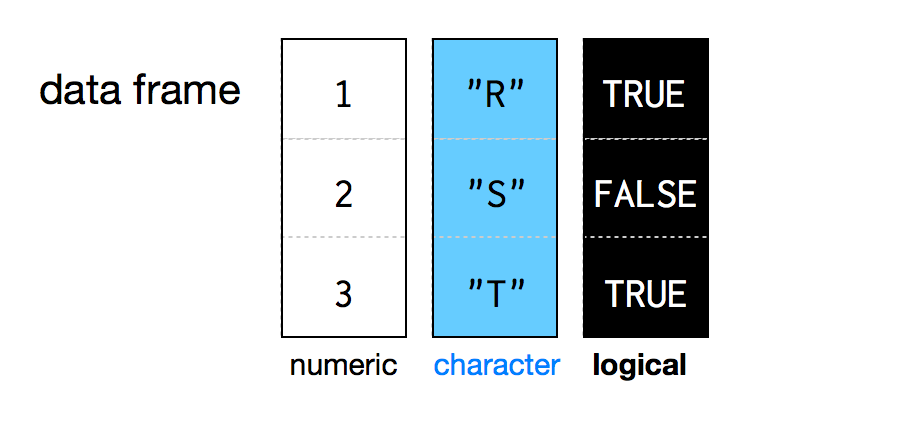
\includegraphics[width=650px]{images/data_frame_types} \caption{Data frames}\label{fig:unnamed-chunk-103}
\end{figure}

Data frames store data as a sequence of columns. Each column can be a different data type. Every column in a data frame must be the same length.

Creating a data frame by hand takes a lot of typing, but you can do it (if you like) with the \texttt{data.frame} function. Give \texttt{data.frame} any number of vectors, each separated with a comma. Each vector should be set equal to a name that describes the vector. \texttt{data.frame} will turn each vector into a column of the new data frame:

\begin{Shaded}
\begin{Highlighting}[]
\NormalTok{df }\OtherTok{\textless{}{-}} \FunctionTok{data.frame}\NormalTok{(}\AttributeTok{Subject\_id =} \FunctionTok{c}\NormalTok{(}\DecValTok{1}\NormalTok{,}\DecValTok{2}\NormalTok{,}\DecValTok{3}\NormalTok{, }\DecValTok{4}\NormalTok{),}
                 \AttributeTok{Gender =} \FunctionTok{c}\NormalTok{(}\StringTok{"female"}\NormalTok{, }\StringTok{"female"}\NormalTok{, }\StringTok{"male"}\NormalTok{, }\StringTok{"male"}\NormalTok{ ),}
                 \AttributeTok{IQ=}\FunctionTok{c}\NormalTok{(}\DecValTok{102}\NormalTok{, }\DecValTok{121}\NormalTok{, }\DecValTok{112}\NormalTok{, }\DecValTok{103}\NormalTok{),}
                 \AttributeTok{International\_student =} \FunctionTok{c}\NormalTok{(}\ConstantTok{FALSE}\NormalTok{, }\ConstantTok{FALSE}\NormalTok{, }\ConstantTok{TRUE}\NormalTok{, }\ConstantTok{FALSE}\NormalTok{))}
\end{Highlighting}
\end{Shaded}

You'll need to make sure that each vector is the same length. The resulting data frame looks like this:

\begin{Shaded}
\begin{Highlighting}[]
\FunctionTok{print}\NormalTok{(df)}
\end{Highlighting}
\end{Shaded}

\begin{verbatim}
##   Subject_id Gender  IQ International_student
## 1          1 female 102                 FALSE
## 2          2 female 121                 FALSE
## 3          3   male 112                  TRUE
## 4          4   male 103                 FALSE
\end{verbatim}

\begin{important}
Remember: \textbf{Use the \texttt{=} assignment inside functions}

Since you \texttt{data.frame} is a function and \texttt{Subject\_id},
\texttt{Gender}, \texttt{IQ} and \texttt{International\_student} are
arguments of this function, you have to use the equal sign \texttt{=} to
map the vectors to variable names and not the left hand side assignment
\texttt{\textless{}-}.
\end{important}

\subsubsection*{Variable overview}\label{variable-overview}
\addcontentsline{toc}{subsubsection}{Variable overview}

To function \texttt{str()} gives you a side-wise overview of the variables in a data frame. This show the variable names, the data types and the first few data points:

\begin{Shaded}
\begin{Highlighting}[]
\FunctionTok{str}\NormalTok{(df)}
\end{Highlighting}
\end{Shaded}

\begin{verbatim}
## 'data.frame':    4 obs. of  4 variables:
##  $ Subject_id           : num  1 2 3 4
##  $ Gender               : chr  "female" "female" "male" "male"
##  $ IQ                   : num  102 121 112 103
##  $ International_student: logi  FALSE FALSE TRUE FALSE
\end{verbatim}

\subsubsection*{Descriptive summary}\label{descriptive-summary}
\addcontentsline{toc}{subsubsection}{Descriptive summary}

A descriptive summary of all variables a data frame is very handy and important to check your data quality and to exclude potential technical issue in your dataset. It's very simply to do by:

\begin{Shaded}
\begin{Highlighting}[]
\FunctionTok{summary}\NormalTok{(df)}
\end{Highlighting}
\end{Shaded}

\begin{verbatim}
##    Subject_id      Gender                IQ        International_student
##  Min.   :1.00   Length:4           Min.   :102.0   Mode :logical        
##  1st Qu.:1.75   Class :character   1st Qu.:102.8   FALSE:3              
##  Median :2.50   Mode  :character   Median :107.5   TRUE :1              
##  Mean   :2.50                      Mean   :109.5                        
##  3rd Qu.:3.25                      3rd Qu.:114.2                        
##  Max.   :4.00                      Max.   :121.0
\end{verbatim}

\textbf{You should always do quality checks like this, if you read in tabular data.}

\begin{myexercise}
\textbf{Quality check}

Below you see summarizing information about dataset call
\texttt{demo\_data}. Without knowing the data in detail, what is strange
in this dataset?
\end{myexercise}

\begin{Shaded}
\begin{Highlighting}[]
\FunctionTok{nrow}\NormalTok{(demo\_data)}
\end{Highlighting}
\end{Shaded}

\begin{verbatim}
## [1] 200
\end{verbatim}

\begin{Shaded}
\begin{Highlighting}[]
\FunctionTok{summary}\NormalTok{(demo\_data)}
\end{Highlighting}
\end{Shaded}

\begin{verbatim}
##    variable_a        variable_b         variable_c
##  Min.   :-238.72   Min.   :-3.11356   Min.   :10  
##  1st Qu.:  14.18   1st Qu.:-0.71431   1st Qu.:10  
##  Median :  79.38   Median : 0.03375   Median :10  
##  Mean   :  79.42   Mean   : 0.01470   Mean   :10  
##  3rd Qu.: 144.05   3rd Qu.: 0.77758   3rd Qu.:10  
##  Max.   : 372.43   Max.   : 2.39493   Max.   :10  
##                    NA's   :131
\end{verbatim}

\webexhide{Solution}

The summary of this dataset shows that

\begin{enumerate}
\def\labelenumi{\arabic{enumi}.}
\tightlist
\item
  you have many missing values in \texttt{variable\_b} (131 out of 200 rows).
\item
  \texttt{variable\_b} comprises always of the same value 10 and has thus no variance. This might be a problem for you later statistical analyses.
\end{enumerate}

\webexunhide

\subsection{Subsetting}\label{nolabel}

\subsubsection{Selecting columns by name}\label{selectbyname}

You can access a specific column/variable of the data frame with \texttt{\$} \hyperref[listsdollar]{operator} as you know it from \hyperref[lists]{lists}. For example:

\begin{Shaded}
\begin{Highlighting}[]
\NormalTok{df}\SpecialCharTok{$}\NormalTok{IQ}
\end{Highlighting}
\end{Shaded}

\begin{verbatim}
## [1] 102 121 112 103
\end{verbatim}

As you see above, if you access a variable of a data frame with the \texttt{\$} operator, you get an \hyperref[vectors]{atomic vector}. This means that you can use subsetting of vectors as described in section \ref{subsetting}.

\begin{Shaded}
\begin{Highlighting}[]
\NormalTok{g }\OtherTok{\textless{}{-}}\NormalTok{ df}\SpecialCharTok{$}\NormalTok{Gender   }\CommentTok{\# g is a vector with the genders}
\NormalTok{g[}\DecValTok{2}\NormalTok{]             }\CommentTok{\# print the gender at the second positions}
\end{Highlighting}
\end{Shaded}

\begin{verbatim}
## [1] "female"
\end{verbatim}

But this can be done also in one expression.

\begin{Shaded}
\begin{Highlighting}[]
\NormalTok{df}\SpecialCharTok{$}\NormalTok{Gender[}\DecValTok{2}\NormalTok{]   }\CommentTok{\# get the Gender in the second row position}
\end{Highlighting}
\end{Shaded}

\begin{verbatim}
## [1] "female"
\end{verbatim}

\begin{myexercise}
\begin{itemize}
\tightlist
\item
  Calculate the median of the IQs of the subjects in the data frame.
\item
  Make a vector of logicals that is \texttt{TRUE} for all students that
  have an IQ larger than the mean IQ (and \texttt{FALSE} otherwise).
  Include this vector as new variable \texttt{is\_clever} to our data
  frame.
\end{itemize}
\end{myexercise}
\webexhide{Solution}

\begin{Shaded}
\begin{Highlighting}[]
\NormalTok{m\_iq }\OtherTok{=} \FunctionTok{mean}\NormalTok{(df}\SpecialCharTok{$}\NormalTok{IQ)}
\NormalTok{m\_iq}
\end{Highlighting}
\end{Shaded}

\begin{verbatim}
## [1] 109.5
\end{verbatim}

\begin{Shaded}
\begin{Highlighting}[]
\NormalTok{df}\SpecialCharTok{$}\NormalTok{is\_clever }\OtherTok{\textless{}{-}}\NormalTok{ df}\SpecialCharTok{$}\NormalTok{IQ }\SpecialCharTok{\textgreater{}}\NormalTok{ m\_iq}
\NormalTok{df}
\end{Highlighting}
\end{Shaded}

\begin{verbatim}
##   Subject_id Gender  IQ International_student is_clever
## 1          1 female 102                 FALSE     FALSE
## 2          2 female 121                 FALSE      TRUE
## 3          3   male 112                  TRUE      TRUE
## 4          4   male 103                 FALSE     FALSE
\end{verbatim}

\webexunhide

\subsubsection{Selecting by row and column indices}\label{selecting-by-row-and-column-indices}

Cells in an data frame can be also access via row and column indices and the \texttt{{[}{]}} operator. The syntax looks like this: \texttt{{[}row\_index,\ column\_index{]}}.

\begin{Shaded}
\begin{Highlighting}[]
\CommentTok{\# Check what you get}
\NormalTok{df[}\DecValTok{1}\NormalTok{, }\DecValTok{3}\NormalTok{]             }\CommentTok{\# returns from the 1st row the column 3}
\NormalTok{df[}\DecValTok{2}\SpecialCharTok{:}\DecValTok{4}\NormalTok{, }\DecValTok{3}\NormalTok{]           }\CommentTok{\# returns from row 2{-}4 the column 2}
\NormalTok{df[}\FunctionTok{c}\NormalTok{(}\DecValTok{1}\NormalTok{, }\DecValTok{4}\NormalTok{), }\FunctionTok{c}\NormalTok{(}\DecValTok{2}\NormalTok{,}\DecValTok{3}\NormalTok{)]  }\CommentTok{\# returns from row 1 and 4 the column 2 and 3}
\end{Highlighting}
\end{Shaded}

If you omit one of the indices \emph{R} takes all rows or columns of the omitted index.

\begin{Shaded}
\begin{Highlighting}[]
\NormalTok{df[, }\DecValTok{2}\NormalTok{]    }\CommentTok{\# all rows of column 2}
\NormalTok{df[}\DecValTok{4}\NormalTok{, ]    }\CommentTok{\# all columns of row 2 and 4}
\end{Highlighting}
\end{Shaded}

Consequently, \texttt{df{[},{]}} or \texttt{df{[}{]}} should return the entire data frame\ldots and this exactly what \emph{R} is doing.

\begin{myexercise}
\begin{itemize}
\tightlist
\item
  Access all columns from the 1st and 3rd row of \texttt{df}.
\item
  Do this also in an reversed order of the columns. That is, the first
  column should be \texttt{International\_student}.
\end{itemize}
\end{myexercise}
\webexhide{Solution}

\begin{Shaded}
\begin{Highlighting}[]
\NormalTok{df[}\FunctionTok{c}\NormalTok{(}\DecValTok{1}\NormalTok{, }\DecValTok{3}\NormalTok{), ]}
\end{Highlighting}
\end{Shaded}

\begin{verbatim}
##   Subject_id Gender  IQ International_student is_clever
## 1          1 female 102                 FALSE     FALSE
## 3          3   male 112                  TRUE      TRUE
\end{verbatim}

\begin{Shaded}
\begin{Highlighting}[]
\NormalTok{df[}\FunctionTok{c}\NormalTok{(}\DecValTok{1}\NormalTok{, }\DecValTok{3}\NormalTok{), }\DecValTok{4}\SpecialCharTok{:}\DecValTok{1}\NormalTok{]}
\end{Highlighting}
\end{Shaded}

\begin{verbatim}
##   International_student  IQ Gender Subject_id
## 1                 FALSE 102 female          1
## 3                  TRUE 112   male          3
\end{verbatim}

\webexunhide

\subsubsection{Subsetting with logicals}\label{subsettinglogicalsdataframe}

Section \ref{subsettinglogicals} demonstrated that you can select subsets with logicals. This subsetting with logical vectors is very useful for data frames and very often used. For example, if you want to have the data of the females only:

\begin{Shaded}
\begin{Highlighting}[]
\NormalTok{selected\_rows }\OtherTok{\textless{}{-}}\NormalTok{ df}\SpecialCharTok{$}\NormalTok{Gender }\SpecialCharTok{==} \StringTok{"female"}   \CommentTok{\# logical vector with TRUE for females}
\NormalTok{df[selected\_rows, ]}
\end{Highlighting}
\end{Shaded}

\begin{verbatim}
##   Subject_id Gender  IQ International_student is_clever
## 1          1 female 102                 FALSE     FALSE
## 2          2 female 121                 FALSE      TRUE
\end{verbatim}

Alternatively you can write it in one line:

\begin{Shaded}
\begin{Highlighting}[]
\NormalTok{df[df}\SpecialCharTok{$}\NormalTok{Gender }\SpecialCharTok{==} \StringTok{"female"}\NormalTok{, ]}
\end{Highlighting}
\end{Shaded}

\begin{myexercise}
Make a data frame with the clever people only.
\end{myexercise}
\webexhide{Solution}

\begin{Shaded}
\begin{Highlighting}[]
\NormalTok{clever }\OtherTok{\textless{}{-}}\NormalTok{ df[df}\SpecialCharTok{$}\NormalTok{is\_clever, ]  }\CommentTok{\# this clever is already a logical vector}
\NormalTok{clever}
\end{Highlighting}
\end{Shaded}

\begin{verbatim}
##   Subject_id Gender  IQ International_student is_clever
## 2          2 female 121                 FALSE      TRUE
## 3          3   male 112                  TRUE      TRUE
\end{verbatim}

\webexunhide

\subsection{Lists and data frames}\label{lists-and-data-frames}

Since lists and data frame can store multiple atomic vectors and they can actually both store tabular-like data. You can therefore convert between this two types using an \texttt{as.}-converter function. For instance, the list \texttt{lst} that we made in section \ref{listsdollar} can be converter to a data frame.

\begin{Shaded}
\begin{Highlighting}[]
\NormalTok{lst }\OtherTok{\textless{}{-}} \FunctionTok{list}\NormalTok{(}\AttributeTok{subjects=}\FunctionTok{c}\NormalTok{(}\StringTok{"John"}\NormalTok{, }\StringTok{"Maria"}\NormalTok{, }\StringTok{"Linda"}\NormalTok{),}
            \AttributeTok{body\_len=}\FunctionTok{c}\NormalTok{(}\FloatTok{1.92}\NormalTok{, }\FloatTok{1.71}\NormalTok{, }\FloatTok{1.63}\NormalTok{))}

\NormalTok{df2 }\OtherTok{\textless{}{-}} \FunctionTok{as.data.frame}\NormalTok{(lst)}
\NormalTok{df2}
\end{Highlighting}
\end{Shaded}

\begin{verbatim}
##   subjects body_len
## 1     John     1.92
## 2    Maria     1.71
## 3    Linda     1.63
\end{verbatim}

Note, converting a list to a data frame makes only sense, if the data in the list are indeed tabular, that is, if all objects in the list are atomic vectors of the same length.

Finally, a data frame can be converted into a list using \texttt{as.list()}. See what you get, if you convert the above data frame \texttt{df}:

\begin{Shaded}
\begin{Highlighting}[]
\FunctionTok{as.list}\NormalTok{(df)}
\end{Highlighting}
\end{Shaded}

\begin{verbatim}
## $Subject_id
## [1] 1 2 3 4
## 
## $Gender
## [1] "female" "female" "male"   "male"  
## 
## $IQ
## [1] 102 121 112 103
## 
## $International_student
## [1] FALSE FALSE  TRUE FALSE
## 
## $is_clever
## [1] FALSE  TRUE  TRUE FALSE
\end{verbatim}

\subsection{\texorpdfstring{Summary: Data structures in \emph{R}}{Summary: Data structures in R}}\label{summary-data-structures-in-r}

You can store data in \emph{R} with five different objects, which let you store different types of values in different types of relationships. The most common data structures in the analysis of psychological data are \textbf{vectors}, \textbf{lists} and \textbf{data frames}. For the sake of completeness, you should know that \textbf{matrices} and \textbf{n-dimentinal arrays} also exists in \emph{R}---they are however not relevant for this course.

\begin{figure}
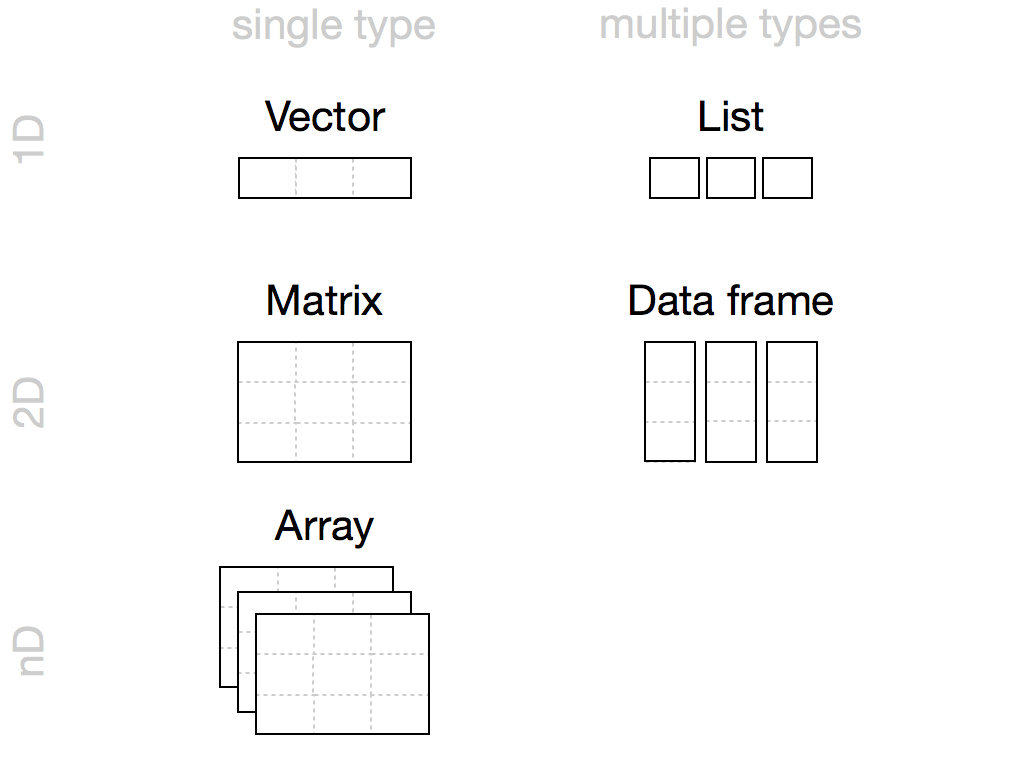
\includegraphics[width=650px]{images/r_data_types} \caption{Overview of data structures in R}\label{fig:unnamed-chunk-127}
\end{figure}

Importantly, data frames can store data of different types (e.g.~number, characters, text, factors, logical). Each column is conceptually a atomic vector and can thus only store data of one type. Data frames store the most common forms of data used in statistics, which are tabular data.

\section{Packages}\label{packages}

When you install \emph{R} you will have access to a range of functions including basic options for data wrangling and statistical analyses. The functions that are included in the default installation are typically referred to as \textbf{Base \emph{R}} and there is a useful \hyperref[cheatsheets]{cheat sheet} that shows many Base \emph{R} functions here. We've been using a couple functions from base \emph{R}, such as \texttt{seq()} or \texttt{rnorm()}-

However, the amazing power of \emph{R} is that it is extendable. That is, if a command or method doesn't exist anyone can create a so-called \emph{package} that contains one or multiple functions (and/or data) to perform new tasks. The large active \emph{R} user community is always creating new packages to expand \emph{R}'s capabilities. You may find it useful to think of Base \emph{R} as the default apps that come on your phone and packages as additional apps that you need to download separately.

In \emph{R} , the fundamental unit of shareable code is a package. A package bundles together code, data, documentation, and tests, and is easy to share with others. They increase the power of \emph{R} by improving existing base \emph{R} functionalities, or by adding new ones.

\subsection{Installing a package}\label{installing-a-package}

The traditional place to get \emph{R} packages is from \href{https://cran.r-project.org/}{\emph{CRAN}, the Comprehensive R Archive Network}, which is where you have downloaded \emph{R}.

However, you don't need to go to \emph{CRAN}'s website to install packages. It's much simpler and can be accomplished within the console using the command \texttt{install.packages("package-name-in-quotes")}. \emph{R} searches online on the \emph{CRAN} servers for a packages with that name and downloads and installs it locally. This works, of course, only if you have an internet connection. Let's install a small, fun package \texttt{praise}. You need to use quotes around the package name:

\begin{Shaded}
\begin{Highlighting}[]
\FunctionTok{install.packages}\NormalTok{(}\StringTok{"praise"}\NormalTok{)}
\end{Highlighting}
\end{Shaded}

\begin{myexercise}
The next chapters will make use of two packages that help us to
important data in \emph{R}. This packages are called \texttt{readr} and
\texttt{readxl}. Please install these two packages.
\end{myexercise}
\webexhide{Solution}

\begin{Shaded}
\begin{Highlighting}[]
\FunctionTok{install.packages}\NormalTok{(}\StringTok{"readr"}\NormalTok{)}
\FunctionTok{install.packages}\NormalTok{(}\StringTok{"readxl"}\NormalTok{)}
\end{Highlighting}
\end{Shaded}

\webexunhide

\begin{geek}
If you want to install multiple packages at once, you have to use a
vector of the package names you want to install as argument, e.g.,
\texttt{install.packages(\ c("package-a",\ "package-b")\ )}.
\end{geek}

\subsection{Using a package}\label{using-a-package}

So far, we've just installed packages. That is, the packages are now available on the local computer. Before we can use the new functionality, we need to tell \emph{R} to activate the package for this session, or better said, to load the library to memory. This will be done by the function \texttt{library()}. For example, to use the \texttt{praise}-package we call first:

\begin{Shaded}
\begin{Highlighting}[]
\FunctionTok{library}\NormalTok{(}\StringTok{"praise"}\NormalTok{)}
\end{Highlighting}
\end{Shaded}

Now that the \texttt{praise} package is loaded, you can use the function in that package. The new function is called \texttt{praise()} and returns a praise to make you feel better.

\begin{Shaded}
\begin{Highlighting}[]
\FunctionTok{praise}\NormalTok{()}
\end{Highlighting}
\end{Shaded}

\begin{verbatim}
## [1] "You are funkadelic!"
\end{verbatim}

\emph{(As you see, you can do really useful things with \emph{R} \texttt{;-)})}

\textbf{But what's the difference between a package and a library?}

Sometimes there is a confusion between a package and a library. Please don't get confused. You can find many people calling ``libraries'' to packages (like me, sometimes). To be precise, a library is a the collection of functions that we use in \emph{R} and that will be loaded into memory with the \texttt{library()}-command. A package is the bundle of software that you have to install to get the library. A package can contain more than just the library, for instance, documentation, example scripts and data.

\subsubsection*{\texorpdfstring{The \texttt{::} operator}{The :: operator}}\label{the-operator}
\addcontentsline{toc}{subsubsection}{The \texttt{::} operator}

Once you have load the package with \texttt{library()} \emph{R} knows all functions of that package and you can run the function just by calling it's name (as you know it).

If you call a function, it's also possible to mention explicitly the package from which the function stems. This is done with the \texttt{::} operator that separates the package and function name: \texttt{package-name::function-name()}. For example, calling the function \texttt{praise()} from the package \texttt{praise} would look like this:

\begin{Shaded}
\begin{Highlighting}[]
\NormalTok{praise}\SpecialCharTok{::}\FunctionTok{praise}\NormalTok{()}
\end{Highlighting}
\end{Shaded}

\textbf{Why should I use the \texttt{::} syntax?}

You don't have to use \texttt{::} and I guess that you will hardly need it for you own analyses. However, there are some reasons why you should know that this syntax exists:

\begin{enumerate}
\def\labelenumi{\arabic{enumi}.}
\tightlist
\item
  In manuals and documentations people often use this syntax to make clear from which package a particular function stems and which package needs to be installed to make use of this function.
\item
  If you use the \texttt{::} operator, you don't have to call \texttt{library()}. That is, if you need a function just once, it might be convenient to save a line of code.
\item
  It is possible that you use two packages that introduce the same name for different functions. This causes a naming conflict and one package masks the function of the other package. To get access to both functions in the different packages, you need to use the \texttt{::} operator.
\end{enumerate}

\begin{geek}
Mask conflicts occur for instance in the \texttt{tidyverse} package
collection, that we'll use next week. Mask conflicts will be depicted as
warnings while loading (importing) a library.
\end{geek}

\subsection{Getting help for packages}\label{getting-help-for-packages}

If you want to know more about a package, you can use \emph{R}'s built-in help function: \texttt{help(package="package-name")}.

\begin{myexercise}
Try to access the documentation of the function \texttt{read\_excel} of
the newly installed \texttt{readxl}-package.
\end{myexercise}

\section{Importing Data}\label{importing-data}

A crucial function of a statistical software is of course the ability to read data from files. There are many different types of files that you might work with when doing data analysis. These different file types are usually distinguished by the three letter extension following a period at the end of the file name. Here are some examples of functions (and packages!) that you can use to import data from different file types:

\begin{longtable}[]{@{}
  >{\raggedright\arraybackslash}p{(\columnwidth - 6\tabcolsep) * \real{0.1857}}
  >{\raggedright\arraybackslash}p{(\columnwidth - 6\tabcolsep) * \real{0.3429}}
  >{\raggedright\arraybackslash}p{(\columnwidth - 6\tabcolsep) * \real{0.3429}}
  >{\raggedright\arraybackslash}p{(\columnwidth - 6\tabcolsep) * \real{0.1286}}@{}}
\toprule\noalign{}
\begin{minipage}[b]{\linewidth}\raggedright
Extension
\end{minipage} & \begin{minipage}[b]{\linewidth}\raggedright
File Type
\end{minipage} & \begin{minipage}[b]{\linewidth}\raggedright
Reading
\end{minipage} & \begin{minipage}[b]{\linewidth}\raggedright
Writing
\end{minipage} \\
\midrule\noalign{}
\endhead
\bottomrule\noalign{}
\endlastfoot
.Rdata, .Rds & \emph{R}'s own data format & \texttt{load()} or \texttt{readRDS()} & \texttt{save()} or \texttt{saveRDS()} \\
.csv & Comma-separated values & \texttt{readr::read\_csv()} & \texttt{readr::write\_csv()} \\
.tsv, .txt & Tab-separated values & \texttt{readr::read\_tsv()} & \texttt{readr::write\_tsv()} \\
.xls, .xlsx & Excel workbook & \texttt{readxl::read\_excel()} & -- \\
.sav & SPSS data & \texttt{haven::read\_sav()} & \texttt{haven::write\_sav()} \\
.dta & Stata data & \texttt{haven::read\_dta()} & \texttt{haven::write\_dta()} \\
\end{longtable}

As you see, different packages that are dealing with data import. You have already installed the packages \texttt{readxl} and \texttt{readr} in the previous exercise.

\textbf{Example data}: You find some example data files in the \href{./data}{data folder}.

\subsection{Import via RStudio interface}\label{import-via-rstudio-interface}

\emph{R} offers several ways to import data from a file. One way is RStudio's import functions (see this week's instruction video).

\textbf{.Rdata:} \emph{R} 's own data files (.Rdata) can be very easily imported just by clicking on the file in the file browser.

\begin{myexercise}
You find a file \texttt{babynames.Rdata} among the example data. It
contains the frequencies of names given to babies in the US since 1880.

Load the dataset (via double click). How many rows does this file have?
\end{myexercise}

\webexhide{Solution}

Almost two million rows: \texttt{1924664}
\webexunhide

\paragraph*{Other file types}\label{other-file-types}
\addcontentsline{toc}{paragraph}{Other file types}

To import data from other (non-\emph{R}) file types, you can use the import panel of RStudio.

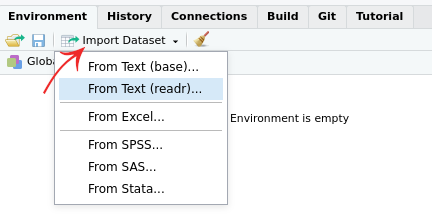
\includegraphics[width=350px]{images/data_import}

\subsection{Import via Console or Script}\label{import-via-console-or-script}

\subsubsection*{.Rdata}\label{rdata}
\addcontentsline{toc}{subsubsection}{.Rdata}

To load an \emph{R} data file via a script or the console, you called \texttt{load()} and the file path as argument. A file path consist of the subdirectory (relative to your current directory) and the filename separated by a \texttt{/} (backslash). For instance, if the data file is \texttt{babynames.Rdata} located in the subfolder \texttt{data}, this command should load the dataset:

\begin{Shaded}
\begin{Highlighting}[]
\FunctionTok{load}\NormalTok{(}\StringTok{"data/babynames.Rdata"}\NormalTok{)}
\end{Highlighting}
\end{Shaded}

\textbf{Hint:} You can use the autocompletion function of RStudio and type only \texttt{load("}, followed \texttt{TAB}.

\begin{important}
Since file paths are always relative to the \textbf{current working
directory}, you need to check in which directory you are currently in
(or in which folder the current script is).

The console displays the current working directory on top of the console
panel. Also the command \texttt{getcw()} gives you this information. The
autocompletion function is also handy here.
\end{important}

\subsubsection*{csv- and xlsx-files and other files}\label{csv--and-xlsx-files-and-other-files}
\addcontentsline{toc}{subsubsection}{csv- and xlsx-files and other files}

When you read in CSV files, it is best practice to use the \texttt{readr::read\_csv()} function. Note that you would normally want to store the result of the \texttt{read\_csv()} function to an object, as so:

\begin{Shaded}
\begin{Highlighting}[]
\FunctionTok{library}\NormalTok{(readr) }\CommentTok{\# load the package (just needed the first time)}
\NormalTok{csv\_data }\OtherTok{\textless{}{-}} \FunctionTok{read\_csv}\NormalTok{(}\StringTok{"data/exam\_anxiety.csv"}\NormalTok{)}
\end{Highlighting}
\end{Shaded}

The function \texttt{read\_excel()} from the package \texttt{readxl} is handy to read in Excel spreadsheet data.

A summary of data import function can be found in this \hyperref[cheatsheets]{data import cheat sheet}.

\newpage

\part{Data Wrangling}\label{part-data-wrangling}

\section{Tidyverse package collection}\label{tidyverse-package-collection}

\emph{Tidyverse} (\url{https://www.tidyverse.org/}) is a collection of \texttt{R} packages created by data scientist \href{http://hadley.nz/}{Hadley Wickham}, who has massively influenced the development \emph{R} in the recent decade. \emph{Tidyverse} contains several core packages (for example, \texttt{dplyr}, \texttt{tidyr}, \texttt{readr}, \texttt{purrr}, \texttt{ggplot2}, and \texttt{tibble}). It intends to facilitates the handling and visualization of data. After Wickham released these packages, they became heavily used in the \emph{R} community and are, in my view, the new quasi-standard of \emph{R} programming.

\begin{center}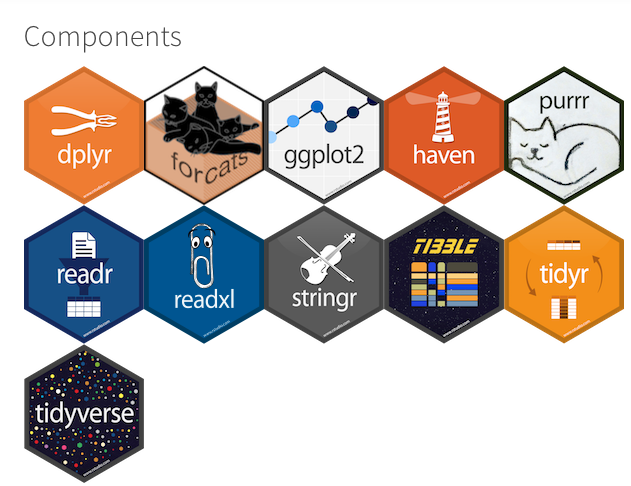
\includegraphics[width=300px]{images/tidyverse_components} \end{center}

In the core ten packages of \emph{Tidyverse} (see figure above), you find everything you need to preprocess and prepare you data for statistical analyses. We will therefore make use of \emph{Tidyverse} in the rest of this courses.

\begin{important}
Why not doing everything with base-\emph{R}?

Of course, all things that we do with \emph{Tidyverse} can be also
somehow done with the base \emph{R} commands, which we know already.
However, the commands of \emph{Tidyverse} are very powerful and, most
importantly, they result in a computer code that is much more readably
than the ugly base-\emph{R} code.

\textbf{The readability of the \emph{R}-scripts is very important,
because make it makes the data analyses less error-prone.}
\end{important}

\subsubsection*{Installing}\label{installing}
\addcontentsline{toc}{subsubsection}{Installing}

\emph{Tidyverse} is actually not really a package, but a meta-package, that is, a collection of packages. That is, if you install \emph{Tidyverse}, you install several packages. \textbf{It will therefore takes some time to install it}, especially on old machines.

\begin{Shaded}
\begin{Highlighting}[]
\FunctionTok{install.packages}\NormalTok{(}\StringTok{"tidyverse"}\NormalTok{)}
\end{Highlighting}
\end{Shaded}

\emph{Remark}: \textbf{MacOS} or \textbf{Linux} users that get an error when installing \emph{Tidyverse} need to install first some additional programs (see \hyperref[tidyverseinstall]{workaround} \ref{tidyverseinstall}).

\subsubsection*{Importing}\label{importing}
\addcontentsline{toc}{subsubsection}{Importing}

As with all \emph{R} -packages, if you want to make use of it in yours scripts, you need to import it first:

\begin{Shaded}
\begin{Highlighting}[]
\FunctionTok{library}\NormalTok{(tidyverse)}
\end{Highlighting}
\end{Shaded}

\begin{verbatim}
## -- Attaching core tidyverse packages ----------------------------------------------------------------------------------- tidyverse 2.0.0 --
## v dplyr     1.1.4     v readr     2.1.5
## v forcats   1.0.0     v stringr   1.5.1
## v ggplot2   3.5.1     v tibble    3.2.1
## v lubridate 1.9.3     v tidyr     1.3.1
## v purrr     1.0.2     
## -- Conflicts ----------------------------------------------------------------------------------------------------- tidyverse_conflicts() --
## x dplyr::filter() masks stats::filter()
## x dplyr::lag()    masks stats::lag()
## i Use the conflicted package (<http://conflicted.r-lib.org/>) to force all conflicts to become errors
\end{verbatim}

\begin{verbatim}
## ── Attaching packages ───────────────────────────────────────── tidyverse 1.3.0 ──
## ✓ ggplot2 3.3.2     ✓ purrr   0.3.4
## ✓ tibble  3.0.3     ✓ dplyr   1.0.0
## ✓ tidyr   1.1.0     ✓ stringr 1.4.0
## ✓ readr   1.3.1     ✓ forcats 0.5.0
## ── Conflicts ──────────────────────────────────────────── ## tidyverse_conflicts() ──
## x dplyr::filter() masks stats::filter()
## x dplyr::lag()    masks stats::lag()
\end{verbatim}

If you import the \emph{Tidyverse}-package with the \texttt{library()}-command you see that several core packages will be imported. The names of this packages are not really important here, you should just be aware that you can also import the single sub-packages separately. You see that often in code examples, if you check the help pages of \emph{R} or if you google for solutions in data processing.

\subsection{Tibble is the new Data Frame}\label{tibble-is-the-new-data-frame}

\emph{Tidyverse} introduces a new type of \texttt{data.frame}, called \texttt{tibble}. You use tibbles exactly like data frames and it does not really matter for you, whether you have a tibble or a data frame. \emph{R} converts a data frame automatically into a tibble whenever that is required and possible. I use the two labels therefore sometimes interchangeably.

You just need to know that a \texttt{tibble} is a modern version of a data frame, because it will show up in the \emph{R} output and in some scripts and documentations. Actually, we have already worked with the tibbles, because the data frames that you created when importing csv-files with the function \texttt{read\_csv} are tibbles and not base-\emph{R} data frames. Why? The package \texttt{readr} that we use for the import is part of the \emph{Tidyverse}.

The output of tibble is somewhat nicer that the output of data frames. But the difference is really minor. Check it out:

\begin{Shaded}
\begin{Highlighting}[]
\FunctionTok{library}\NormalTok{(readr) }\CommentTok{\# load the package (just needed the first time)}
\NormalTok{csv\_data }\OtherTok{\textless{}{-}} \FunctionTok{read\_csv}\NormalTok{(}\StringTok{"data/exam\_anxiety.csv"}\NormalTok{)}
\FunctionTok{print}\NormalTok{(csv\_data)}
\end{Highlighting}
\end{Shaded}

The first row shows that it is a tibble. The second row depicts the variable names and the third row shows the data type of the variable (\texttt{dbl} stands for ``double'' that is a numerical).

\begin{geek}
You can convert a data frame to a tibble with the function
\texttt{as\_tibble()} and a tibble into a data.frame with
\texttt{as.data.frame()}.
\end{geek}

\subsection{\texorpdfstring{Naming convention (``\texttt{\_}'' or ``\texttt{.}'')}{Naming convention (``\_'' or ``.'')}}\label{naming-convention-_-or-.}

If you are unsure whether a function is from \emph{Tidyverse} or part of base-\emph{R}, the function name often gives you a hint. \emph{Tidyverse} functions use always an underscore sign (\texttt{\_}) in the function names; for example \texttt{as\_tibble()}, the function to convert sometimes into a tibble. Classic base-\emph{R} uses the dot (\texttt{.}) in names, like in \texttt{as.numeric()} or \texttt{as.data.frame()}. This has historical reasons, because \emph{R} is inspired by the \href{https://en.wikipedia.org/wiki/S_(programming_language)}{programming language \emph{S}}, a language form the 70th. In that time the underscore was not a key on all computer keyboards.

I personally also prefer to use the underscore sign (as you have seen in the examples of this manual), because it's better readable and in line with naming conversions in other programming languages often used for data processing like \href{https://www.python.org/}{Python}, \href{https://julialang.org/}{Julia} or \href{https://en.wikipedia.org/wiki/MATLAB}{MATLAB}. Since more and more \emph{R}-users work with \emph{Tidyverse} the naming convention is currently also changing in the \emph{R}-community---that is at least my impression.

\section{Transforming Data}\label{transformingdata}

\subsubsection*{Example data}\label{example-data}
\addcontentsline{toc}{subsubsection}{Example data}

To illustrate the \emph{Tidyverse}-functions for data transformation, we use an example dataset \texttt{teaching\_method.csv} from that \href{./data}{data folder}.

The fake dataset looks like this (only 6 first rows are depicted):

\begin{table}

\caption{\label{tab:unnamed-chunk-148}First row of the example dataset 'teaching method'.}
\centering
\begin{tabular}[t]{rlllrr}
\toprule
student & teaching\_method & city & time & statistics & cog\_psy\\
\midrule
1 & method\_A & Groningen & before & 6 & 10\\
2 & method\_B & Nijmegen & before & 11 & 13\\
3 & control & Rotterdam & before & 12 & 10\\
4 & method\_A & Utrecht & before & 10 & 9\\
5 & method\_B & Nijmegen & before & 9 & 8\\
\addlinespace
6 & control & Utrecht & before & 8 & 11\\
\bottomrule
\end{tabular}
\end{table}

Students from universities in different Dutch cities were taught in statistics and cognitive psychology. Two teaching methods were compared (method A \& B). There was in addition a control condition with no teaching at all. The knowledge about the subjects was tested before and after the courses with a test of 40 questions and 4 choices. The results of the test (number of correct answers) for the two subjects are shown in the variables \texttt{statistcs} and \texttt{cog\_psy}.

Let's load \emph{Tidyverse} and the dataset:

\begin{Shaded}
\begin{Highlighting}[]
\FunctionTok{library}\NormalTok{(tidyverse)}
\NormalTok{teach }\OtherTok{\textless{}{-}} \FunctionTok{read\_csv}\NormalTok{(}\StringTok{"data/teaching\_method.csv"}\NormalTok{)}
\end{Highlighting}
\end{Shaded}

The import dataset is a tibble and looks in the console of RStudio like this:

\begin{Shaded}
\begin{Highlighting}[]
\FunctionTok{print}\NormalTok{(teach)}
\end{Highlighting}
\end{Shaded}

\begin{verbatim}
## # A tibble: 60 x 6
##    student teaching_method city      time   statistics cog_psy
##      <dbl> <chr>           <chr>     <chr>       <dbl>   <dbl>
##  1       1 method_A        Groningen before          6      10
##  2       2 method_B        Nijmegen  before         11      13
##  3       3 control         Rotterdam before         12      10
##  4       4 method_A        Utrecht   before         10       9
##  5       5 method_B        Nijmegen  before          9       8
##  6       6 control         Utrecht   before          8      11
##  7       7 method_A        Leiden    before          8      12
##  8       8 method_B        Utrecht   before          9      12
##  9       9 control         Leiden    before          8      10
## 10      10 method_A        Groningen before         10      12
## # i 50 more rows
\end{verbatim}

\subsection{\texorpdfstring{Selecting rows: \texttt{Filter()}}{Selecting rows: Filter()}}\label{selecting-rows-filter}

\begin{center}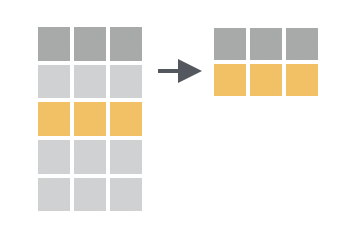
\includegraphics[width=300px]{images/dplyr-filter} \end{center}

We have already selected rows or cases of data frames with base-\emph{R} (see for last assignment or \hyperref[subsettinglogicalsdataframe]{section} \ref{subsettinglogicalsdataframe} ). If we want to select all students from Rotterdam, we would do it in base-\emph{R} like this:

\begin{Shaded}
\begin{Highlighting}[]
\NormalTok{teach[teach}\SpecialCharTok{$}\NormalTok{city }\SpecialCharTok{==} \StringTok{"Rotterdam"}\NormalTok{, ]}
\end{Highlighting}
\end{Shaded}

With \emph{Tidyverse} this can be done much more easily with function \texttt{filter()}.

\begin{Shaded}
\begin{Highlighting}[]
\FunctionTok{filter}\NormalTok{(teach, city }\SpecialCharTok{==} \StringTok{"Rotterdam"}\NormalTok{)}
\end{Highlighting}
\end{Shaded}

Of curse, you can use any logical comparisons that are possible in \emph{R}. For example, if you want to have all rows, which are not a control condition or all rows where \texttt{cog\_psy} is smaller 15:

\begin{Shaded}
\begin{Highlighting}[]
\FunctionTok{filter}\NormalTok{(teach, teaching\_method }\SpecialCharTok{!=} \StringTok{"control"}\NormalTok{)}
\FunctionTok{filter}\NormalTok{(teach, cog\_psy }\SpecialCharTok{\textless{}} \DecValTok{15}\NormalTok{)}
\end{Highlighting}
\end{Shaded}

This table gives an overview of of logical comparisons in \emph{R}:

\begin{center}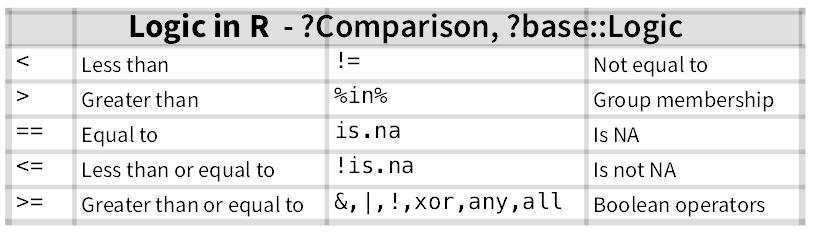
\includegraphics[width=500px]{images/logic_in_r} \end{center}

\subsubsection{Multiple criteria}\label{multiple-criteria}

\textbf{logical ``AND''}

The great thing with \emph{Tidyverse} is that you can very easy combine the filtering conditions. For instance, all cases in which the \texttt{city} is ``Rotterdam'' and the \texttt{time} is ``after'' and the \texttt{teaching\_method} is not ``control''.

\begin{Shaded}
\begin{Highlighting}[]
\FunctionTok{filter}\NormalTok{(teach, city}\SpecialCharTok{==}\StringTok{"Rotterdam"} \SpecialCharTok{\&}\NormalTok{ time}\SpecialCharTok{==}\StringTok{"after"} \SpecialCharTok{\&}\NormalTok{ teaching\_method}\SpecialCharTok{!=}\StringTok{"control"}\NormalTok{)}
\end{Highlighting}
\end{Shaded}

\begin{verbatim}
## # A tibble: 4 x 6
##   student teaching_method city      time  statistics cog_psy
##     <dbl> <chr>           <chr>     <chr>      <dbl>   <dbl>
## 1      13 method_A        Rotterdam after         26      40
## 2      17 method_B        Rotterdam after         30      33
## 3      19 method_A        Rotterdam after         34      32
## 4      29 method_B        Rotterdam after         22      23
\end{verbatim}

The sign \texttt{\&} is used in \emph{R} as logical \emph{and}.

\textbf{logical ``OR''}

The sign \texttt{\textbar{}} is used in \emph{R} as logical \emph{or}. For example, to select all rows, in which have test score in \texttt{statistics} lower 8 \textbf{or} in \texttt{cog\_psy} lower 6.

\begin{Shaded}
\begin{Highlighting}[]
\FunctionTok{filter}\NormalTok{(teach, statistics}\SpecialCharTok{\textless{}} \DecValTok{8} \SpecialCharTok{|}\NormalTok{ cog\_psy }\SpecialCharTok{\textless{}} \DecValTok{6}\NormalTok{)}
\end{Highlighting}
\end{Shaded}

\begin{verbatim}
## # A tibble: 6 x 6
##   student teaching_method city      time   statistics cog_psy
##     <dbl> <chr>           <chr>     <chr>       <dbl>   <dbl>
## 1       1 method_A        Groningen before          6      10
## 2      27 control         Rotterdam before          4      12
## 3      29 method_B        Rotterdam before         12       5
## 4      18 control         Leiden    after           6      16
## 5      21 control         Nijmegen  after           7      11
## 6      27 control         Rotterdam after           4      11
\end{verbatim}

More information about logical operators in \emph{R} can be found for instance \href{https://r4ds.had.co.nz/transform.html\#logical-operators}{here}

\subsection{\texorpdfstring{Sorting rows: \texttt{arrange()}}{Sorting rows: arrange()}}\label{sorting-rows-arrange}

\begin{center}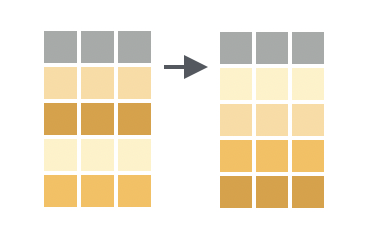
\includegraphics[width=300px]{images/dplyr-arrange} \end{center}

\texttt{arrange()} works similarly to \texttt{filter()} except that instead of selecting rows, it changes their order. It takes a data frame and a set of column names (or more complicated expressions) to order by.

\begin{Shaded}
\begin{Highlighting}[]
\NormalTok{teach }\OtherTok{\textless{}{-}} \FunctionTok{arrange}\NormalTok{(teach, statistics)   }\CommentTok{\# re{-}arrange \& override to old data frame}
\NormalTok{teach}
\end{Highlighting}
\end{Shaded}

\begin{verbatim}
## # A tibble: 60 x 6
##    student teaching_method city      time   statistics cog_psy
##      <dbl> <chr>           <chr>     <chr>       <dbl>   <dbl>
##  1      27 control         Rotterdam before          4      12
##  2      27 control         Rotterdam after           4      11
##  3       1 method_A        Groningen before          6      10
##  4      18 control         Leiden    after           6      16
##  5      21 control         Nijmegen  after           7      11
##  6       6 control         Utrecht   before          8      11
##  7       7 method_A        Leiden    before          8      12
##  8       9 control         Leiden    before          8      10
##  9      13 method_A        Rotterdam before          8      13
## 10      16 method_A        Nijmegen  before          8       9
## # i 50 more rows
\end{verbatim}

Use \texttt{desc()} to re-order by a column in descending order:

\begin{Shaded}
\begin{Highlighting}[]
\NormalTok{teach }\OtherTok{\textless{}{-}} \FunctionTok{arrange}\NormalTok{(teach, }\FunctionTok{desc}\NormalTok{(statistics))}
\NormalTok{teach}
\end{Highlighting}
\end{Shaded}

\begin{verbatim}
## # A tibble: 60 x 6
##    student teaching_method city      time  statistics cog_psy
##      <dbl> <chr>           <chr>     <chr>      <dbl>   <dbl>
##  1      28 method_A        Leiden    after         37      35
##  2      19 method_A        Rotterdam after         34      32
##  3       4 method_A        Utrecht   after         32      37
##  4      17 method_B        Rotterdam after         30      33
##  5      10 method_A        Groningen after         29      35
##  6       2 method_B        Nijmegen  after         28      40
##  7      11 method_B        Utrecht   after         28      31
##  8      16 method_A        Nijmegen  after         28      30
##  9      25 method_A        Groningen after         28      32
## 10       5 method_B        Nijmegen  after         27      29
## # i 50 more rows
\end{verbatim}

If you want to sort first by \texttt{city} and then by the \texttt{statistics} test score, you just provide more than one column name. Each additional listed column will be used to break ties in the values of preceding columns:

\begin{Shaded}
\begin{Highlighting}[]
\NormalTok{teach }\OtherTok{\textless{}{-}} \FunctionTok{arrange}\NormalTok{(teach, city, statistics) }\CommentTok{\# sort for city then for statistics}
\NormalTok{teach }\OtherTok{\textless{}{-}} \FunctionTok{arrange}\NormalTok{(teach, city, statistics) }\CommentTok{\# sort for statistics and then for city}
\end{Highlighting}
\end{Shaded}

\begin{myexercise}
Check out the different types of sorting and use RStudios object viewer
to see differently sorted data frames.
\end{myexercise}

\subsection{\texorpdfstring{Selecting \& Arranging Variables: \texttt{select()}}{Selecting \& Arranging Variables: select()}}\label{selecting-arranging-variables-select}

\subsubsection{Select a Variable}\label{select-a-variable}

\begin{center}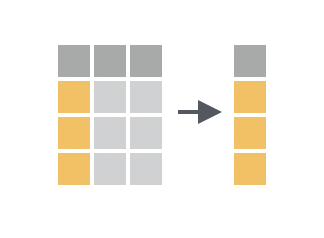
\includegraphics[width=300px]{images/dplyr-select} \end{center}

Selecting variables from a data frame was already easy in base-\emph{R} (see \hyperref[selectbyname]{section} \ref{selectbyname}{]}). \emph{Tidyverse} offers the function \texttt{select()} for this and you will see that it's even easier. \texttt{select()} more powerful when it come to selecting multiple variables and it improves the readability of your code.

It's not uncommon to get datasets with a large amount of variables. In this case, the first challenge is often narrowing in on the variables you're actually interested in. \texttt{select()} allows you to rapidly zoom in on a useful subset using operations based on the names of the variables.

Select the variable for our data frame \texttt{teach}:

\begin{Shaded}
\begin{Highlighting}[]
\FunctionTok{select}\NormalTok{(teach, cog\_psy)}
\end{Highlighting}
\end{Shaded}

\begin{verbatim}
## # A tibble: 60 x 1
##    cog_psy
##      <dbl>
##  1      35
##  2      32
##  3      37
##  4      33
##  5      35
##  6      40
##  7      31
##  8      30
##  9      32
## 10      29
## # i 50 more rows
\end{verbatim}

To select multiple variables just add further variables names as argument, separated by a comma:

\begin{Shaded}
\begin{Highlighting}[]
\FunctionTok{select}\NormalTok{(teach, cog\_psy, student, city)}
\end{Highlighting}
\end{Shaded}

\begin{verbatim}
## # A tibble: 60 x 3
##    cog_psy student city     
##      <dbl>   <dbl> <chr>    
##  1      35      28 Leiden   
##  2      32      19 Rotterdam
##  3      37       4 Utrecht  
##  4      33      17 Rotterdam
##  5      35      10 Groningen
##  6      40       2 Nijmegen 
##  7      31      11 Utrecht  
##  8      30      16 Nijmegen 
##  9      32      25 Groningen
## 10      29       5 Nijmegen 
## # i 50 more rows
\end{verbatim}

\subsubsection{Re-arranging the Order of Variables}\label{re-arranging-the-order-of-variables}

As you see the variables appear in the order you mentioned them in the command. Inn other words, you can use select also to re-arrange the order of your columns.

When re-arranging the order, another option is to use the \texttt{everything()} helper, which stands for all remaining variable. This is useful if you have a handful of variables you'd like to move to the start (or end) of the data frame.

\begin{Shaded}
\begin{Highlighting}[]
\FunctionTok{select}\NormalTok{(teach,  city, }\FunctionTok{everything}\NormalTok{())}
\end{Highlighting}
\end{Shaded}

\begin{verbatim}
## # A tibble: 60 x 6
##    city      student teaching_method time  statistics cog_psy
##    <chr>       <dbl> <chr>           <chr>      <dbl>   <dbl>
##  1 Leiden         28 method_A        after         37      35
##  2 Rotterdam      19 method_A        after         34      32
##  3 Utrecht         4 method_A        after         32      37
##  4 Rotterdam      17 method_B        after         30      33
##  5 Groningen      10 method_A        after         29      35
##  6 Nijmegen        2 method_B        after         28      40
##  7 Utrecht        11 method_B        after         28      31
##  8 Nijmegen       16 method_A        after         28      30
##  9 Groningen      25 method_A        after         28      32
## 10 Nijmegen        5 method_B        after         27      29
## # i 50 more rows
\end{verbatim}

\subsubsection{Dropping a Variable}\label{dropping-a-variable}

\begin{center}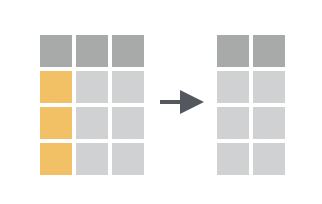
\includegraphics[width=300px]{images/dplyr-select-drop} \end{center}

If you want to exclude a column you just write \texttt{-} followed by the variable name:

\begin{Shaded}
\begin{Highlighting}[]
\FunctionTok{select}\NormalTok{(teach, }\SpecialCharTok{{-}}\NormalTok{city)}
\end{Highlighting}
\end{Shaded}

\begin{verbatim}
## # A tibble: 60 x 5
##    student teaching_method time  statistics cog_psy
##      <dbl> <chr>           <chr>      <dbl>   <dbl>
##  1      28 method_A        after         37      35
##  2      19 method_A        after         34      32
##  3       4 method_A        after         32      37
##  4      17 method_B        after         30      33
##  5      10 method_A        after         29      35
##  6       2 method_B        after         28      40
##  7      11 method_B        after         28      31
##  8      16 method_A        after         28      30
##  9      25 method_A        after         28      32
## 10       5 method_B        after         27      29
## # i 50 more rows
\end{verbatim}

\subsubsection{Select a Range of Variables}\label{select-a-range-of-variables}

\begin{center}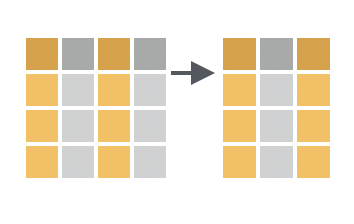
\includegraphics[width=300px]{images/dplyr-select-range} \end{center}

If you want to select all variable from column \texttt{city} to column \texttt{statistics}, it's very handy to use this \texttt{:}-operator. This operator only works for variable names for you use \emph{Tidyverse}.

\begin{Shaded}
\begin{Highlighting}[]
\FunctionTok{select}\NormalTok{(teach, city}\SpecialCharTok{:}\NormalTok{statistics)}
\end{Highlighting}
\end{Shaded}

\begin{verbatim}
## # A tibble: 60 x 3
##    city      time  statistics
##    <chr>     <chr>      <dbl>
##  1 Leiden    after         37
##  2 Rotterdam after         34
##  3 Utrecht   after         32
##  4 Rotterdam after         30
##  5 Groningen after         29
##  6 Nijmegen  after         28
##  7 Utrecht   after         28
##  8 Nijmegen  after         28
##  9 Groningen after         28
## 10 Nijmegen  after         27
## # i 50 more rows
\end{verbatim}

\subsection{\texorpdfstring{Add new variables: \texttt{mutate()}}{Add new variables: mutate()}}\label{add-new-variables-mutate}

\begin{center}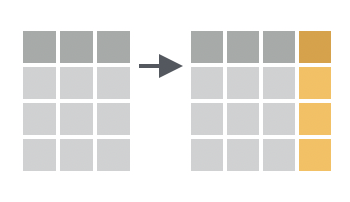
\includegraphics[width=300px]{images/dplyr-mutate} \end{center}

Very often you want to add new columns that are functions of existing columns. That's the job of \texttt{mutate()}.

\texttt{mutate()} always adds new columns at the end of your dataset. For instance, if you want to calculate the test scores (i.e., number of correct answers) into percentage, we have multiple the score with \(\frac{N_\text{questions}}{100}\)? We know the test had 40 questions, thus:

\begin{Shaded}
\begin{Highlighting}[]
\NormalTok{teach\_extended }\OtherTok{\textless{}{-}} \FunctionTok{mutate}\NormalTok{(teach, }\AttributeTok{percent\_statistics =}\NormalTok{ statistics }\SpecialCharTok{/} \DecValTok{40} \SpecialCharTok{*} \DecValTok{100}\NormalTok{)}
\NormalTok{teach\_extended}
\end{Highlighting}
\end{Shaded}

\begin{verbatim}
## # A tibble: 60 x 7
##    student teaching_method city      time  statistics cog_psy percent_statistics
##      <dbl> <chr>           <chr>     <chr>      <dbl>   <dbl>              <dbl>
##  1      28 method_A        Leiden    after         37      35               92.5
##  2      19 method_A        Rotterdam after         34      32               85  
##  3       4 method_A        Utrecht   after         32      37               80  
##  4      17 method_B        Rotterdam after         30      33               75  
##  5      10 method_A        Groningen after         29      35               72.5
##  6       2 method_B        Nijmegen  after         28      40               70  
##  7      11 method_B        Utrecht   after         28      31               70  
##  8      16 method_A        Nijmegen  after         28      30               70  
##  9      25 method_A        Groningen after         28      32               70  
## 10       5 method_B        Nijmegen  after         27      29               67.5
## # i 50 more rows
\end{verbatim}

You probably remember from last week, you can also do this with base \emph{R}:

\begin{Shaded}
\begin{Highlighting}[]
\NormalTok{teach}\SpecialCharTok{$}\NormalTok{percent\_statistics }\OtherTok{\textless{}{-}}\NormalTok{ teach}\SpecialCharTok{$}\NormalTok{statistics }\SpecialCharTok{/} \DecValTok{40} \SpecialCharTok{*} \DecValTok{100}
\end{Highlighting}
\end{Shaded}

However, \texttt{mutate()} becomes really convenient (and again produces simpler code), if you need to add several columns. Just like \texttt{arrange()} or \texttt{select()}, you can add further variables by adding another argument to the function call (separated with a comma):

\begin{Shaded}
\begin{Highlighting}[]
\NormalTok{teach\_extended }\OtherTok{\textless{}{-}} \FunctionTok{mutate}\NormalTok{(teach,}
                    \AttributeTok{percent\_statistics =}\NormalTok{ statistics }\SpecialCharTok{/} \DecValTok{40} \SpecialCharTok{*} \DecValTok{100}\NormalTok{,}
                    \AttributeTok{percent\_cog\_psy =}\NormalTok{ cog\_psy }\SpecialCharTok{/} \DecValTok{40} \SpecialCharTok{*} \DecValTok{100}\NormalTok{)}
\end{Highlighting}
\end{Shaded}

Check out how the resulting data frame \texttt{teach\_extended} looks like. Remember that when you're in RStudio, the easiest way to see all the columns is the object viewer using \texttt{View(teach\_extended)}.

\textbf{Hint for data frames with many variables}: To check a data frame with many variables in the console, the function \texttt{glimpse()} produces a nice vertical overview of all columns and the first data.

\webexhide{glimpse}

\begin{Shaded}
\begin{Highlighting}[]
\FunctionTok{glimpse}\NormalTok{(teach\_extended)}
\end{Highlighting}
\end{Shaded}

\begin{verbatim}
## Rows: 60
## Columns: 8
## $ student            <dbl> 28, 19, 4, 17, 10, 2, 11, 16, 25, 5, 1, 8, 13, 22, ~
## $ teaching_method    <chr> "method_A", "method_A", "method_A", "method_B", "me~
## $ city               <chr> "Leiden", "Rotterdam", "Utrecht", "Rotterdam", "Gro~
## $ time               <chr> "after", "after", "after", "after", "after", "after~
## $ statistics         <dbl> 37, 34, 32, 30, 29, 28, 28, 28, 28, 27, 26, 26, 26,~
## $ cog_psy            <dbl> 35, 32, 37, 33, 35, 40, 31, 30, 32, 29, 32, 36, 40,~
## $ percent_statistics <dbl> 92.5, 85.0, 80.0, 75.0, 72.5, 70.0, 70.0, 70.0, 70.~
## $ percent_cog_psy    <dbl> 87.5, 80.0, 92.5, 82.5, 87.5, 100.0, 77.5, 75.0, 80~
\end{verbatim}

\webexunhide

\begin{myexercise}
 Take the command above and calculate and add further variables. We want
 to have also for each row
 
 \begin{itemize}
 \tightlist
 \item
   the average score of both test (\texttt{mean\_score}) and
 \item
   the average percentage correct in both tests
   (\texttt{percent\_correct\_both}).
 \end{itemize}
 \end{myexercise}
\webexhide{Solution}

\begin{Shaded}
\begin{Highlighting}[]
\NormalTok{teach\_extended }\OtherTok{\textless{}{-}} \FunctionTok{mutate}\NormalTok{(teach, }\AttributeTok{percent\_statistics =}\NormalTok{ statistics}\SpecialCharTok{/}\DecValTok{40}\SpecialCharTok{*}\DecValTok{100}\NormalTok{,}
              \AttributeTok{percent\_cog\_psy =}\NormalTok{ cog\_psy}\SpecialCharTok{/}\DecValTok{40}\SpecialCharTok{*}\DecValTok{100}\NormalTok{,}
              \AttributeTok{mean\_score =}\NormalTok{ (statistics}\SpecialCharTok{+}\NormalTok{cog\_psy)}\SpecialCharTok{/}\DecValTok{2}\NormalTok{,}
              \AttributeTok{percent\_correct\_both =}\NormalTok{ mean\_score}\SpecialCharTok{/}\DecValTok{40}\SpecialCharTok{*}\DecValTok{100}\NormalTok{)}
\FunctionTok{glimpse}\NormalTok{(teach\_extended)}
\end{Highlighting}
\end{Shaded}

\begin{verbatim}
## Rows: 60
## Columns: 10
## $ student              <dbl> 28, 19, 4, 17, 10, 2, 11, 16, 25, 5, 1, 8, 13, 22~
## $ teaching_method      <chr> "method_A", "method_A", "method_A", "method_B", "~
## $ city                 <chr> "Leiden", "Rotterdam", "Utrecht", "Rotterdam", "G~
## $ time                 <chr> "after", "after", "after", "after", "after", "aft~
## $ statistics           <dbl> 37, 34, 32, 30, 29, 28, 28, 28, 28, 27, 26, 26, 2~
## $ cog_psy              <dbl> 35, 32, 37, 33, 35, 40, 31, 30, 32, 29, 32, 36, 4~
## $ percent_statistics   <dbl> 92.5, 85.0, 80.0, 75.0, 72.5, 70.0, 70.0, 70.0, 7~
## $ percent_cog_psy      <dbl> 87.5, 80.0, 92.5, 82.5, 87.5, 100.0, 77.5, 75.0, ~
## $ mean_score           <dbl> 36.0, 33.0, 34.5, 31.5, 32.0, 34.0, 29.5, 29.0, 3~
## $ percent_correct_both <dbl> 90.00, 82.50, 86.25, 78.75, 80.00, 85.00, 73.75, ~
\end{verbatim}

\webexunhide

\section{Summarizing \& Aggregating Data}\label{summarising}

\subsection{\texorpdfstring{Aggregating data with \texttt{summarise()}}{Aggregating data with summarise()}}\label{aggregating-data-with-summarise}

Create summary statistics for the dataset can be done with the command \texttt{summarise()}. Check the data transformation \hyperref[cheatsheets]{cheat sheet} for various summary functions. Some common ones are: \texttt{mean()}, \texttt{sd()}, \texttt{n()}, \texttt{sum()} or \texttt{quantile()}.

For instance,

\begin{Shaded}
\begin{Highlighting}[]
\NormalTok{summary\_df }\OtherTok{\textless{}{-}} \FunctionTok{summarise}\NormalTok{(teach,}
                \AttributeTok{n\_obs=}\FunctionTok{n}\NormalTok{(),}
                \AttributeTok{m\_statistics =} \FunctionTok{mean}\NormalTok{(statistics),}
                \AttributeTok{m\_cog\_psy =} \FunctionTok{mean}\NormalTok{(cog\_psy),}
                \AttributeTok{useless =} \FunctionTok{sum}\NormalTok{(statistics}\SpecialCharTok{+}\NormalTok{cog\_psy) )}
\FunctionTok{print}\NormalTok{(summary\_df)}
\end{Highlighting}
\end{Shaded}

\begin{verbatim}
## # A tibble: 1 x 4
##   n_obs m_statistics m_cog_psy useless
##   <int>        <dbl>     <dbl>   <dbl>
## 1    60         15.4      18.2    2017
\end{verbatim}

As you see this command generates a data frame (that we save in \texttt{summary\_df}) with the number of observations (\texttt{n\_obs}), the mean grade for statistics and cognitive psychology (\texttt{m\_statistics} \& \texttt{m\_cog\_psy}) and a \texttt{useless} variable that is sum off all scores in statistics and cognitive psychology. The mean grade in \texttt{statistics} is lower than in \texttt{cog\_psy}.

Ok, fine, but you may think now: ``I could get the same information much simpler with the base-\emph{R}. Why shall I use this strange \texttt{summarise()} thing?'' The actual power of it becomes clear if used together with the \texttt{group\_by()} command described in the next section.

\subsection{\texorpdfstring{Grouping data by \texttt{group\_by()}}{Grouping data by group\_by()}}\label{grouping-data-by-group_by}

If you want that all \emph{Tidyverse}-operations will be done separately for different parts of a tibble or data frame, you can group your data and use a grouped tibble. You group a data with the \texttt{group\_by()} command:

\begin{Shaded}
\begin{Highlighting}[]
\NormalTok{teach\_grouped }\OtherTok{\textless{}{-}} \FunctionTok{group\_by}\NormalTok{(teach, city)}
\FunctionTok{print}\NormalTok{(teach\_grouped)}
\end{Highlighting}
\end{Shaded}

\begin{verbatim}
## # A tibble: 60 x 6
## # Groups:   city [5]
##    student teaching_method city      time  statistics cog_psy
##      <dbl> <chr>           <chr>     <chr>      <dbl>   <dbl>
##  1      28 method_A        Leiden    after         37      35
##  2      19 method_A        Rotterdam after         34      32
##  3       4 method_A        Utrecht   after         32      37
##  4      17 method_B        Rotterdam after         30      33
##  5      10 method_A        Groningen after         29      35
##  6       2 method_B        Nijmegen  after         28      40
##  7      11 method_B        Utrecht   after         28      31
##  8      16 method_A        Nijmegen  after         28      30
##  9      25 method_A        Groningen after         28      32
## 10       5 method_B        Nijmegen  after         27      29
## # i 50 more rows
\end{verbatim}

You actually see nothing special happening and the new data frame \texttt{teach\_grouped} looks exactly like the \texttt{teach}. The curial difference is for \emph{R} that the new data frame is grouped. You see that in the second line of the output. The variable \texttt{city} defines the group. There are in total 5 groups.

If we now apply the \texttt{summarise()} command on the new group data, we get the aggregated data for separately for each group :

\begin{Shaded}
\begin{Highlighting}[]
\NormalTok{summary\_df }\OtherTok{\textless{}{-}} \FunctionTok{summarise}\NormalTok{(teach\_grouped,   }\CommentTok{\# use the new grouped df}
                \AttributeTok{n\_obs=}\FunctionTok{n}\NormalTok{(),}
                \AttributeTok{m\_statistics =} \FunctionTok{mean}\NormalTok{(statistics),}
                \AttributeTok{m\_cog\_psy =} \FunctionTok{mean}\NormalTok{(cog\_psy),}
                \AttributeTok{useless =} \FunctionTok{sum}\NormalTok{(statistics}\SpecialCharTok{+}\NormalTok{cog\_psy) )}
\FunctionTok{print}\NormalTok{(summary\_df)}
\end{Highlighting}
\end{Shaded}

\begin{verbatim}
## # A tibble: 5 x 5
##   city      n_obs m_statistics m_cog_psy useless
##   <chr>     <int>        <dbl>     <dbl>   <dbl>
## 1 Groningen    12         15.9      20.2     433
## 2 Leiden       12         12.8      15.7     341
## 3 Nijmegen     12         14.8      17.9     393
## 4 Rotterdam    12         15.7      17.4     397
## 5 Utrecht      12         17.9      19.8     453
\end{verbatim}

You see the aggregated data for each city. In each city we have 12 measures. In our fake dataset, the statistics grades seems to be on average higher in Utrecht than in Leiden.

\subsubsection*{Grouping for multiple variables}\label{grouping-for-multiple-variables}
\addcontentsline{toc}{subsubsection}{Grouping for multiple variables}

Like with the other \emph{Tidyverse} functions you can add variables and further group the dataset. Let's get the aggregated data for each \texttt{teaching\_method} and in each \texttt{city}:

\begin{Shaded}
\begin{Highlighting}[]
\NormalTok{teach\_grouped }\OtherTok{\textless{}{-}} \FunctionTok{group\_by}\NormalTok{(teach, city, teaching\_method)}
\NormalTok{summary\_df }\OtherTok{\textless{}{-}} \FunctionTok{summarise}\NormalTok{(teach\_grouped,}
                \AttributeTok{n\_obs=}\FunctionTok{n}\NormalTok{(),}
                \AttributeTok{m\_statistics =} \FunctionTok{mean}\NormalTok{(statistics),}
                \AttributeTok{m\_cog\_psy =} \FunctionTok{mean}\NormalTok{(cog\_psy),}
                \AttributeTok{useless =} \FunctionTok{sum}\NormalTok{(statistics}\SpecialCharTok{+}\NormalTok{cog\_psy) )}
\NormalTok{summary\_df}
\end{Highlighting}
\end{Shaded}

\begin{verbatim}
## # A tibble: 14 x 6
## # Groups:   city [5]
##    city      teaching_method n_obs m_statistics m_cog_psy useless
##    <chr>     <chr>           <int>        <dbl>     <dbl>   <dbl>
##  1 Groningen control             2        12         11        46
##  2 Groningen method_A            6        17.8       21.7     237
##  3 Groningen method_B            4        15         22.5     150
##  4 Leiden    control             8         9.88      11.9     174
##  5 Leiden    method_A            4        18.5       23.2     167
##  6 Nijmegen  control             4        10.2       11.8      88
##  7 Nijmegen  method_A            2        18         19.5      75
##  8 Nijmegen  method_B            6        16.8       21.5     230
##  9 Rotterdam control             4         8         11        76
## 10 Rotterdam method_A            4        20         23.5     174
## 11 Rotterdam method_B            4        19         17.8     147
## 12 Utrecht   control             2        11.5       12        47
## 13 Utrecht   method_A            4        19.5       22       166
## 14 Utrecht   method_B            6        19         21       240
\end{verbatim}

You see that the conditions are not evenly distributed over the cities. In Leiden were more students (8) in the control condition with no teaching than in Utrecht (2). This explains possibly the difference in the statistic grades.

\begin{myexercise}
Calculate the mean statistics grade separate for all
\texttt{teaching\_methods} and for the \texttt{time} before and after
the course.
\end{myexercise}
\webexhide{Solution}

\begin{Shaded}
\begin{Highlighting}[]
\FunctionTok{summarize}\NormalTok{(}\FunctionTok{group\_by}\NormalTok{(teach, time, teaching\_method), }\AttributeTok{m\_statistics =} \FunctionTok{mean}\NormalTok{(statistics))}
\end{Highlighting}
\end{Shaded}

\begin{verbatim}
## # A tibble: 6 x 3
## # Groups:   time [2]
##   time   teaching_method m_statistics
##   <chr>  <chr>                  <dbl>
## 1 after  control                 10.2
## 2 after  method_A                28.5
## 3 after  method_B                24.1
## 4 before control                  9.7
## 5 before method_A                 9  
## 6 before method_B                11
\end{verbatim}

\webexunhide

\begin{myexercise}
Are those who are better in statistics also better in cognitive
psychology?

Use a simple median-split comparison: Calculate the \texttt{median()} of
all statistics grades and calculate the mean cognitive psychology grade
for those who have higher grades than the median in statistics and those
who have lower grades.
\end{myexercise}
\webexhide{Solution}

\begin{Shaded}
\begin{Highlighting}[]
\NormalTok{teach2 }\OtherTok{\textless{}{-}} \FunctionTok{mutate}\NormalTok{(teach, }\AttributeTok{good\_in\_stats =}\NormalTok{ statistics}\SpecialCharTok{\textgreater{}}\FunctionTok{median}\NormalTok{(statistics))}
\NormalTok{teach2\_grouped }\OtherTok{\textless{}{-}} \FunctionTok{group\_by}\NormalTok{(teach2, good\_in\_stats)}
\FunctionTok{summarize}\NormalTok{(teach2\_grouped, }\AttributeTok{m\_cog\_psy =} \FunctionTok{mean}\NormalTok{(cog\_psy))}
\end{Highlighting}
\end{Shaded}

\begin{verbatim}
## # A tibble: 2 x 2
##   good_in_stats m_cog_psy
##   <lgl>             <dbl>
## 1 FALSE              10.7
## 2 TRUE               28.7
\end{verbatim}

..and for the geeks in one line of code:

\begin{Shaded}
\begin{Highlighting}[]
\FunctionTok{summarize}\NormalTok{(}\FunctionTok{group\_by}\NormalTok{(teach, statistics }\SpecialCharTok{\textgreater{}} \FunctionTok{median}\NormalTok{(statistics)), }
                                \AttributeTok{m\_cog\_psy =} \FunctionTok{mean}\NormalTok{(cog\_psy))}
\end{Highlighting}
\end{Shaded}

\begin{verbatim}
## # A tibble: 2 x 2
##   `statistics > median(statistics)` m_cog_psy
##   <lgl>                                 <dbl>
## 1 FALSE                                  10.7
## 2 TRUE                                   28.7
\end{verbatim}

TRUE is the group with a grade \texttt{\textgreater{}\ median(statistics)}. FALSE is the low stats group.
\webexunhide

\subsubsection*{Ungrouping a grouped data frame}\label{ungrouping-a-grouped-data-frame}
\addcontentsline{toc}{subsubsection}{Ungrouping a grouped data frame}

You can remove the grouping of a data frame with \texttt{ungroup()}.

\subsection{Summary}\label{summary}

The last two chapters introduced the following six \emph{Tidyverse} -commands, which all stems actually from the subpackage \texttt{dplyr} in the \texttt{tidyverse}.

\begin{itemize}
\item
  \texttt{filter()} Include or exclude certain cases (rows)
\item
  \texttt{arrange()} Change the order of cases (rows)
\item
  \texttt{select()} Include or exclude certain variables (columns)
\item
  \texttt{mutate()} Create new variables (columns)
\item
  \texttt{summarise()} Derive aggregate variables for groups of observations
  subsequent
\item
  \texttt{group\_by()} Organize the data into groups
\end{itemize}

These six functions are known as 'single table verbs' because they only operate on one table at a time. Although the operations of these functions may seem very simplistic, it's amazing what you can accomplish when you string them together: Some people claimed that 90\% of data analysis can be reduced to the operations described by these six functions.

Again, you don't have to remember everything in these chapters - the important thing is that you know where to come and look for help when you need to do particular tasks. Being good at coding really is just being good at knowing what to copy and paste. You may also find the \hyperref[cheatsheets]{cheat sheet} about data transformation useful at this point.

\section{Structuring Tabular Data}\label{structuring-tabular-data}

\subsection{Tidy data}\label{tidy-data}

For almost all statistical analyses, we have to our collected data in a tabular format. The previous chapters introduced how to handle tabular data. Please keep in mind that reshaping and re-aggregating data to have them in a format that is appropriate for your statistical software is not always that simple and takes typically much more time than the actual statistics. You have to think therefore carefully about the way how to represent you data in a table or how to structure your dataset, so that it can be efficiently processed in \emph{R}.

Tabular data that are well structured and in good shape for data analysis have been called by Wickham (2014\footnote{Wickham, H. (2014). Tidy Data. \emph{Journal of Statistical Software}, 59(10), 1--23. \href{https://www.jstatsoft.org/v059/i10}{doi: 10.18637/jss.v059.i10}}) \textbf{tidy data}. This term, by the way, also explains why Wickham labelled his famous \emph{R} package collection \emph{Tidyverse}.

It is very important to notice, that you can represent the same data in multiple ways. The \texttt{tidyverse} package comes with example data (\texttt{table}, \texttt{table2}, \texttt{table3}, \texttt{table4a}, \texttt{table4b}) that illustrate this. The tables below show the same data organised in four different ways. Each dataset shows the same values of four variables \texttt{country}, \texttt{year}, \texttt{population}, and \texttt{cases}, but each dataset organises the values in a different way.

\begin{longtable}[t]{lrrr}
\caption{\label{tab:tab1}Example data `table1`}\\
\toprule
country & year & cases & population\\
\midrule
Afghanistan & 1999 & 745 & 19987071\\
Afghanistan & 2000 & 2666 & 20595360\\
Brazil & 1999 & 37737 & 172006362\\
Brazil & 2000 & 80488 & 174504898\\
China & 1999 & 212258 & 1272915272\\
\addlinespace
China & 2000 & 213766 & 1280428583\\
\bottomrule
\end{longtable}

Same data but differently structured:

\begin{table}
\caption{\label{tab:unnamed-chunk-188} `table2` and  `table3` contain exactly the same data as  `table1`}

\begin{longtable}[t]{lrlr}
\toprule
country & year & type & count\\
\midrule
Afghanistan & 1999 & cases & 745\\
Afghanistan & 1999 & population & 19987071\\
Afghanistan & 2000 & cases & 2666\\
Afghanistan & 2000 & population & 20595360\\
Brazil & 1999 & cases & 37737\\
\addlinespace
Brazil & 1999 & population & 172006362\\
Brazil & 2000 & cases & 80488\\
Brazil & 2000 & population & 174504898\\
China & 1999 & cases & 212258\\
China & 1999 & population & 1272915272\\
\addlinespace
China & 2000 & cases & 213766\\
China & 2000 & population & 1280428583\\
\bottomrule
\end{longtable}
\begin{longtable}[t]{lrl}
\toprule
country & year & rate\\
\midrule
Afghanistan & 1999 & 745/19987071\\
Afghanistan & 2000 & 2666/20595360\\
Brazil & 1999 & 37737/172006362\\
Brazil & 2000 & 80488/174504898\\
China & 1999 & 212258/1272915272\\
\addlinespace
China & 2000 & 213766/1280428583\\
\bottomrule
\end{longtable}
\end{table}

Or spread across two tables:

\begin{table}
\caption{\label{tab:unnamed-chunk-189}The data spread over two tables: `table4a` (left) and `table4b` (right).  `table4a` contains the cases and `table4b` the populations.}

\begin{longtable}[t]{lrr}
\toprule
country & 1999 & 2000\\
\midrule
Afghanistan & 745 & 2666\\
Brazil & 37737 & 80488\\
China & 212258 & 213766\\
\bottomrule
\end{longtable}
\begin{longtable}[t]{lrr}
\toprule
country & 1999 & 2000\\
\midrule
Afghanistan & 19987071 & 20595360\\
Brazil & 172006362 & 174504898\\
China & 1272915272 & 1280428583\\
\bottomrule
\end{longtable}
\end{table}

These are all representations of the same underlying data, but they are not equally easy to use. The first dataset--the tidy dataset--will be much easier to work with inside \emph{R}.

There are three interrelated rules which make a dataset tidy:

\begin{enumerate}
\def\labelenumi{\arabic{enumi}.}
\tightlist
\item
  Each variable must have its own column.
\item
  Each observation must have its own row.
\item
  Each value must have its own cell.
\end{enumerate}

In our example, table \ref{tab:tab1} (data frame: \texttt{table1}) is the only representation where each column is a variable. Figure \ref{fig:tidydata} also depicts this principles.

\begin{figure}

{\centering 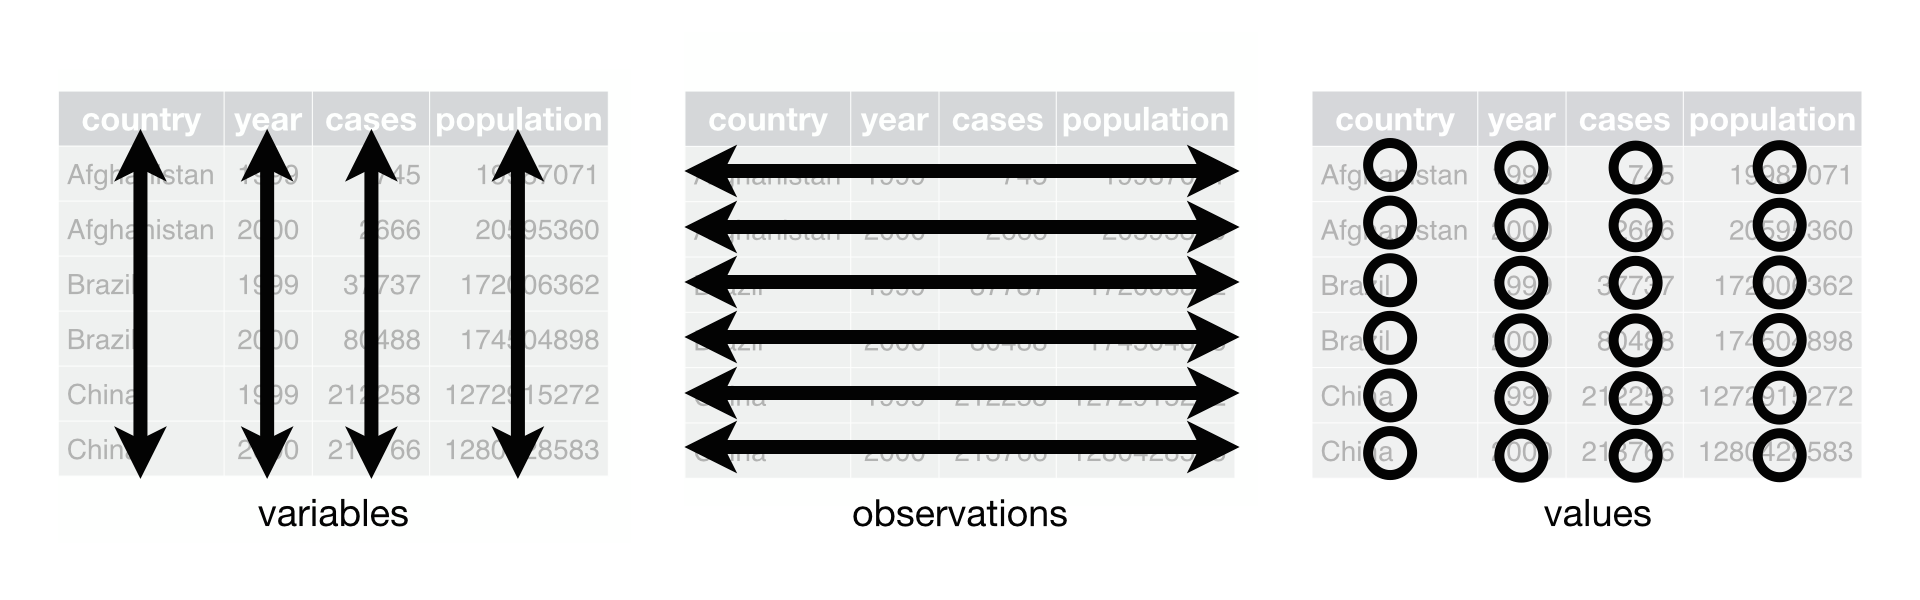
\includegraphics[width=500px]{images/tidy-data} 

}

\caption{The principles of tidy data}\label{fig:tidydata}
\end{figure}

Tidy data have two main advantages:

\begin{enumerate}
\def\labelenumi{\arabic{enumi}.}
\tightlist
\item
  There's a general advantage to picking one consistent way of storing data. If you have a consistent data structure, it's easier to learn the tools that work with it because they have an underlying uniformity.
\item
  There's a specific advantage to placing variables in columns because it allows you to easily access the columns in \emph{R} with the \texttt{\$} operation and the great functions of \emph{Tidyverse} as you have seen above.
\end{enumerate}

This means for most real analyses, you'll need to do some reshaping of the data and you have to go through the following two steps

\begin{enumerate}
\def\labelenumi{\arabic{enumi}.}
\tightlist
\item
  Figure out what the variables and observations or cases are.
\item
  You have to clean up the messy data structure and resolve at least one of the two common problems:

  \begin{enumerate}
  \def\labelenumii{\alph{enumii}.}
  \tightlist
  \item
    One variable might be spread across multiple columns.
  \item
    One observation might be scattered across multiple rows.
  \end{enumerate}
\end{enumerate}

\subsection{Long and Wide Data}\label{long-and-wide-data}

Tidy data can be organized in different ways. A common problem is for instance that you can treat different measurements as either

\begin{itemize}
\tightlist
\item
  different variables or
\item
  as the same variable under different condition.
\end{itemize}

That is, sometimes it's not easy the say what the columns/variables in your dataset really should be.
fig
In data science, we distinguish between long and wide data structures. Let's have a look at an example. The dataset \texttt{weight} comprises the weights for four overweighted subjects before and after a diet and their age. There are two representations of the same data possible:

\begin{table}
\caption{\label{tab:longwide} The same tidy data structures in a wide (left) or long (right) format.}

\begin{longtable}[t]{lrrr}
\toprule
Subject & Age & Before & After\\
\midrule
Peter & 23 & 105.0 & 98.5\\
Frank & 29 & 102.5 & 97.5\\
Bob & 34 & 96.5 & 95.5\\
Jim & 25 & 91.0 & 87.0\\
\bottomrule
\end{longtable}
\begin{longtable}[t]{lrlr}
\toprule
Subject & Age & Time & Weight\\
\midrule
Peter & 23 & Before & 105.0\\
Peter & 23 & After & 98.5\\
Frank & 29 & Before & 102.5\\
Frank & 29 & After & 97.5\\
Bob & 34 & Before & 96.5\\
\addlinespace
Bob & 34 & After & 95.5\\
Jim & 25 & Before & 91.0\\
Jim & 25 & After & 87.0\\
\bottomrule
\end{longtable}
\end{table}

As you see in the \textbf{long data} format at the \textbf{right}, the time is coded as a variable and gets thus it's own column. If you intend to do, for instance, a one-way factorial ANOVA with the independent variable \texttt{time} and the dependent variable \texttt{weight}, this long format directly illustrates the involved variables or factors (IV \& DV). And in fact, most functions that do inferential statistics in \emph{R} require this type of long data representation (e.g., the package \texttt{afex} for ANVOAs).

In contrast, in the \textbf{wide data} format at the \textbf{left} all measurements that belong to one person/case get their variable (in our example, \texttt{before} and \texttt{after}). One person/case is not spread across multiple rows. \emph{SPSS} uses, for instance, this representations and needs always a \emph{wide format} for all repeated measurements. That is, a wide data format represents all repeated measurements of the same person/case (such as weight at time 1 \& 2) in different columns/variables. Only between subject variables, such as the \texttt{age}, get in the wide data format it's own column. By the way: also the \emph{t}-test function in \emph{R} (\texttt{t-test()}) needs a wide data format.

\subsubsection{Pivoting functions}\label{pivoting-functions}

\emph{Tidyverse} offers the functions \texttt{pivot\_longer()} and \texttt{pivot\_wider()} to convert data between the two formats. For example, the file \texttt{weight.csv} \href{./data}{data folder} contains the data above in the wide data format (left part of Table \ref{tab:longwide}).

\begin{Shaded}
\begin{Highlighting}[]
\NormalTok{weight }\OtherTok{\textless{}{-}} \FunctionTok{read\_csv}\NormalTok{(}\StringTok{"data/weight.csv"}\NormalTok{)}
\FunctionTok{print}\NormalTok{(weight)}
\end{Highlighting}
\end{Shaded}

\begin{verbatim}
## # A tibble: 4 x 4
##   Subject   Age Before After
##   <chr>   <dbl>  <dbl> <dbl>
## 1 Peter      23  105    98.5
## 2 Frank      29  102.   97.5
## 3 Bob        34   96.5  95.5
## 4 Jim        25   91    87
\end{verbatim}

\paragraph*{Wide to long}\label{wide-to-long}
\addcontentsline{toc}{paragraph}{Wide to long}

It's simple and straightforward to covert the wide data to a long format:

\begin{Shaded}
\begin{Highlighting}[]
\NormalTok{weight\_long }\OtherTok{\textless{}{-}} \FunctionTok{pivot\_longer}\NormalTok{(weight, }\FunctionTok{c}\NormalTok{(}\StringTok{"Before"}\NormalTok{, }\StringTok{"After"}\NormalTok{), }\AttributeTok{names\_to=}\StringTok{"Time"}\NormalTok{, }\AttributeTok{values\_to=}\StringTok{"Weight"}\NormalTok{)}
\end{Highlighting}
\end{Shaded}

Please note, the second argument of \texttt{pivot\_longer()} is the columns to be rearranged and has to be a vector of the names (\texttt{c(...)}). The single names of the columns have to be in quotes (\texttt{"..."}). The resulting data frame is now in long format:

\begin{Shaded}
\begin{Highlighting}[]
\FunctionTok{print}\NormalTok{(weight\_long)}
\end{Highlighting}
\end{Shaded}

\begin{verbatim}
## # A tibble: 8 x 4
##   Subject   Age Time   Weight
##   <chr>   <dbl> <chr>   <dbl>
## 1 Peter      23 Before  105  
## 2 Peter      23 After    98.5
## 3 Frank      29 Before  102. 
## 4 Frank      29 After    97.5
## 5 Bob        34 Before   96.5
## 6 Bob        34 After    95.5
## 7 Jim        25 Before   91  
## 8 Jim        25 After    87
\end{verbatim}

\paragraph*{Long to wide}\label{long-to-wide}
\addcontentsline{toc}{paragraph}{Long to wide}

The function \texttt{pivot\_wider()} does the opposite, that is, it transforms a long data format into a wide format.

\begin{myexercise}
Try to figure out how \texttt{pivot\_wider()} works and use this
function to convert the data frame \texttt{weight\_long} back to a wide
format.
\end{myexercise}
\webexhide{Solution}

\begin{Shaded}
\begin{Highlighting}[]
\NormalTok{wide\_again }\OtherTok{\textless{}{-}} \FunctionTok{pivot\_wider}\NormalTok{(weight\_long, }\AttributeTok{names\_from=}\StringTok{"Time"}\NormalTok{, }\AttributeTok{values\_from=}\StringTok{"Weight"}\NormalTok{)}
\FunctionTok{print}\NormalTok{(wide\_again)}
\end{Highlighting}
\end{Shaded}

\begin{verbatim}
## # A tibble: 4 x 4
##   Subject   Age Before After
##   <chr>   <dbl>  <dbl> <dbl>
## 1 Peter      23  105    98.5
## 2 Frank      29  102.   97.5
## 3 Bob        34   96.5  95.5
## 4 Jim        25   91    87
\end{verbatim}

\webexunhide

Hint: Further information about pivoting can be found in the build-in help of \emph{R} if you type \texttt{vignette("pivot")} and look at the help panel in RStudio.

\begin{geek}
Old versions of \emph{Tidyverse} (\textless1.0) don't have this pivoting
functions and used instead the functions \texttt{gather()}and
\texttt{spread()}. The old functions still work, but I suggest to use
the new \texttt{pivot\_wider()} and \texttt{pivot\_longer()} functions.
\end{geek}

\newpage

\part{Data Processing \& Visualizing}\label{part-data-processing-visualizing}

\section{Missing Values}\label{missing-values}

\emph{R} has a distinct data type to indicate that an object, a variable or aN element of a vector has no value or that this data point is missing.

\subsection{\texorpdfstring{\texttt{NA}: Not Available}{NA: Not Available}}\label{na-not-available}

\texttt{NA} stands for ``Not Available'' and is used to indicate a missing value. For instance, if you have a vector of the body heights of three subjects and, let's say, you don't know the height of the second person, it should look like this in \emph{R}:

\begin{Shaded}
\begin{Highlighting}[]
\NormalTok{height }\OtherTok{=} \FunctionTok{c}\NormalTok{(}\FloatTok{1.69}\NormalTok{, }\ConstantTok{NA}\NormalTok{, }\FloatTok{1.82}\NormalTok{)}
\end{Highlighting}
\end{Shaded}

Importantly, \textbf{any operation and any comparison with\texttt{NA} has the result \texttt{NA}}. That is, if you make an element-wise operation or comparison with the vector, \emph{R} returns always \texttt{NA} for any missing elements.

\begin{Shaded}
\begin{Highlighting}[]
\NormalTok{height }\SpecialCharTok{*} \DecValTok{100}  \CommentTok{\# height in cm}
\end{Highlighting}
\end{Shaded}

\begin{verbatim}
## [1] 169  NA 182
\end{verbatim}

\begin{Shaded}
\begin{Highlighting}[]
\NormalTok{large\_guys }\OtherTok{=}\NormalTok{ height }\SpecialCharTok{\textgreater{}} \FloatTok{1.80}  \CommentTok{\# find all the large guys}
\FunctionTok{print}\NormalTok{(large\_guys)}
\end{Highlighting}
\end{Shaded}

\begin{verbatim}
## [1] FALSE    NA  TRUE
\end{verbatim}

If you want to figure out which elements in a vector is \texttt{NA}, you have to use \texttt{is.na()} function:

\begin{Shaded}
\begin{Highlighting}[]
\FunctionTok{is.na}\NormalTok{(height)}
\end{Highlighting}
\end{Shaded}

\begin{verbatim}
## [1] FALSE  TRUE FALSE
\end{verbatim}

Since your use the \texttt{!}-sign in \emph{R} to make a negation (like in the comparison \emph{``is not equal''} \texttt{!=}; see section \ref{logicals} about logicals or section \ref{comparing} about comparisons), you can use this to find all elements in a vector that are \textbf{NOT} \texttt{NA}:

\begin{Shaded}
\begin{Highlighting}[]
\SpecialCharTok{!}\FunctionTok{is.na}\NormalTok{(height)}
\end{Highlighting}
\end{Shaded}

\begin{verbatim}
## [1]  TRUE FALSE  TRUE
\end{verbatim}

\paragraph*{Aggregating/processing vectors with missing values}\label{aggregatingprocessing-vectors-with-missing-values}
\addcontentsline{toc}{paragraph}{Aggregating/processing vectors with missing values}

Since all operations with missing values return \texttt{NA}, all functions that calculate a single value from a vector (e.g.~\texttt{sum()}, \texttt{mean()} or \texttt{sd()}) return always \texttt{NA}, if only one single value in the vector is \texttt{NA}.

\begin{Shaded}
\begin{Highlighting}[]
\FunctionTok{mean}\NormalTok{(height)}
\end{Highlighting}
\end{Shaded}

\begin{verbatim}
## [1] NA
\end{verbatim}

That is a problem, because we typically just want to ignore \texttt{NA} and calculate the results without the missing value. To do so, we have to exclude all \texttt{NA} values. We could do this manually by selecting only the elements that are not \texttt{NA} (e.g.~using \texttt{filter()} or base-\emph{R} \url{subsetting}). However, most vector-base functions in \emph{R} offer the option to remove all \texttt{NA}s. This option is called \texttt{na.rm=} and if it's set to \texttt{TRUE}, \emph{R} excludes the \texttt{NA} before doing the calculation:

\begin{Shaded}
\begin{Highlighting}[]
\FunctionTok{mean}\NormalTok{(height, }\AttributeTok{na.rm =} \ConstantTok{TRUE}\NormalTok{)}
\end{Highlighting}
\end{Shaded}

\begin{verbatim}
## [1] 1.755
\end{verbatim}

\webexhide{manually deleting NA}

\begin{Shaded}
\begin{Highlighting}[]
\CommentTok{\# manually deleting  NA}
\FunctionTok{mean}\NormalTok{(height[}\SpecialCharTok{!}\FunctionTok{is.na}\NormalTok{(height)])}
\end{Highlighting}
\end{Shaded}

\begin{verbatim}
## [1] 1.755
\end{verbatim}

\begin{Shaded}
\begin{Highlighting}[]
\CommentTok{\# but this is easier, right?}
\FunctionTok{mean}\NormalTok{(height, }\AttributeTok{na.rm =} \ConstantTok{TRUE}\NormalTok{)}
\end{Highlighting}
\end{Shaded}

\begin{verbatim}
## [1] 1.755
\end{verbatim}

\webexunhide

\subsection{Missings in data frames}\label{missings-in-data-frames}

The datasets that we have used in the previous chapter were always complete and did not contain any missing data point. In real life, however, you often encounter the situation that you are missing some measurements in some variables. In other words, not all subjects provide a measurement in all columns. This might cause problems for the data processing and we need to deal with that issue.

The \href{./data}{data folder} contains a second (more realistic) version of the teaching method dataset called \texttt{teaching\_method2.csv}. Let's have a look at it.

\begin{Shaded}
\begin{Highlighting}[]
\NormalTok{teach }\OtherTok{\textless{}{-}} \FunctionTok{read\_csv}\NormalTok{(}\StringTok{"data/teaching\_method2.csv"}\NormalTok{)}
\FunctionTok{summary}\NormalTok{(teach)}
\end{Highlighting}
\end{Shaded}

\begin{verbatim}
##     student     teaching_method        city               time          
##  Min.   : 1.0   Length:60          Length:60          Length:60         
##  1st Qu.: 8.0   Class :character   Class :character   Class :character  
##  Median :15.5   Mode  :character   Mode  :character   Mode  :character  
##  Mean   :15.5                                                           
##  3rd Qu.:23.0                                                           
##  Max.   :30.0                                                           
##                                                                         
##    statistics       cog_psy     
##  Min.   : 4.00   Min.   : 5.00  
##  1st Qu.: 9.00   1st Qu.:10.00  
##  Median :12.00   Median :12.00  
##  Mean   :15.39   Mean   :18.41  
##  3rd Qu.:23.00   3rd Qu.:31.00  
##  Max.   :37.00   Max.   :40.00  
##  NA's   :3       NA's   :2
\end{verbatim}

As you see in the summary, we have 3 missing values the variable \texttt{statistics} and \texttt{cog\_psy}. In the data viewer it look like this.

\begin{figure}

{\centering 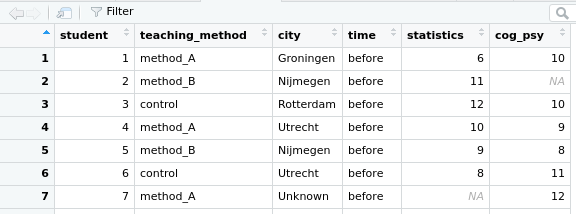
\includegraphics[width=500px]{images/missings_unknown} 

}

\caption{Screen shot of the data frame displayed in RStudio Viewer}\label{fig:missingsscreenshort}
\end{figure}

\begin{myexercise}
Calculate the mean of \texttt{statistics} and \texttt{cog\_psy} using
the \texttt{summarise()} function of \emph{Tidyverse}?
\end{myexercise}
\webexhide{Solution}

\begin{Shaded}
\begin{Highlighting}[]
\FunctionTok{summarise}\NormalTok{(teach, }\AttributeTok{m\_stats =} \FunctionTok{mean}\NormalTok{(statistics, }\AttributeTok{na.rm=}\ConstantTok{TRUE}\NormalTok{),}
          \AttributeTok{m\_cog\_psy =} \FunctionTok{mean}\NormalTok{(cog\_psy, }\AttributeTok{na.rm=}\ConstantTok{TRUE}\NormalTok{))}
\end{Highlighting}
\end{Shaded}

\begin{verbatim}
## # A tibble: 1 x 2
##   m_stats m_cog_psy
##     <dbl>     <dbl>
## 1    15.4      18.4
\end{verbatim}

\webexunhide

\subsubsection{Defining missing values}\label{defining-missing-values}

As you have seen above, when using \texttt{read\_csv()}, \emph{R} detected automatically the missing values in the variables \texttt{statistics} and \texttt{cog\_psy} and inserted instead \texttt{NA}. This was the case because there was simple no value in the data file.

However, very often scientist use specific values to indicate in their raw data that there is a missing value (e.g.~\texttt{??}, \texttt{None}, \texttt{Missing}, \texttt{-99}). For example, if you look carefully on the screenshot of the data viewer above (figure \ref{fig:missingsscreenshort}), the \texttt{city} in row 7 is \emph{``Unknown''}, which is obviously a missing value. \emph{R} doesn't know that, of course, and we have to indicate that the data point \emph{``Unknown''} represents a missing values and not a Dutch city.

Data reading functions have the optional argument \texttt{na}, which calls for a vector of the values/labels that are representing missing values in this dataset. For example:

\begin{Shaded}
\begin{Highlighting}[]
\NormalTok{teach }\OtherTok{\textless{}{-}} \FunctionTok{read\_csv}\NormalTok{(}\StringTok{"data/teaching\_method2.csv"}\NormalTok{, }\AttributeTok{na =} \FunctionTok{c}\NormalTok{(}\StringTok{"Unknown"}\NormalTok{))}
\end{Highlighting}
\end{Shaded}

As you see, city in row 7 is now a missing.

\begin{figure}

{\centering 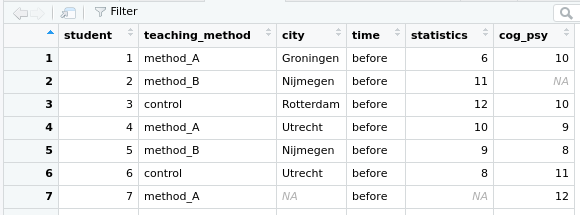
\includegraphics[width=500px]{images/missings} 

}

\caption{Screen shot of the data frame displayed in RStudio Viewer. 'Unknown' is now defined as missing.}\label{fig:unnamed-chunk-210}
\end{figure}

If you have multiple values that represent a missing value, it could look like this:

\begin{Shaded}
\begin{Highlighting}[]
\NormalTok{df }\OtherTok{\textless{}{-}} \FunctionTok{read\_csv}\NormalTok{(}\StringTok{"demo.csv"}\NormalTok{, }\AttributeTok{na =} \FunctionTok{c}\NormalTok{(}\StringTok{"Unknown"}\NormalTok{, }\StringTok{"??"}\NormalTok{, }\StringTok{"None"}\NormalTok{, }\SpecialCharTok{{-}}\DecValTok{99}\NormalTok{,  }\StringTok{"no idea"}\NormalTok{, }\StringTok{"who knows"}\NormalTok{))}
\end{Highlighting}
\end{Shaded}

\subsubsection{Drop rows with missing values}\label{drop-rows-with-missing-values}

\emph{Tidyverse} has the function \texttt{drop\_na()} to remove rows from a data frame that contain missing values. This command excludes all(!) rows, in which one or more variables are \texttt{NA}:

\begin{Shaded}
\begin{Highlighting}[]
\NormalTok{teach\_no\_na }\OtherTok{\textless{}{-}} \FunctionTok{drop\_na}\NormalTok{(teach)}
\end{Highlighting}
\end{Shaded}

Often you only want to remove rows, in which only certain variables are \texttt{NA}. Like in all \emph{Tidyverse} functions, you can specify variables to which it a certain operations should be apply. For instance, if you want to remove all rows in which the variables \texttt{city} or \texttt{statistics} are \texttt{NA}.

\begin{Shaded}
\begin{Highlighting}[]
\FunctionTok{drop\_na}\NormalTok{(teach, city, statistics)}
\end{Highlighting}
\end{Shaded}

\begin{myexercise}
Calculate the again mean of \texttt{statistics} and \texttt{cog\_psy}
with \texttt{summarise()}, but this time use also \texttt{drop\_na()}?
Try to do it in one line of code.
\end{myexercise}
\webexhide{Solution}

\begin{Shaded}
\begin{Highlighting}[]
\FunctionTok{summarise}\NormalTok{(}\FunctionTok{drop\_na}\NormalTok{(teach), }\AttributeTok{m\_stats =} \FunctionTok{mean}\NormalTok{(statistics),}
          \AttributeTok{m\_cog\_psy =} \FunctionTok{mean}\NormalTok{(cog\_psy))}
\end{Highlighting}
\end{Shaded}

\begin{verbatim}
## # A tibble: 1 x 2
##   m_stats m_cog_psy
##     <dbl>     <dbl>
## 1    15.6      18.4
\end{verbatim}

\webexunhide

\subsubsection{Replacing missing values}\label{replacing-missing-values}

If we know that a missing value in a certain variable actually stands for an particular meaningful value, we can replace all \texttt{NA}s values in that variable by using \texttt{mutate()} and \texttt{replace\_na()}-function:

\begin{Shaded}
\begin{Highlighting}[]
\NormalTok{teach }\OtherTok{\textless{}{-}} \FunctionTok{mutate}\NormalTok{(teach,}
              \AttributeTok{city =} \FunctionTok{replace\_na}\NormalTok{(city, }\StringTok{"Amsterdam"}\NormalTok{))}
\end{Highlighting}
\end{Shaded}

This replaces all missing values in the variable with \emph{``Amsterdam''}. However, be careful and use \texttt{replace\_na()} only, if you are absolutely sure that you can replace the missing values without messing up your data.

\section{Factors}\label{factors}

In \emph{R} , factors are used to work with categorical variables. A categorical variable are often represented as text variables in raw data files (e.g.~the words \emph{``Male''} or \emph{``Female''}).

\begin{important}
A factor is defined as a variable that has a \emph{\emph{fixed}} and
\textbf{known} set of possible values or factor levels.
\end{important}

\subsection{Creating factors}\label{creating-factors}

Examples of categorical factors are the variables \texttt{teaching\_method}, \texttt{time} and \texttt{city} in our dataset \texttt{teaching\_method2.csv}. You see that the variables are character variables \texttt{\textless{}chr\textgreater{}} when reading the CSV-file into \emph{R}.

\begin{Shaded}
\begin{Highlighting}[]
\NormalTok{teach }\OtherTok{\textless{}{-}} \FunctionTok{read\_csv}\NormalTok{(}\StringTok{"data/teaching\_method2.csv"}\NormalTok{, }\AttributeTok{na =} \FunctionTok{c}\NormalTok{(}\StringTok{"Unknown"}\NormalTok{))}
\FunctionTok{glimpse}\NormalTok{(teach)}
\end{Highlighting}
\end{Shaded}

\begin{verbatim}
## Rows: 60
## Columns: 6
## $ student         <dbl> 1, 2, 3, 4, 5, 6, 7, 8, 9, 10, 11, 12, 13, 14, 15, 16,~
## $ teaching_method <chr> "method_A", "method_B", "control", "method_A", "method~
## $ city            <chr> "Groningen", "Nijmegen", "Rotterdam", "Utrecht", "Nijm~
## $ time            <chr> "before", "before", "before", "before", "before", "bef~
## $ statistics      <dbl> 6, 11, 12, 10, 9, 8, NA, 9, 8, 10, 16, 11, 8, 12, 13, ~
## $ cog_psy         <dbl> 10, NA, 10, 9, 8, 11, 12, 12, 10, 12, 8, 13, 13, 8, 10~
\end{verbatim}

We want to treat these variable as factors, because they have a fixed and known number of factor levels. To tell \emph{R} that variables in a data frame (or tibble) are factors, we make use of the function \texttt{factor()} and \texttt{mutate()} to `replace' a particular text variable with a factor representation of this variable:

\begin{Shaded}
\begin{Highlighting}[]
\NormalTok{teach\_with\_factors }\OtherTok{\textless{}{-}} \FunctionTok{mutate}\NormalTok{(teach,}
                       \AttributeTok{teaching\_method=}\FunctionTok{factor}\NormalTok{(teaching\_method),}
                       \AttributeTok{city=}\FunctionTok{factor}\NormalTok{(city),}
                       \AttributeTok{time=}\FunctionTok{factor}\NormalTok{(time))}
\FunctionTok{glimpse}\NormalTok{(teach\_with\_factors)}
\end{Highlighting}
\end{Shaded}

\begin{verbatim}
## Rows: 60
## Columns: 6
## $ student         <dbl> 1, 2, 3, 4, 5, 6, 7, 8, 9, 10, 11, 12, 13, 14, 15, 16,~
## $ teaching_method <fct> method_A, method_B, control, method_A, method_B, contr~
## $ city            <fct> Groningen, Nijmegen, Rotterdam, Utrecht, Nijmegen, Utr~
## $ time            <fct> before, before, before, before, before, before, before~
## $ statistics      <dbl> 6, 11, 12, 10, 9, 8, NA, 9, 8, 10, 16, 11, 8, 12, 13, ~
## $ cog_psy         <dbl> 10, NA, 10, 9, 8, 11, 12, 12, 10, 12, 8, 13, 13, 8, 10~
\end{verbatim}

The three variables are now factors (\texttt{\textless{}fct\textgreater{}}). The same could be achieved with base-\emph{R}, but it is less convenient.

\webexhide{Making factors with base-R is less readable}

\begin{Shaded}
\begin{Highlighting}[]
\NormalTok{teach\_with\_factors }\OtherTok{\textless{}{-}}\NormalTok{ teach}
\NormalTok{teach\_with\_factors}\SpecialCharTok{$}\NormalTok{teaching\_method }\OtherTok{=} \FunctionTok{factor}\NormalTok{(teach\_with\_factors}\SpecialCharTok{$}\NormalTok{teaching\_method)}
\NormalTok{teach\_with\_factors}\SpecialCharTok{$}\NormalTok{city }\OtherTok{=} \FunctionTok{factor}\NormalTok{(teach\_with\_factors}\SpecialCharTok{$}\NormalTok{city)}
\NormalTok{teach\_with\_factors}\SpecialCharTok{$}\NormalTok{time }\OtherTok{=} \FunctionTok{factor}\NormalTok{(teach\_with\_factors}\SpecialCharTok{$}\NormalTok{time)}
\end{Highlighting}
\end{Shaded}

\webexunhide

\subsection{Advantages of factors}\label{advantages-of-factors}

The Advantages of using factors can be best illustrated with a typical example of a categorical variable in psychology: the \emph{gender}. People often use numbers to code to genders and enter for instance for the females \texttt{1} and males with \texttt{2}.

\begin{Shaded}
\begin{Highlighting}[]
\NormalTok{df\_no\_factor }\OtherTok{=} \FunctionTok{data.frame}\NormalTok{(}\AttributeTok{gender=}\FunctionTok{c}\NormalTok{(}\DecValTok{1}\NormalTok{,}\DecValTok{2}\NormalTok{,}\DecValTok{3}\NormalTok{,}\DecValTok{2}\NormalTok{,}\DecValTok{1}\NormalTok{, }\DecValTok{1}\NormalTok{,}\DecValTok{2}\NormalTok{,}\DecValTok{2}\NormalTok{,}\DecValTok{2}\NormalTok{,}\DecValTok{1}\NormalTok{))}
\FunctionTok{print}\NormalTok{(df\_no\_factor)}
\end{Highlighting}
\end{Shaded}

\begin{verbatim}
##    gender
## 1       1
## 2       2
## 3       3
## 4       2
## 5       1
## 6       1
## 7       2
## 8       2
## 9       2
## 10      1
\end{verbatim}

\subsubsection{Predefined factor levels}\label{predefined-factor-levels}

One advantage of factors is that you can define the possible factor levels (like \texttt{...,levels=c(1,\ 2),...}) and when an row/observation has a values that does not fit the predefined levels, the values will be set automatically to \texttt{NA}. You can do it with the function argument \texttt{levels} .

\begin{Shaded}
\begin{Highlighting}[]
\NormalTok{df\_factor }\OtherTok{\textless{}{-}}  \FunctionTok{mutate}\NormalTok{(df\_no\_factor,}
            \AttributeTok{gender =} \FunctionTok{factor}\NormalTok{(gender, }\AttributeTok{levels=}\FunctionTok{c}\NormalTok{(}\DecValTok{1}\NormalTok{, }\DecValTok{2}\NormalTok{)))}
\FunctionTok{print}\NormalTok{(df\_factor)}
\end{Highlighting}
\end{Shaded}

\begin{verbatim}
##    gender
## 1       1
## 2       2
## 3    <NA>
## 4       2
## 5       1
## 6       1
## 7       2
## 8       2
## 9       2
## 10      1
\end{verbatim}

Gender \texttt{3} became not not \texttt{NA}.

\subsubsection{Meaningful factor labels}\label{meaningful-factor-labels}

You can introduce useful factor labels (or descriptions) for each level, which make your analysis script and, importantly, the produced output more readable and more transparent.

Don't forget, often the factor levels are represented in a raw data file just by codes. This data is not self-explaining and I'm sure that you can't remember in a few weeks whether the females or the males have the value \texttt{1}. I therefore \textbf{strongly} suggest to add self-explaining labels for all levels of the factor. You can do it with the function argument \texttt{labels}.

\begin{Shaded}
\begin{Highlighting}[]
\NormalTok{df\_factor }\OtherTok{\textless{}{-}}  \FunctionTok{mutate}\NormalTok{(df\_no\_factor,}
            \AttributeTok{gender =} \FunctionTok{factor}\NormalTok{(gender, }\AttributeTok{levels=}\FunctionTok{c}\NormalTok{(}\DecValTok{1}\NormalTok{, }\DecValTok{2}\NormalTok{), }\AttributeTok{labels=}\FunctionTok{c}\NormalTok{(}\StringTok{"female"}\NormalTok{, }\StringTok{"male"}\NormalTok{)))}
\FunctionTok{print}\NormalTok{(df\_factor)}
\end{Highlighting}
\end{Shaded}

\begin{verbatim}
##    gender
## 1  female
## 2    male
## 3    <NA>
## 4    male
## 5  female
## 6  female
## 7    male
## 8    male
## 9    male
## 10 female
\end{verbatim}

\subsubsection{Statistics with categorical variables}\label{statistics-with-categorical-variables}

Inferential statistics needs to know which variable is categorical and which is continuous. Almost all packages that do inferential statistics (see \hyperref[packagelist]{Appendix} \ref{packagelist}) use factors to indicate categorical variables.

\subsubsection{Nice output}\label{nice-output}

The output of some functions is nicer and better organized. If we do a summary of the data frame without factors:

\begin{Shaded}
\begin{Highlighting}[]
\FunctionTok{summary}\NormalTok{(df\_no\_factor)}
\end{Highlighting}
\end{Shaded}

\begin{verbatim}
##      gender   
##  Min.   :1.0  
##  1st Qu.:1.0  
##  Median :2.0  
##  Mean   :1.7  
##  3rd Qu.:2.0  
##  Max.   :3.0
\end{verbatim}

and with factors,

\begin{Shaded}
\begin{Highlighting}[]
\FunctionTok{summary}\NormalTok{(df\_factor)}
\end{Highlighting}
\end{Shaded}

\begin{verbatim}
##     gender 
##  female:4  
##  male  :5  
##  NA's  :1
\end{verbatim}

you see that only the summary of the factor gender is meaningful and it provide is need information of all factor levels and amount of observations in each level.

\begin{geek}
Factors are also very useful when you need to display or process
character variables in a predefined non-alphabetical order, for
instance,
\texttt{c("Mon",\ "Tue",\ "Wed",\ "Thr",\ "Fri",\ "Sat",\ "Son")}.
However, this aspect is less relevant for social sciences and it will be
therefore not disccused here. (but see for instance
\href{https://r4ds.had.co.nz/factors.html\#introduction-9}{this
tutorial} or the documentation of factors in \emph{Tidyverse}, the
\href{https://forcats.tidyverse.org/}{forcats package}).
\end{geek}

\section{Pipes}\label{pipes}

You have seen in the previous chapters that if you have a raw dataset you need to apply typically multiple operations and processing steps on a dataset. The resulting data of one operations, will be used a input data for the next operations. That is, when processing and analysing data, we typically setup a processing pipeline.

\begin{center}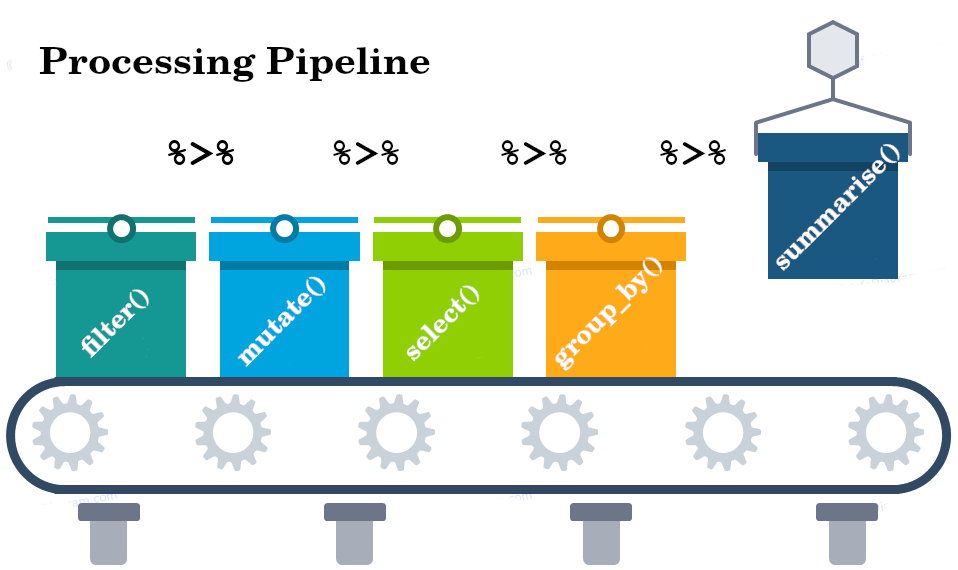
\includegraphics[width=500px]{images/pipeline} \end{center}

Pipes are a powerful tool for clearly expressing a sequence of multiple operations. Pipes are a way to order your code in a more readable format.

\subsection{\texorpdfstring{The pipe operator: \texttt{\%\textgreater{}\%}}{The pipe operator: \%\textgreater\%}}\label{the-pipe-operator}

\emph{Tidyverse} has the operator \texttt{\%\textgreater{}\%}, which sends an object (e.g.~data frame) as input for the following function:

For example, instead writing

\begin{Shaded}
\begin{Highlighting}[]
\CommentTok{\# classical function call}
\FunctionTok{drop\_na}\NormalTok{(my\_data)                }\CommentTok{\# example a}
\FunctionTok{mutate}\NormalTok{(my\_data, }\AttributeTok{new\_var =}\NormalTok{ a }\SpecialCharTok{+}\NormalTok{ b) }\CommentTok{\# example b}
\end{Highlighting}
\end{Shaded}

you can write

\begin{Shaded}
\begin{Highlighting}[]
\CommentTok{\# the same with pipes}
\NormalTok{my\_data }\SpecialCharTok{\%\textgreater{}\%} \FunctionTok{drop\_na}\NormalTok{()                }\CommentTok{\# example a}
\NormalTok{my\_data }\SpecialCharTok{\%\textgreater{}\%} \FunctionTok{mutate}\NormalTok{(}\AttributeTok{new\_var =}\NormalTok{ a }\SpecialCharTok{+}\NormalTok{ b)  }\CommentTok{\# example b}
\end{Highlighting}
\end{Shaded}

The two versions of example a and b do exactly the same. It's just a different syntax. Instead having the data frame as first argument of the functions \texttt{drop\_na()} or \texttt{mutate()} (first two example lines), you ``push it'' or ``pipe it'' to the following function with \texttt{\%\textgreater{}\%}. That is, \emph{R} uses the forwarded object as input for function and you can (or have to!) omit mentioning the data inside the function call (last two example lines).

\begin{geek}
The package that defines pipes in \emph{Tidyverse} is called
\texttt{magrittr}.
\end{geek}

\subsection{Motivation for pipes}\label{motivation-for-pipes}

Why shall I use pipes? Pipes can be very handy, because you can not only send data to functions, but also the results of functions (i.e., the resulting data) to the following functions. You can build with this technology very efficiently a complex processing pipeline and your code remains well structured and readable (which this is always the aim of a good data science practice).

\begin{Shaded}
\begin{Highlighting}[]
\CommentTok{\# classical function call}
\NormalTok{data\_with\_na }\OtherTok{\textless{}{-}} \FunctionTok{drop\_na}\NormalTok{(my\_data)                }\CommentTok{\# step a}
\FunctionTok{mutate}\NormalTok{(data\_with\_na, }\AttributeTok{new\_var =}\NormalTok{ a }\SpecialCharTok{+}\NormalTok{ b) }\CommentTok{\# step b}

\CommentTok{\# the same with pipes}
\NormalTok{my\_data }\SpecialCharTok{\%\textgreater{}\%} \FunctionTok{drop\_na}\NormalTok{() }\SpecialCharTok{\%\textgreater{}\%} \FunctionTok{mutate}\NormalTok{(}\AttributeTok{new\_var =}\NormalTok{ a }\SpecialCharTok{+}\NormalTok{ b)  }\CommentTok{\# step a and b}
\end{Highlighting}
\end{Shaded}

\begin{important}
 Don't forget, pipes work only with functions that are developed for this
 purpose. Fortunately, this is the case for all
 \emph{Tidyverse}-functions.
 \end{important}

\subsection{Building a processing pipeline}\label{building-a-processing-pipeline}

Let's have an example and use our dataset \texttt{teaching\_method2.csv} (see section \ref{transformingdata}). Assume we want to calculate the mean percent correct in cognitive psychology for all cities and teaching methods. We want also to exclude the cities \emph{``Leiden''} and \emph{``Utrecht''}. You know we have missing values and need to deal with it.

\begin{myexercise}
Try to do this analysis yourself, be fore you go on.
\end{myexercise}

\subsubsection{Intermediate steps}\label{intermediatesteps}

To do it, we need to read the data and process it in multiple steps. For each step we create a new data frame and use the previous data frame as input. You are already familiar with that approach.

One solution to the problem above looks, for example, like this:

\begin{Shaded}
\begin{Highlighting}[]
\CommentTok{\#reading the data}
\NormalTok{teach }\OtherTok{\textless{}{-}} \FunctionTok{read\_csv}\NormalTok{(}\StringTok{"data/teaching\_method2.csv"}\NormalTok{, }\AttributeTok{na =} \FunctionTok{c}\NormalTok{(}\StringTok{"Unknown"}\NormalTok{))}
\end{Highlighting}
\end{Shaded}

\begin{Shaded}
\begin{Highlighting}[]
\CommentTok{\#remove nan values}
\NormalTok{teach2 }\OtherTok{\textless{}{-}} \FunctionTok{drop\_na}\NormalTok{(teach)}

\CommentTok{\# filtering the cities}
\NormalTok{teach3 }\OtherTok{\textless{}{-}} \FunctionTok{filter}\NormalTok{(teach2, city }\SpecialCharTok{!=} \StringTok{"Leiden"}\NormalTok{, city }\SpecialCharTok{!=} \StringTok{"Utrecht"}\NormalTok{)}

\CommentTok{\# calculating percent correct for cog.psy{-}}
\NormalTok{teach4 }\OtherTok{\textless{}{-}} \FunctionTok{mutate}\NormalTok{(teach3, }\AttributeTok{percent\_cog\_psy=}\NormalTok{ cog\_psy }\SpecialCharTok{*} \DecValTok{40}\SpecialCharTok{/}\DecValTok{100}\NormalTok{)}

\CommentTok{\# group data for city and teaching method}
\NormalTok{teach4\_grouped }\OtherTok{\textless{}{-}} \FunctionTok{group\_by}\NormalTok{(teach4, city, teaching\_method)}

\CommentTok{\# making the summary}
\NormalTok{summary\_df}\OtherTok{\textless{}{-}} \FunctionTok{summarise}\NormalTok{(teach4\_grouped,}
                        \AttributeTok{m\_cog\_psy =} \FunctionTok{mean}\NormalTok{(percent\_cog\_psy) )}
\end{Highlighting}
\end{Shaded}

We produced in total 6 data frames (\texttt{teach}, \texttt{teach2}, \texttt{teach3}, \texttt{teach4}, \texttt{teach4\_grouped}, \texttt{summary\_df}), but we are actually only interested in the last data frame, which look like this:

\begin{Shaded}
\begin{Highlighting}[]
\FunctionTok{print}\NormalTok{(summary\_df)}
\end{Highlighting}
\end{Shaded}

\begin{verbatim}
## # A tibble: 9 x 3
## # Groups:   city [3]
##   city      teaching_method m_cog_psy
##   <chr>     <chr>               <dbl>
## 1 Groningen control              4.4 
## 2 Groningen method_A             7.84
## 3 Groningen method_B             9   
## 4 Nijmegen  control              4.7 
## 5 Nijmegen  method_A             7.8 
## 6 Nijmegen  method_B             9.28
## 7 Rotterdam control              4.4 
## 8 Rotterdam method_A             9.4 
## 9 Rotterdam method_B             7.1
\end{verbatim}

All the other five intermediate data frames are not really wanted as result. This is very inefficient and occupies a lot of memory.

\subsubsection{Overwrite the original}\label{overwrite-the-original}

Instead of creating intermediate objects at each step, we could overwrite the original object:

\begin{Shaded}
\begin{Highlighting}[]
\NormalTok{teach }\OtherTok{\textless{}{-}} \FunctionTok{read\_csv}\NormalTok{(}\StringTok{"data/teaching\_method2.csv"}\NormalTok{, }\AttributeTok{na =} \FunctionTok{c}\NormalTok{(}\StringTok{"Unknown"}\NormalTok{))}
\NormalTok{teach }\OtherTok{\textless{}{-}} \FunctionTok{drop\_na}\NormalTok{(teach)}
\NormalTok{teach }\OtherTok{\textless{}{-}} \FunctionTok{filter}\NormalTok{(teach, city }\SpecialCharTok{!=} \StringTok{"Leiden"}\NormalTok{, city }\SpecialCharTok{!=} \StringTok{"Utrecht"}\NormalTok{)}
\NormalTok{teach }\OtherTok{\textless{}{-}} \FunctionTok{mutate}\NormalTok{(teach, }\AttributeTok{percent\_cog\_psy=}\NormalTok{ cog\_psy }\SpecialCharTok{*} \DecValTok{40}\SpecialCharTok{/}\DecValTok{100}\NormalTok{)}
\NormalTok{teach }\OtherTok{\textless{}{-}} \FunctionTok{group\_by}\NormalTok{(teach, city, teaching\_method)}
\NormalTok{teach }\OtherTok{\textless{}{-}} \FunctionTok{summarise}\NormalTok{(teach, }\AttributeTok{m\_cog\_psy =} \FunctionTok{mean}\NormalTok{(percent\_cog\_psy) )}
\end{Highlighting}
\end{Shaded}

This is less typing (and less thinking), so you're less likely to make mistakes. However, there are two problems:

\begin{enumerate}
\def\labelenumi{\arabic{enumi}.}
\tightlist
\item
  Debugging is painful: if you make a mistake you'll need to re-run the complete pipeline from the beginning.
\item
  The repetition of the object being transformed (we've written foo\_foo six times!) obscures what's changing on each line.
\end{enumerate}

\subsubsection{\texorpdfstring{Build a processing pipeline with pipe \texttt{\%\textgreater{}\%}}{Build a processing pipeline with pipe \%\textgreater\%}}\label{build-a-processing-pipeline-with-pipe}

Finally, we can use the pipe:

\begin{Shaded}
\begin{Highlighting}[]
\NormalTok{summary\_df }\OtherTok{\textless{}{-}} \FunctionTok{read\_csv}\NormalTok{(}\StringTok{"data/teaching\_method2.csv"}\NormalTok{, }\AttributeTok{na =} \FunctionTok{c}\NormalTok{(}\StringTok{"Unknown"}\NormalTok{)) }\SpecialCharTok{\%\textgreater{}\%}
        \FunctionTok{drop\_na}\NormalTok{() }\SpecialCharTok{\%\textgreater{}\%}
        \FunctionTok{filter}\NormalTok{(city }\SpecialCharTok{!=} \StringTok{"Leiden"}\NormalTok{, city }\SpecialCharTok{!=} \StringTok{"Utrecht"}\NormalTok{) }\SpecialCharTok{\%\textgreater{}\%}
        \FunctionTok{mutate}\NormalTok{(}\AttributeTok{percent\_cog\_psy=}\NormalTok{ cog\_psy }\SpecialCharTok{*} \DecValTok{40}\SpecialCharTok{/}\DecValTok{100}\NormalTok{) }\SpecialCharTok{\%\textgreater{}\%}
        \FunctionTok{group\_by}\NormalTok{(city, teaching\_method) }\SpecialCharTok{\%\textgreater{}\%}
        \FunctionTok{summarise}\NormalTok{(}\AttributeTok{m\_cog\_psy =} \FunctionTok{mean}\NormalTok{(percent\_cog\_psy) )}
\end{Highlighting}
\end{Shaded}

If you compare this code with the code in which we produced multiple \hyperref[intermediatesteps]{intermediate data frames}, I think you see the benefit. It does not only do the same computations, it's also faster executed (which you noticed however only if you have really big datasets).

\begin{Shaded}
\begin{Highlighting}[]
\FunctionTok{print}\NormalTok{(summary\_df)}
\end{Highlighting}
\end{Shaded}

\begin{verbatim}
## # A tibble: 9 x 3
## # Groups:   city [3]
##   city      teaching_method m_cog_psy
##   <chr>     <chr>               <dbl>
## 1 Groningen control              4.4 
## 2 Groningen method_A             7.84
## 3 Groningen method_B             9   
## 4 Nijmegen  control              4.7 
## 5 Nijmegen  method_A             7.8 
## 6 Nijmegen  method_B             9.28
## 7 Rotterdam control              4.4 
## 8 Rotterdam method_A             9.4 
## 9 Rotterdam method_B             7.1
\end{verbatim}

\section{Visualizing Data}\label{visualizing-data}

This chapter will give merely a superficial overview on plotting and some examples how to create graphs in \emph{R}. Unfortunately, we do not have the time to have a detailed discussion of data visualizations. \textbf{Data visualization will be not part of the exam.}

There are excellent resources online that nicely explain how to do graphs with \emph{R} and \emph{Tidyverse}. For instance:

\begin{itemize}
\tightlist
\item
  \href{http://r4ds.had.co.nz/data-visualisation.html}{Chapter 3} and \href{Chapter\%2028:\%20Graphics\%20for\%20communication}{Chapter 28} of \emph{R for Data Science}
\item
  \href{http://www.cookbook-r.com/Graphs/}{R Graphics Cookbook}
\item
  \href{https://ggplot2.tidyverse.org/reference/}{ggplot2 documentation} and \hyperref[cheatsheets]{ggplot2 cheat sheet}
\end{itemize}

It's often very useful find \emph{R}-code of plots that are similar to a graph you want to create. You can then copy \& paste the code, include your data and modify code that it suits your purposes. An overview of plots will be provided below. Websites with galleries of nice figures can be found online, for example:

\begin{itemize}
\tightlist
\item
  \href{http://www.r-graph-gallery.com/}{The R Graph Gallery}
\item
  \href{http://r-statistics.co/Top50-Ggplot2-Visualizations-MasterList-R-Code.html}{Top 50 ggplot2 Visualizations}
\item
  \href{https://plotly.com/ggplot2/}{Plotly}
\end{itemize}

\subsubsection*{Simulating example data}\label{simulating-example-data}
\addcontentsline{toc}{subsubsection}{Simulating example data}

For the example plots in this chapter, we use a simulated dataset with scores of two IQ tests (\texttt{IQ\_A} \& \texttt{IQ\_B}) from 1000 students. 300 students study at \emph{``University A''}, 500 at \emph{``University B''} and 200 at \emph{``University C''}.

The following code generates the data:

\begin{Shaded}
\begin{Highlighting}[]
\CommentTok{\# Just copy \& paste, you don\textquotesingle{}t have to understand the code.}
\NormalTok{simulation }\OtherTok{\textless{}{-}} \FunctionTok{data.frame}\NormalTok{(}\AttributeTok{school =} \FunctionTok{c}\NormalTok{(}\FunctionTok{rep}\NormalTok{(}\StringTok{"University A"}\NormalTok{, }\DecValTok{300}\NormalTok{),}
                              \FunctionTok{rep}\NormalTok{(}\StringTok{"University B"}\NormalTok{, }\DecValTok{500}\NormalTok{),}
                              \FunctionTok{rep}\NormalTok{(}\StringTok{"University C"}\NormalTok{, }\DecValTok{200}\NormalTok{))) }\SpecialCharTok{\%\textgreater{}\%}
        \FunctionTok{mutate}\NormalTok{(}\AttributeTok{school =} \FunctionTok{factor}\NormalTok{(school),}
             \CommentTok{\# random IQ data for each person}
             \AttributeTok{IQ\_A =} \FunctionTok{rnorm}\NormalTok{(}\DecValTok{1000}\NormalTok{, }\DecValTok{100}\NormalTok{, }\DecValTok{15}\NormalTok{),}
             \CommentTok{\# make people from University A more clever}
             \AttributeTok{IQ\_A =} \FunctionTok{ifelse}\NormalTok{(school}\SpecialCharTok{==}\StringTok{"University A"}\NormalTok{, IQ\_A }\SpecialCharTok{+} \DecValTok{20}\NormalTok{, IQ\_A),}
             \CommentTok{\# random different outcome of IQ test B}
             \AttributeTok{IQ\_B =}\NormalTok{ IQ\_A }\SpecialCharTok{+} \FunctionTok{rnorm}\NormalTok{(}\DecValTok{1000}\NormalTok{, }\DecValTok{0}\NormalTok{, }\DecValTok{25}\NormalTok{) )}
\end{Highlighting}
\end{Shaded}

\begin{geek}
For those how are interested in the simulation. It makes the following
assumptions:

\begin{itemize}
\tightlist
\item
  IQ scores are normally distributed with a mean of 100 and standard
  deviation of 15.
\item
  The two IQ tests are strongly correlated (see last line of code)
\item
  Students from University A are 20 IQ points more clever than those
  from B \& C.
\end{itemize}
\end{geek}

\subsection{\texorpdfstring{Plots with base \emph{R}}{Plots with base R}}\label{plots-with-base-r}

\emph{R} has some basic plotting functions, but they're somewhat difficult to use and aesthetically not very nice. They can be useful to have a quick look at data while you're working on a script, though. The function \texttt{plot()} usually defaults to a sensible type of plot, depending on whether the arguments \texttt{x} and \texttt{y} are categorical or continuous.

\subsubsection{Plot with a categorical variable}\label{plot-with-a-categorical-variable}

\texttt{plot()} with a categorical factor variable (\texttt{school}) shows how often the factor levels occur.

\begin{Shaded}
\begin{Highlighting}[]
\FunctionTok{plot}\NormalTok{(}\AttributeTok{x =}\NormalTok{ simulation}\SpecialCharTok{$}\NormalTok{school)}
\end{Highlighting}
\end{Shaded}

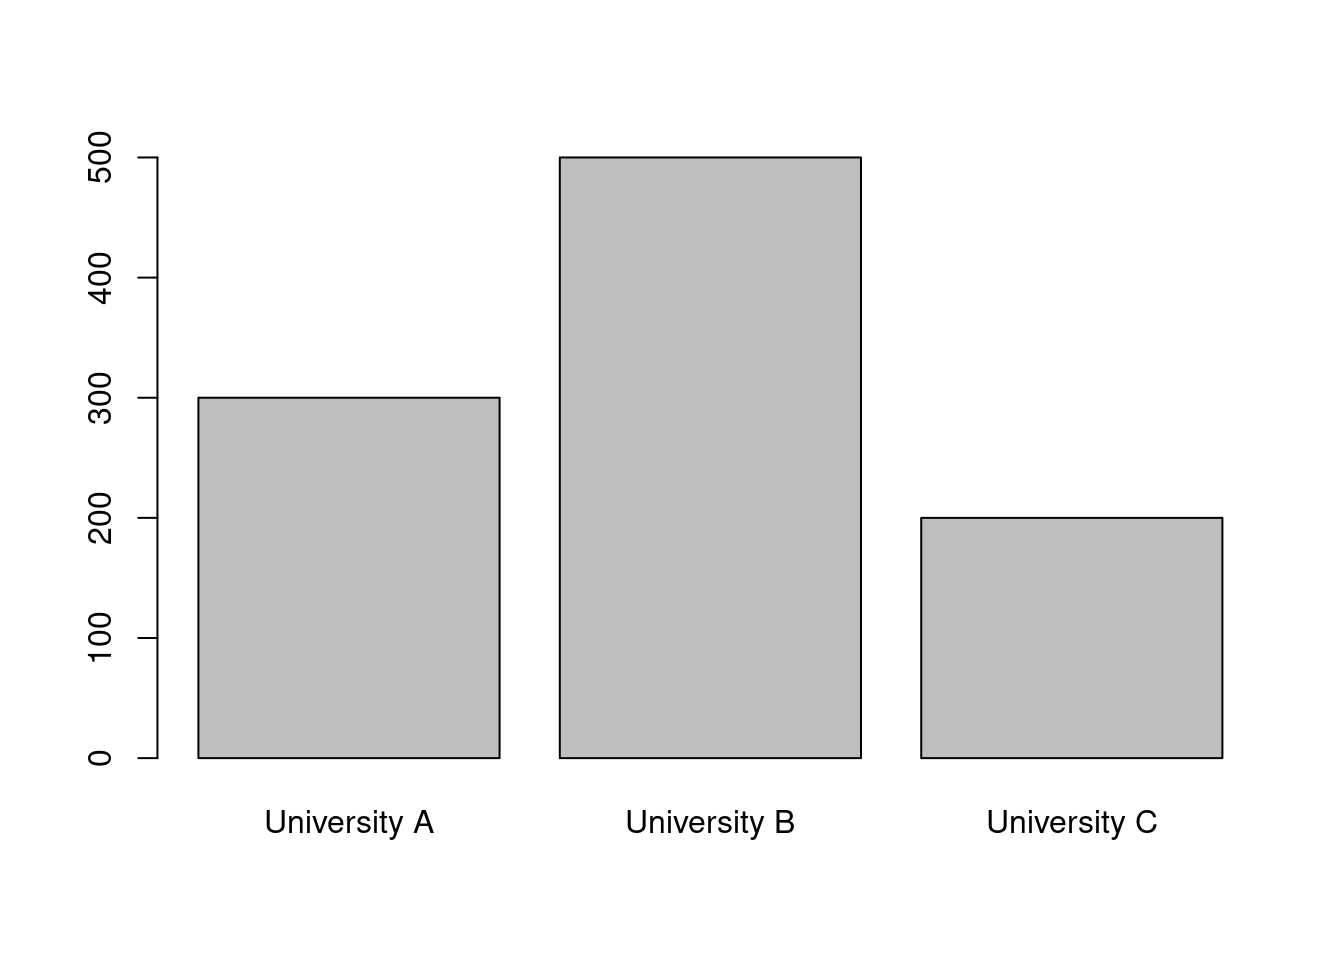
\includegraphics{_main_files/figure-latex/unnamed-chunk-245-1.pdf}

\subsubsection{Plot a categorical and a continuous variable}\label{plot-a-categorical-and-a-continuous-variable}

\texttt{plot()} with a categorical variable \texttt{x} and a continuous variable \texttt{y} shows a box plot with the distribution of continuous data in the factor levels.

\begin{Shaded}
\begin{Highlighting}[]
\FunctionTok{plot}\NormalTok{(}\AttributeTok{x =}\NormalTok{ simulation}\SpecialCharTok{$}\NormalTok{school, }\AttributeTok{y =}\NormalTok{ simulation}\SpecialCharTok{$}\NormalTok{IQ\_A)}
\end{Highlighting}
\end{Shaded}

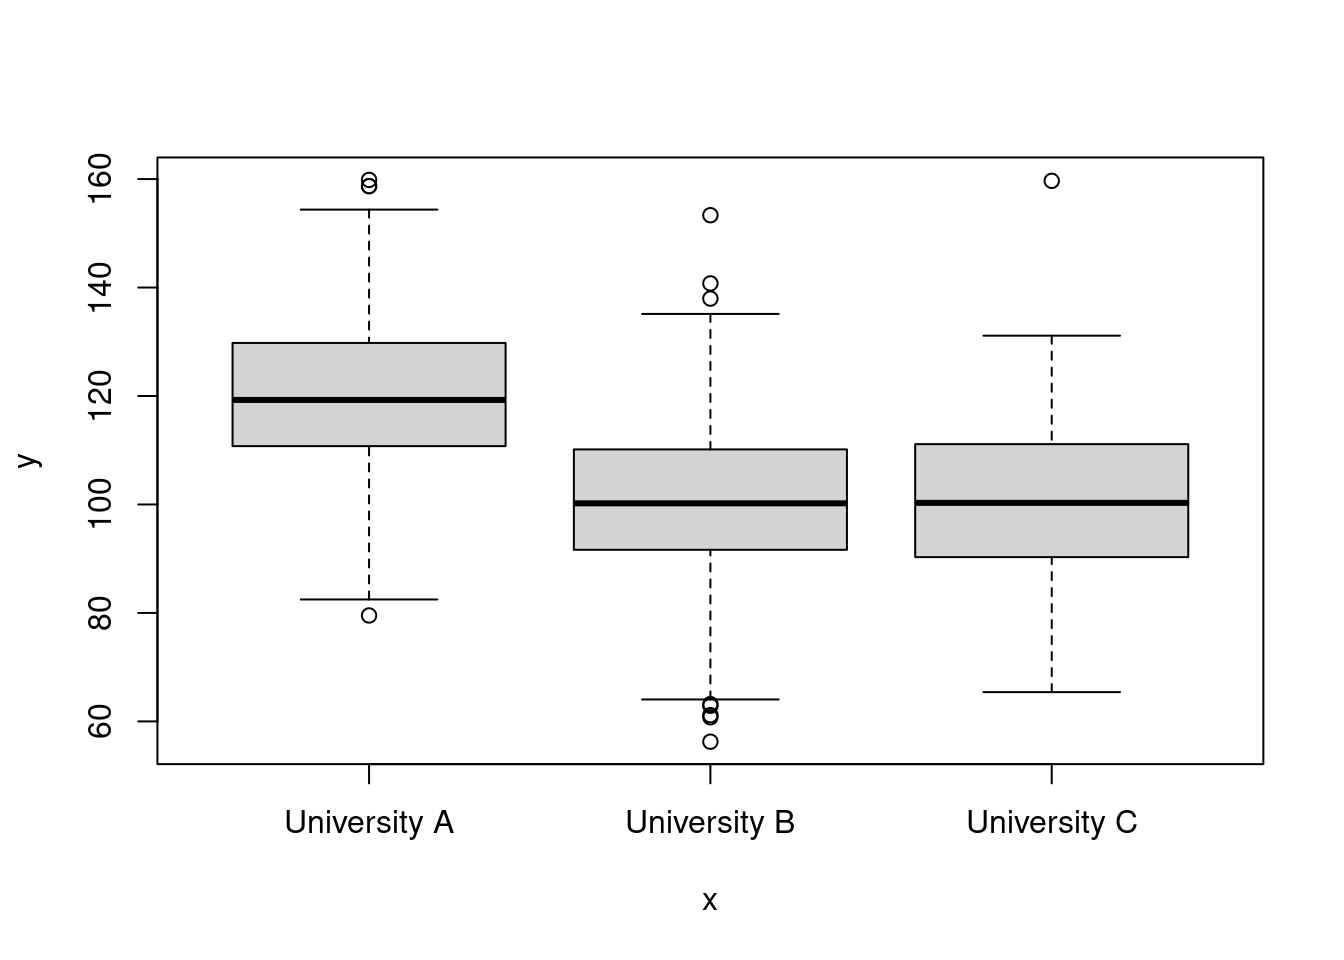
\includegraphics{_main_files/figure-latex/unnamed-chunk-246-1.pdf}

\subsubsection{Plot two continuous variables}\label{plot-two-continuous-variables}

\texttt{plot()} with a categorical variable \texttt{x} and a continuous variable \texttt{y} shows a scatter plot of the two variables. You see that \texttt{IQ\_A} and \texttt{IQ\_B} are correlated.

\begin{Shaded}
\begin{Highlighting}[]
\FunctionTok{plot}\NormalTok{(}\AttributeTok{x =}\NormalTok{ simulation}\SpecialCharTok{$}\NormalTok{IQ\_A, }\AttributeTok{y =}\NormalTok{ simulation}\SpecialCharTok{$}\NormalTok{IQ\_B)}
\end{Highlighting}
\end{Shaded}

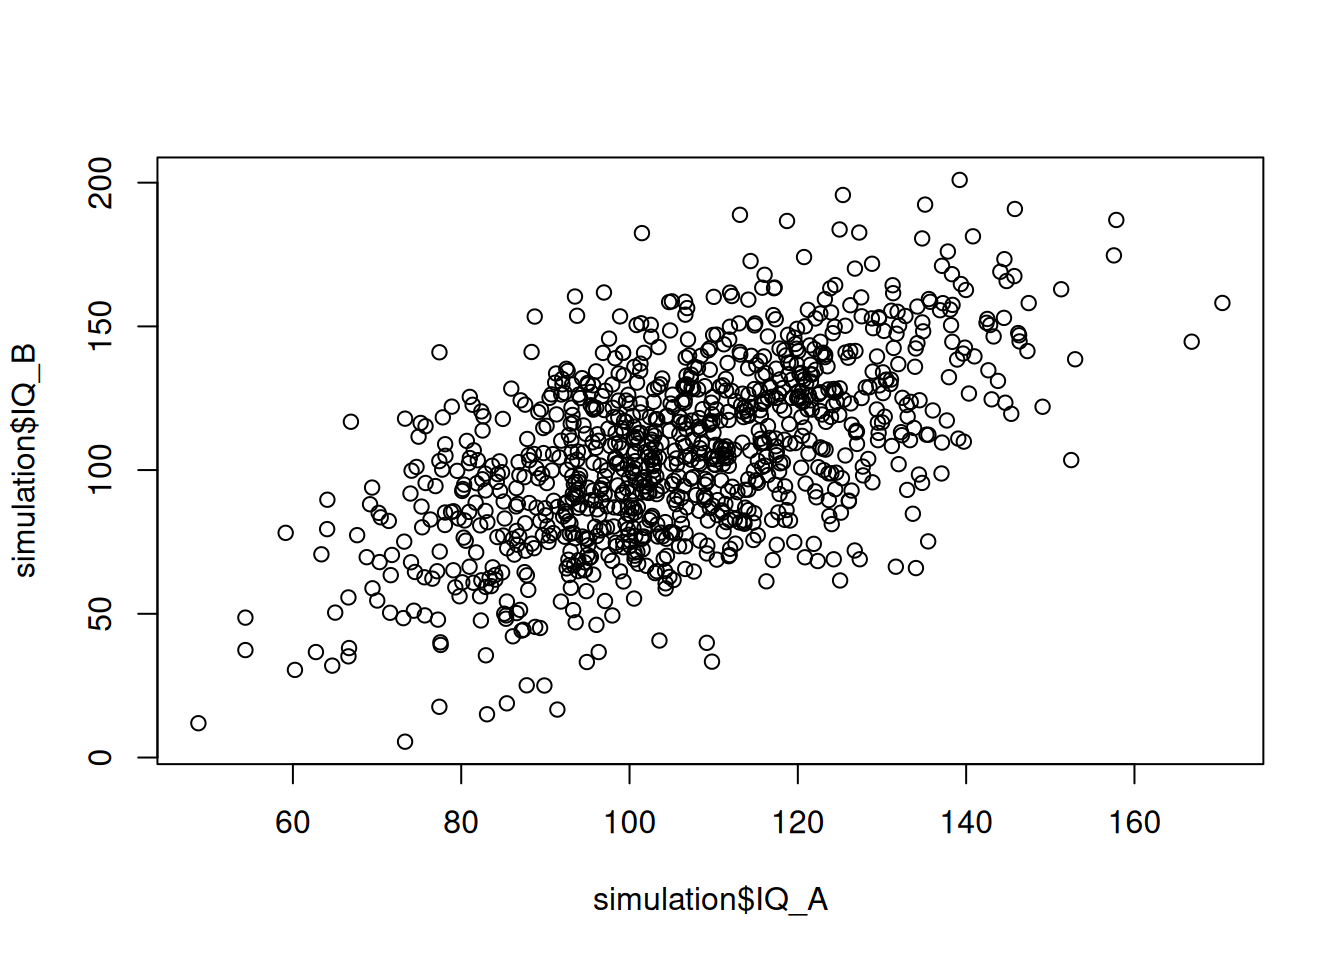
\includegraphics{_main_files/figure-latex/unnamed-chunk-247-1.pdf}
\webexhide{Excursus: Correlation coefficient}

By the way: To calculate the correlation coefficient \(r\), you can use the function \texttt{cor()}.

\begin{Shaded}
\begin{Highlighting}[]
\FunctionTok{cor}\NormalTok{(simulation}\SpecialCharTok{$}\NormalTok{IQ\_A, simulation}\SpecialCharTok{$}\NormalTok{IQ\_B)}
\end{Highlighting}
\end{Shaded}

\begin{verbatim}
## [1] 0.5437347
\end{verbatim}

\webexunhide

\subsection{ggplot2: Plotting in Tidyverse}\label{ggplot2-plotting-in-tidyverse}

While the functions above are nice for quick visualisations, it's difficult to make publication-ready plots. The package \texttt{ggplot2}, which is also part of the \emph{Tidyverse} ), is one of the most common packages to visualise data in \emph{R}.

\texttt{ggplot2} creates plots using a ``grammar of graphics'' where you add \texttt{geoms} in layers. It can be complex to understand, but it's very powerful once you have a mental model of how it works. The chapter will just illustrate the principle. Please have a look at the suggested literature above, if you want to know more.

Let's start with a totally empty plot layer created by the\texttt{ggplot()} function with no arguments.

\begin{Shaded}
\begin{Highlighting}[]
\FunctionTok{ggplot}\NormalTok{()}
\end{Highlighting}
\end{Shaded}


\includegraphics{_main_files/figure-latex/unnamed-chunk-249-1.pdf}

Like with all \emph{Tidyverse} functions, the first argument to \texttt{ggplot()} is the data frame you want to plot. We use our simulated data \texttt{simulation}.

\textbf{Aesthetic mappings}: The second argument is the mapping that specifies which variables corresponds to which properties of the plot, such as the \texttt{x}-axis, the \texttt{y}-axis, line \texttt{colour} or \texttt{linetype}, point \texttt{shape}, or object \texttt{fill}. These mappings are called the \emph{aesthetics} and are defined in \emph{R} by the \texttt{aes()} function. Just adding this to the \texttt{ggplot()} function creates the labels and ranges for the \texttt{x} and \texttt{y} axes. They usually have sensible default values, given your data, but you can also change them.

\begin{Shaded}
\begin{Highlighting}[]
\FunctionTok{ggplot}\NormalTok{(simulation, }\AttributeTok{mapping =} \FunctionTok{aes}\NormalTok{(}\AttributeTok{x=}\NormalTok{IQ\_A, }\AttributeTok{y=}\NormalTok{IQ\_B))}
\end{Highlighting}
\end{Shaded}

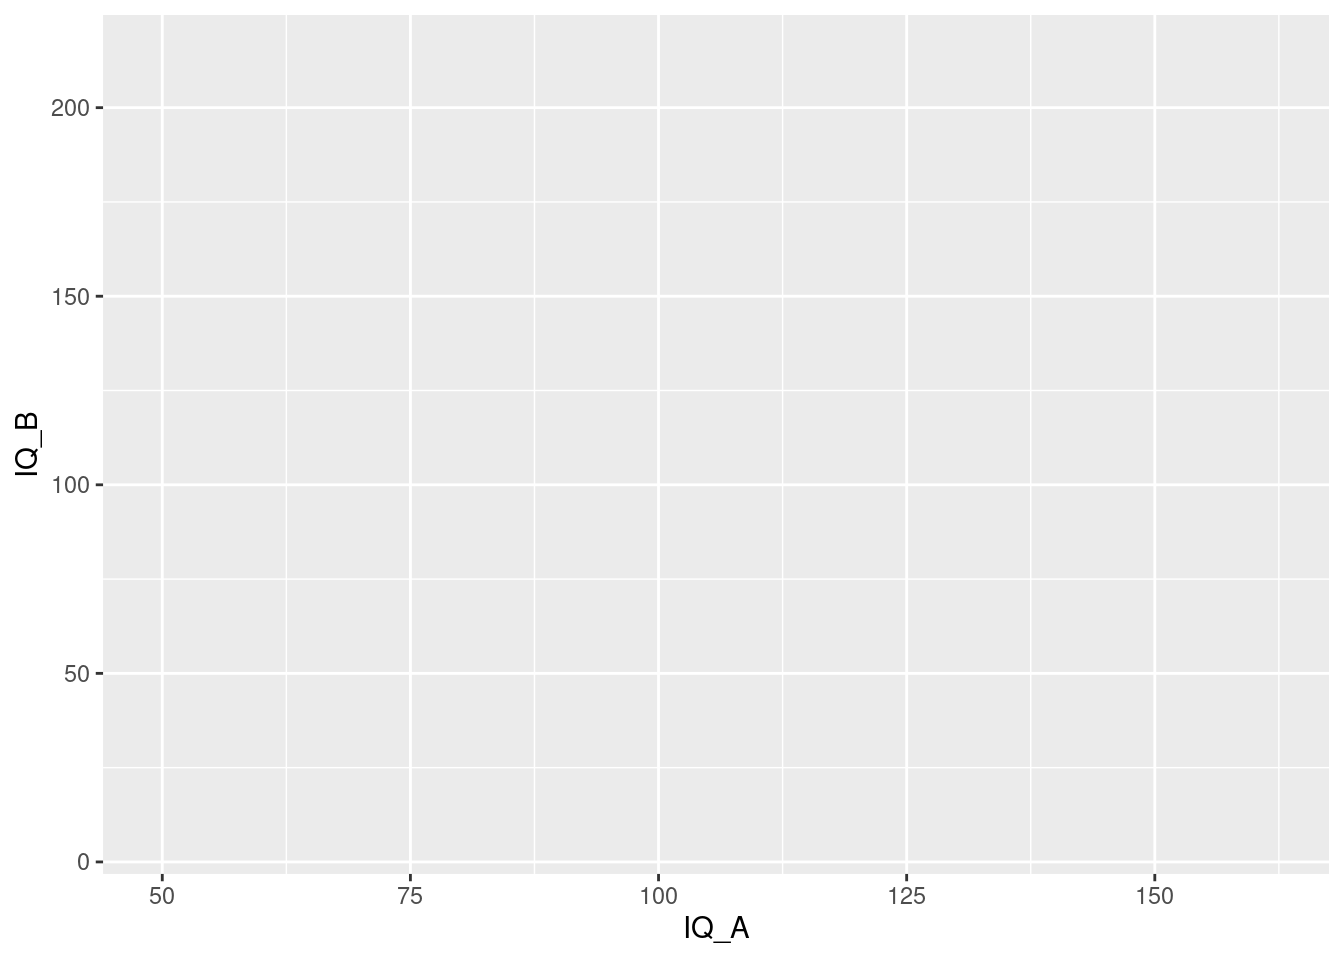
\includegraphics{_main_files/figure-latex/unnamed-chunk-250-1.pdf}

People often omit the argument name \texttt{mapping} and just put the \texttt{aes()} function directly as the second argument to \texttt{ggplot}. That's also fine. You can also omit \texttt{x} and \texttt{y} as arguments inside \texttt{aes()}, but I suggest to use argument names if you more than one variable, because it improves the readability.

The function above does not plot anything yet and you only see scaled axes with the variable names. \emph{R} does not yet know \emph{what} or better \emph{how} to plot the data. This will be specified in \texttt{ggplot2} by ``geoms'' or plot styles. You literally add them with the \texttt{+} symbol. You can also add other plot attributes, such as labels, or change the theme and the font size (see the advanced literature).

If we add, for example, the \texttt{geom\_point()}, we tell \emph{R} to plot the data with the defined aesthetic mapping as point:

\begin{Shaded}
\begin{Highlighting}[]
\FunctionTok{ggplot}\NormalTok{(simulation, }\AttributeTok{mapping =} \FunctionTok{aes}\NormalTok{(}\AttributeTok{x=}\NormalTok{IQ\_A, }\AttributeTok{y=}\NormalTok{IQ\_B)) }\SpecialCharTok{+} \FunctionTok{geom\_point}\NormalTok{()}
\end{Highlighting}
\end{Shaded}

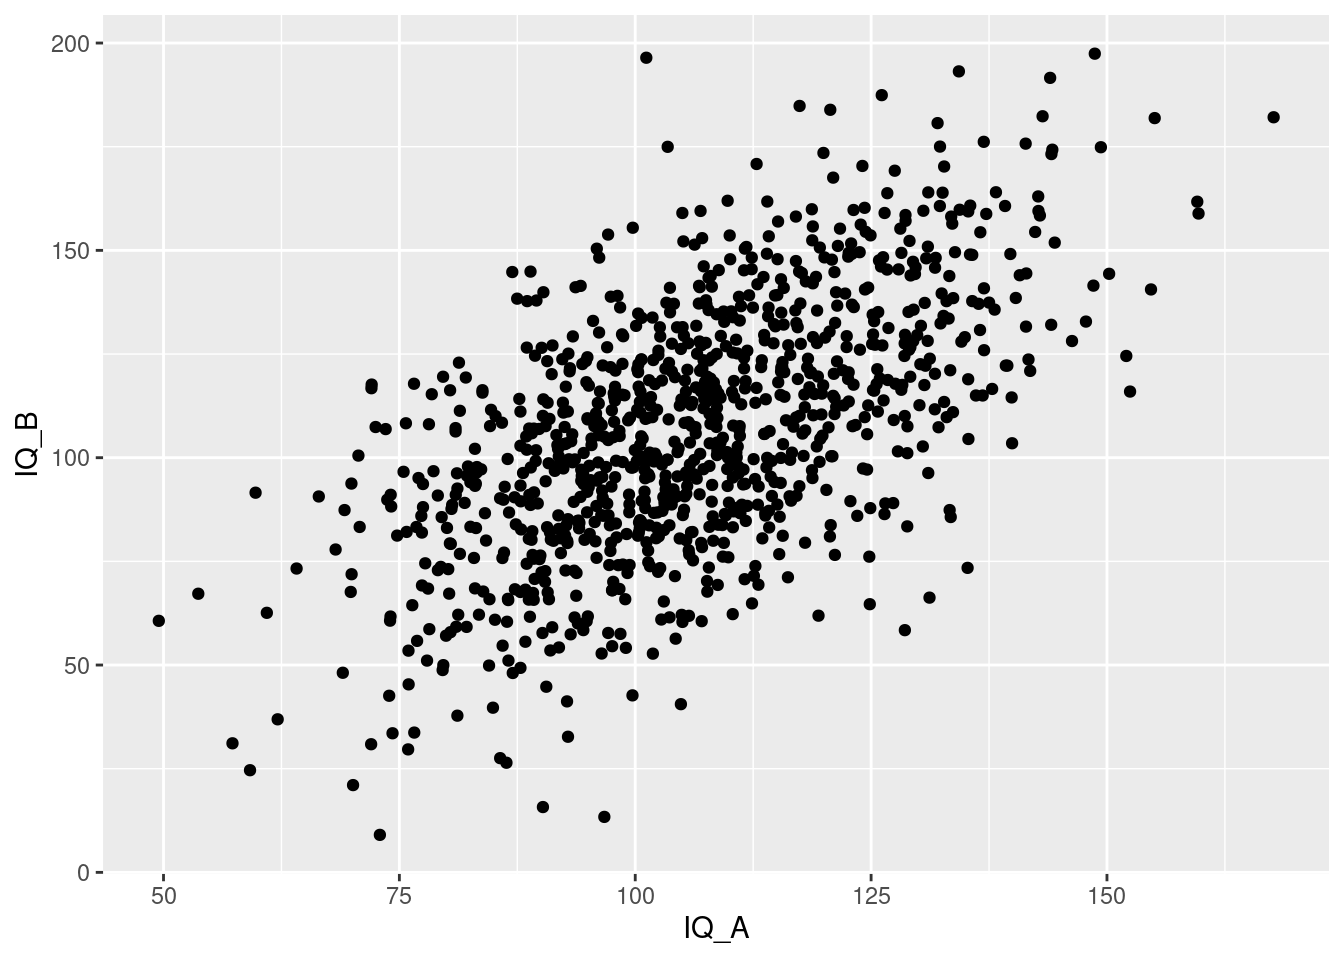
\includegraphics{_main_files/figure-latex/unnamed-chunk-251-1.pdf}

\subsection{Geoms or plot types}\label{geoms-or-plot-types}

There are many geoms, and they can take different arguments to customise their appearance. Lets have a look a common plot types. Look carefully at the code to see the different mappings, \texttt{aes()}, and geoms, \texttt{geom\_?()}. This ways you get hopefully a bit of an inside how the functions work. As you know, if you want information about these functions, you can always look at the function documentation by typing \texttt{?function\_name}.

\subsubsection{Bar plot}\label{bar-plot}

Bar plot are done pity easy by adding (\texttt{+}) the geom \texttt{geom\_bar()}:

\begin{Shaded}
\begin{Highlighting}[]
\FunctionTok{ggplot}\NormalTok{(simulation, }\FunctionTok{aes}\NormalTok{(school)) }\SpecialCharTok{+}
        \FunctionTok{geom\_bar}\NormalTok{()}
\end{Highlighting}
\end{Shaded}

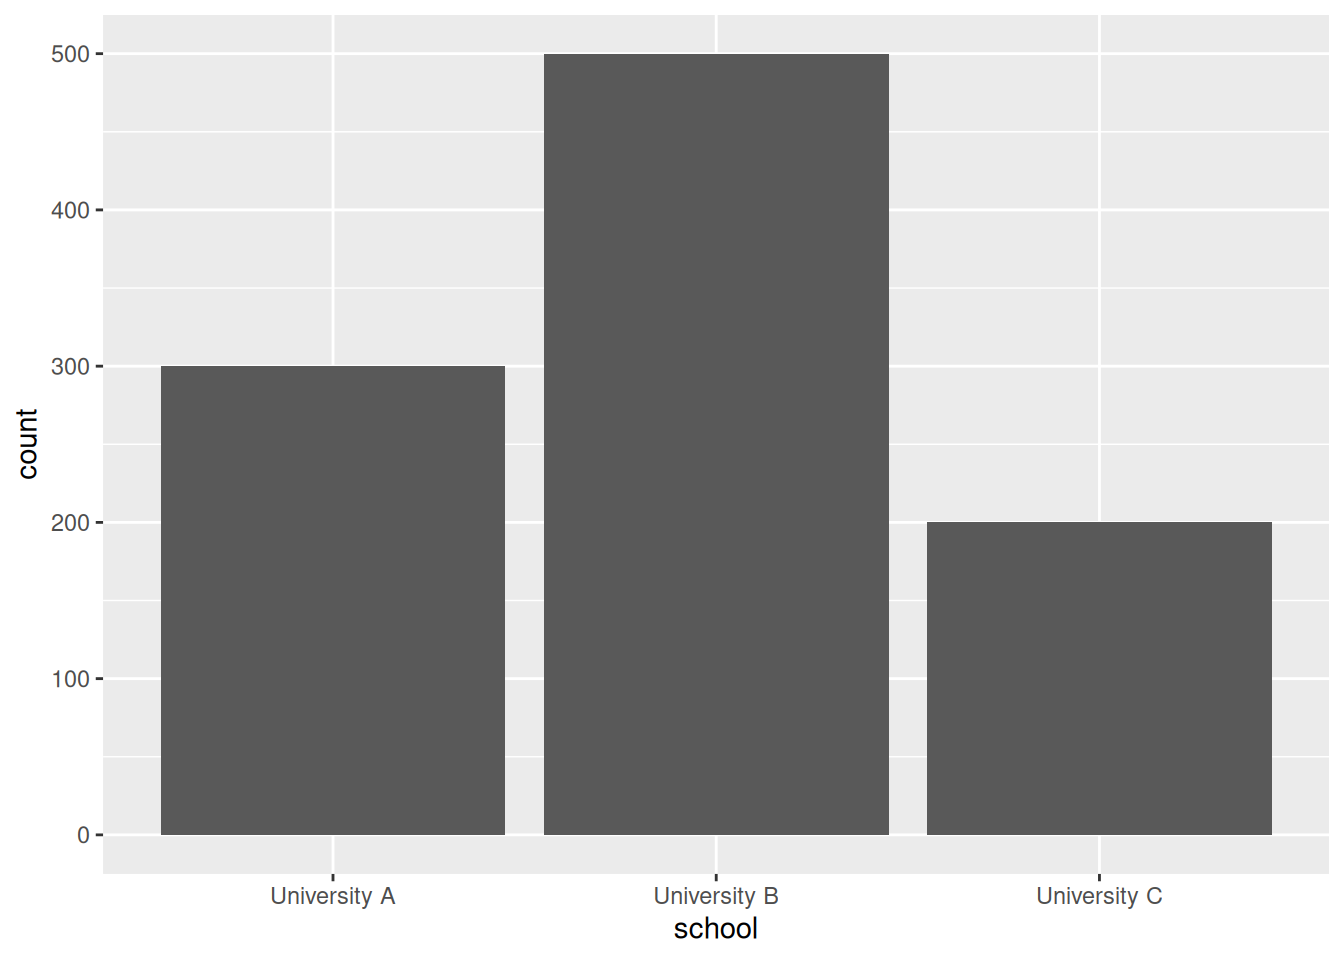
\includegraphics{_main_files/figure-latex/unnamed-chunk-252-1.pdf}

\subsubsection{Density plots}\label{density-plots}

Density plots are good for one continuous variable, but only if you have a fairly large number of observations.

\begin{Shaded}
\begin{Highlighting}[]
\FunctionTok{ggplot}\NormalTok{(simulation, }\FunctionTok{aes}\NormalTok{(IQ\_A)) }\SpecialCharTok{+}
        \FunctionTok{geom\_density}\NormalTok{()}
\end{Highlighting}
\end{Shaded}

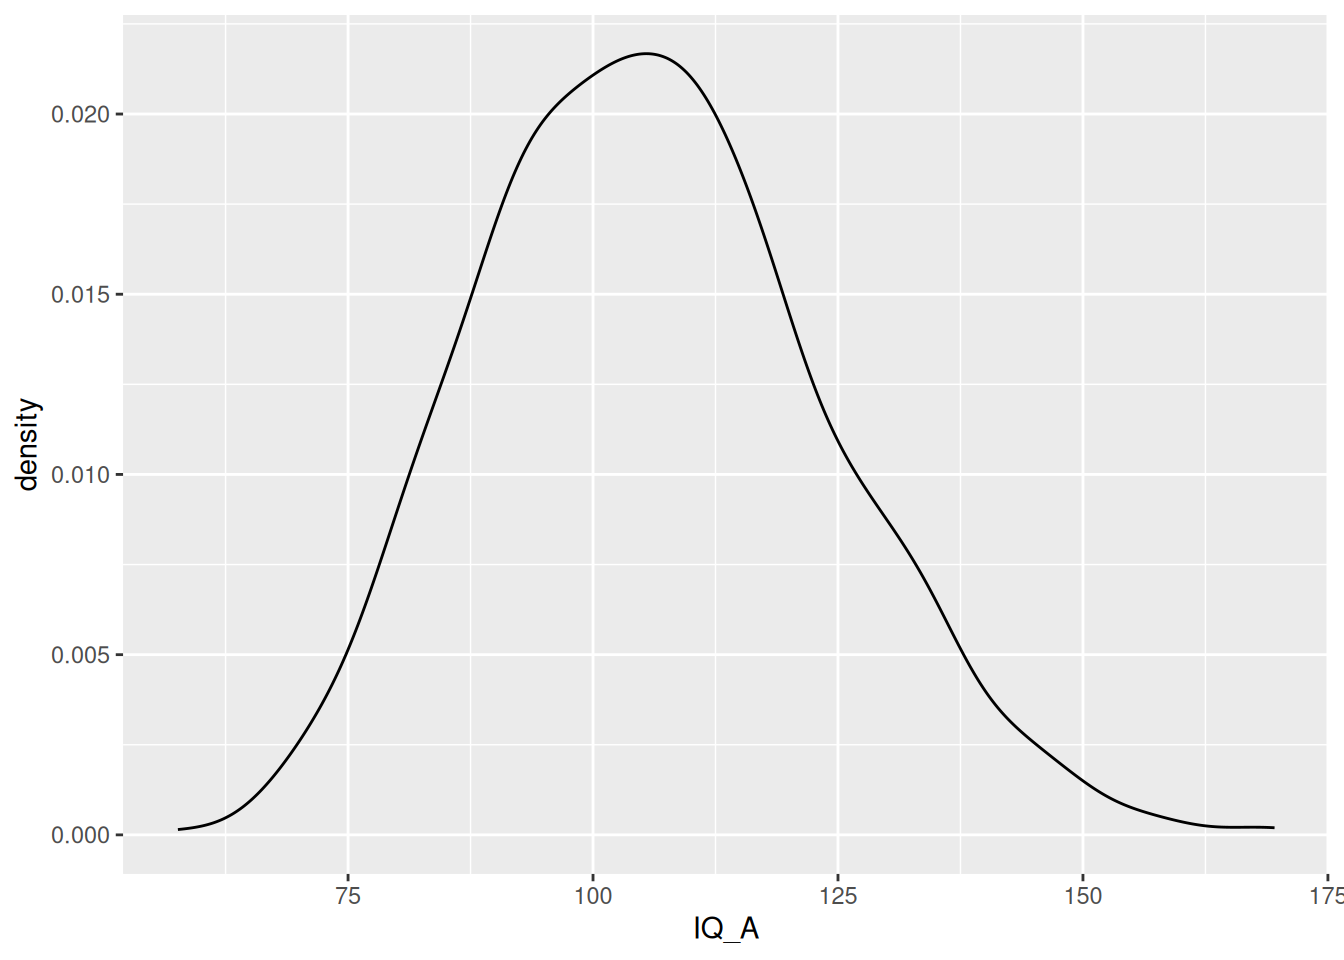
\includegraphics{_main_files/figure-latex/unnamed-chunk-253-1.pdf}

You can represent subsets of a variable by assigning the category variable to the argument \texttt{group}, \texttt{fill}, or \texttt{color}.

\begin{Shaded}
\begin{Highlighting}[]
\FunctionTok{ggplot}\NormalTok{(simulation, }\FunctionTok{aes}\NormalTok{(IQ\_A, }\AttributeTok{color=}\NormalTok{school)) }\SpecialCharTok{+}
        \FunctionTok{geom\_density}\NormalTok{(}\AttributeTok{alpha=}\FloatTok{0.7}\NormalTok{)}
\end{Highlighting}
\end{Shaded}

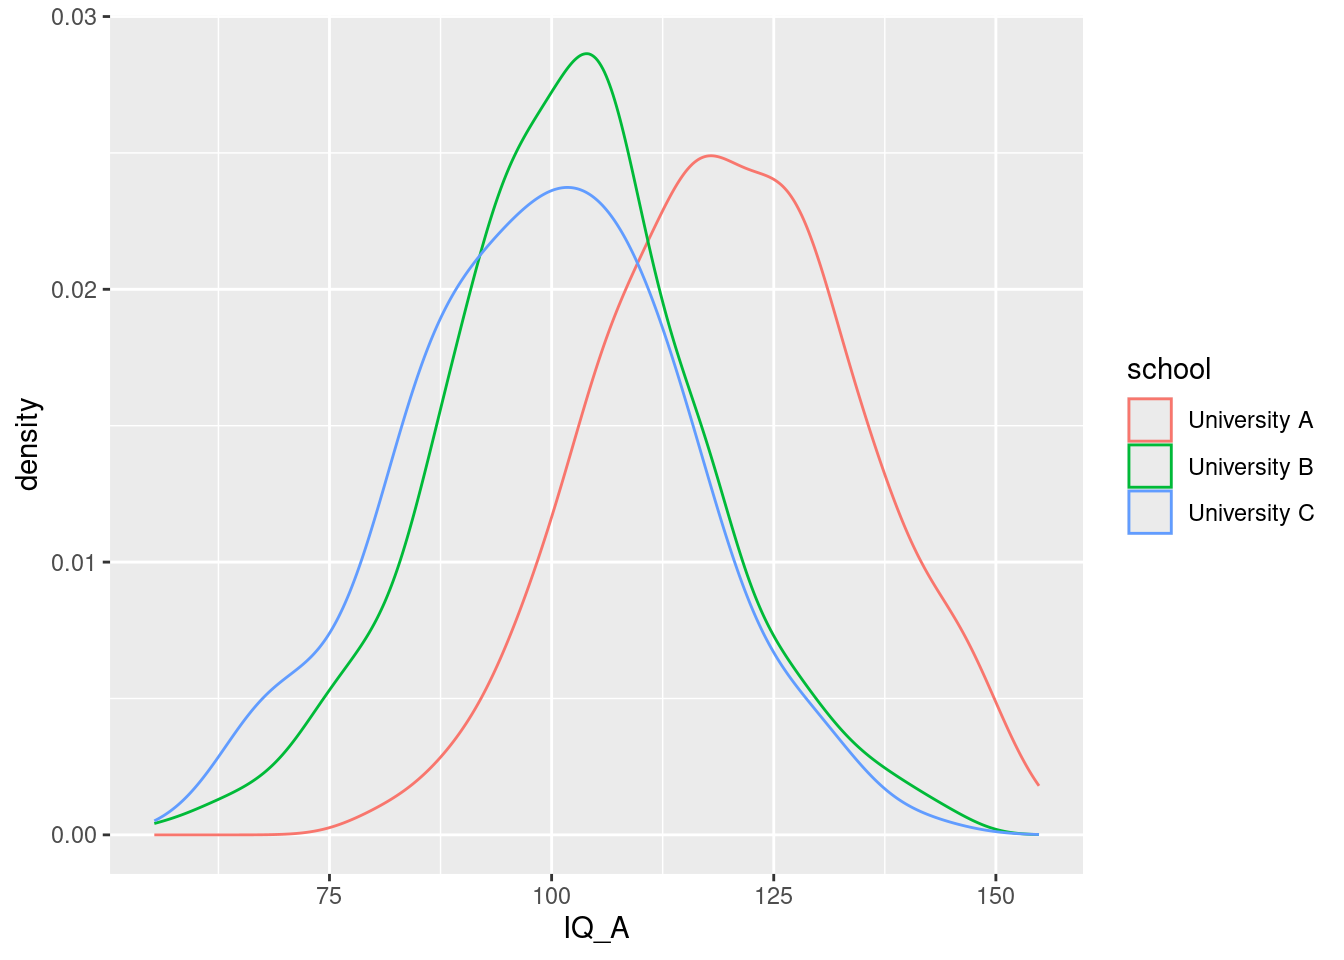
\includegraphics{_main_files/figure-latex/unnamed-chunk-254-1.pdf}

\begin{Shaded}
\begin{Highlighting}[]
\FunctionTok{ggplot}\NormalTok{(simulation, }\FunctionTok{aes}\NormalTok{(IQ\_A, }\AttributeTok{fill=}\NormalTok{school)) }\SpecialCharTok{+}
        \FunctionTok{geom\_density}\NormalTok{(}\AttributeTok{alpha=}\FloatTok{0.7}\NormalTok{)}
\end{Highlighting}
\end{Shaded}

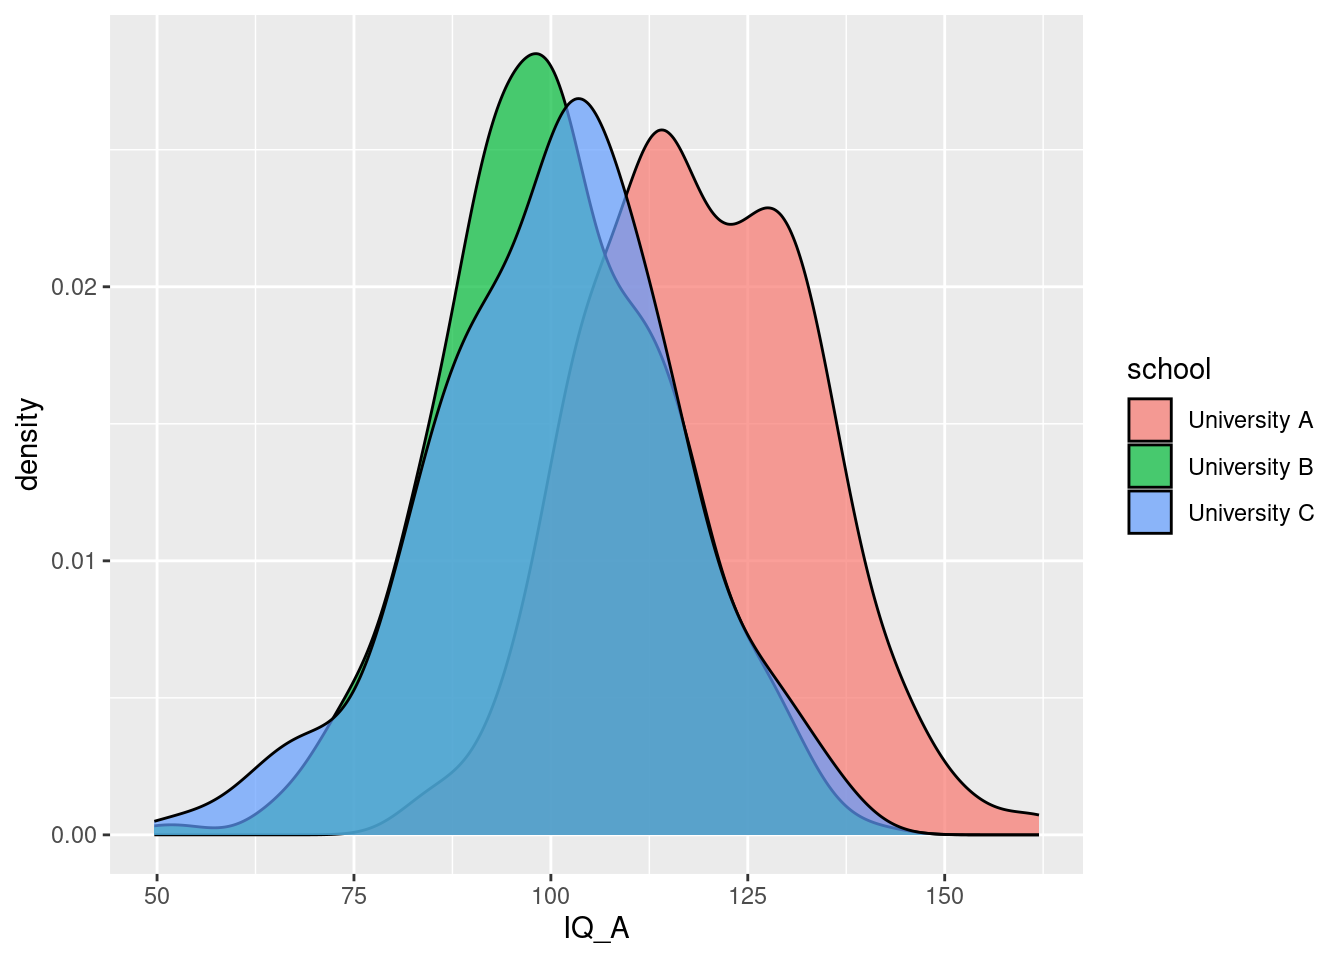
\includegraphics{_main_files/figure-latex/unnamed-chunk-255-1.pdf}

\subsubsection{Histogram}\label{histogram}

Histogram are useful to get an overview on the shape of the distribution of your continuous data.

\begin{Shaded}
\begin{Highlighting}[]
\FunctionTok{ggplot}\NormalTok{(simulation, }\FunctionTok{aes}\NormalTok{(IQ\_A)) }\SpecialCharTok{+}
        \FunctionTok{geom\_histogram}\NormalTok{()}
\end{Highlighting}
\end{Shaded}

\begin{verbatim}
## `stat_bin()` using `bins = 30`. Pick better value with `binwidth`.
\end{verbatim}

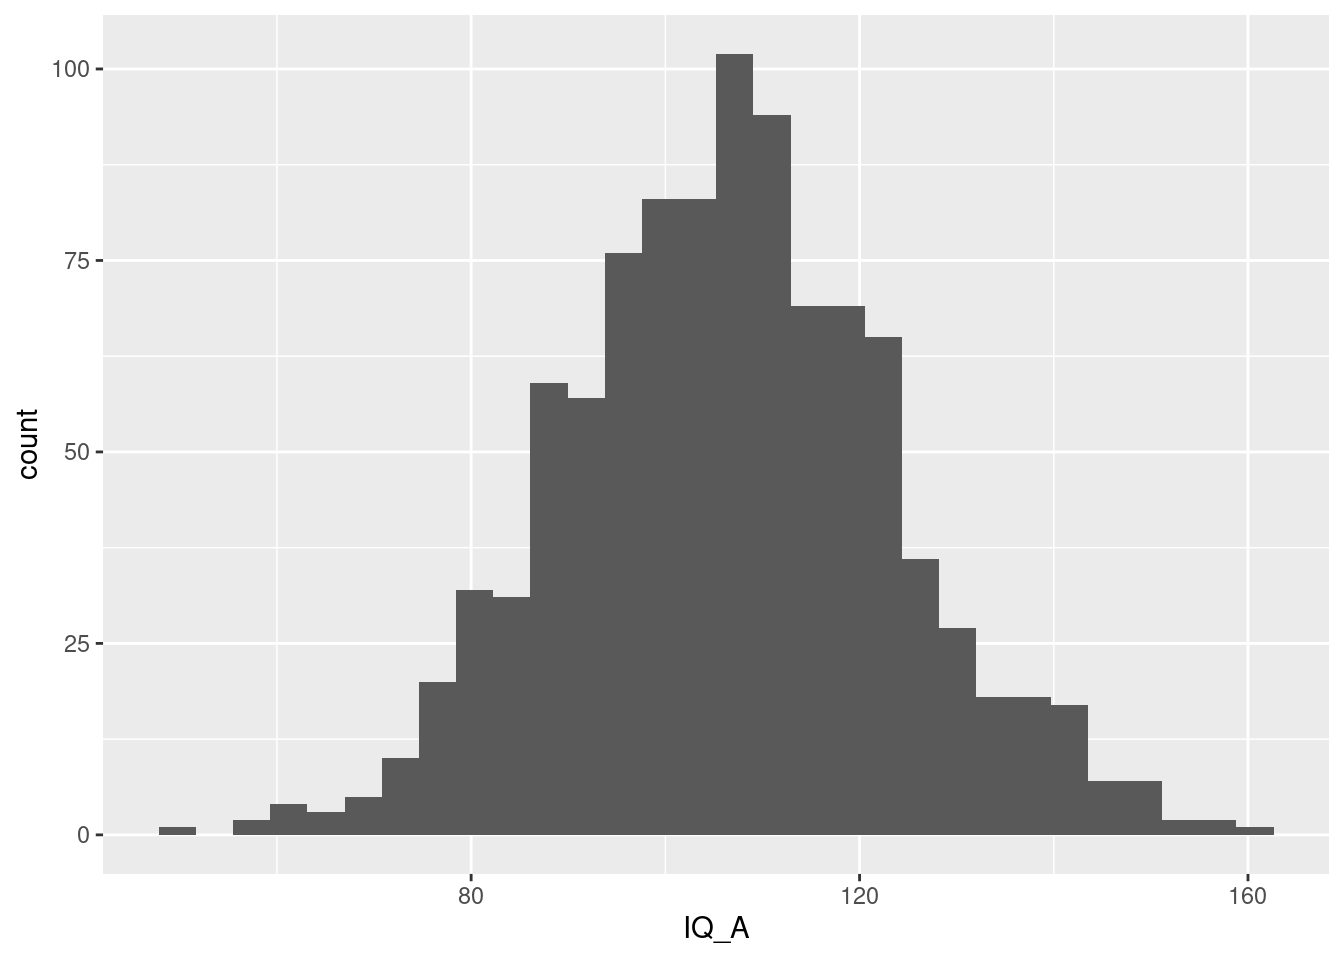
\includegraphics{_main_files/figure-latex/unnamed-chunk-256-1.pdf}

If you don't like the colours, don't panic:

\begin{Shaded}
\begin{Highlighting}[]
\FunctionTok{ggplot}\NormalTok{(simulation, }\FunctionTok{aes}\NormalTok{(IQ\_A)) }\SpecialCharTok{+}
    \FunctionTok{geom\_histogram}\NormalTok{(}\AttributeTok{binwidth =} \DecValTok{5}\NormalTok{, }\AttributeTok{fill =} \StringTok{"white"}\NormalTok{, }\AttributeTok{color =} \StringTok{"black"}\NormalTok{)}
\end{Highlighting}
\end{Shaded}

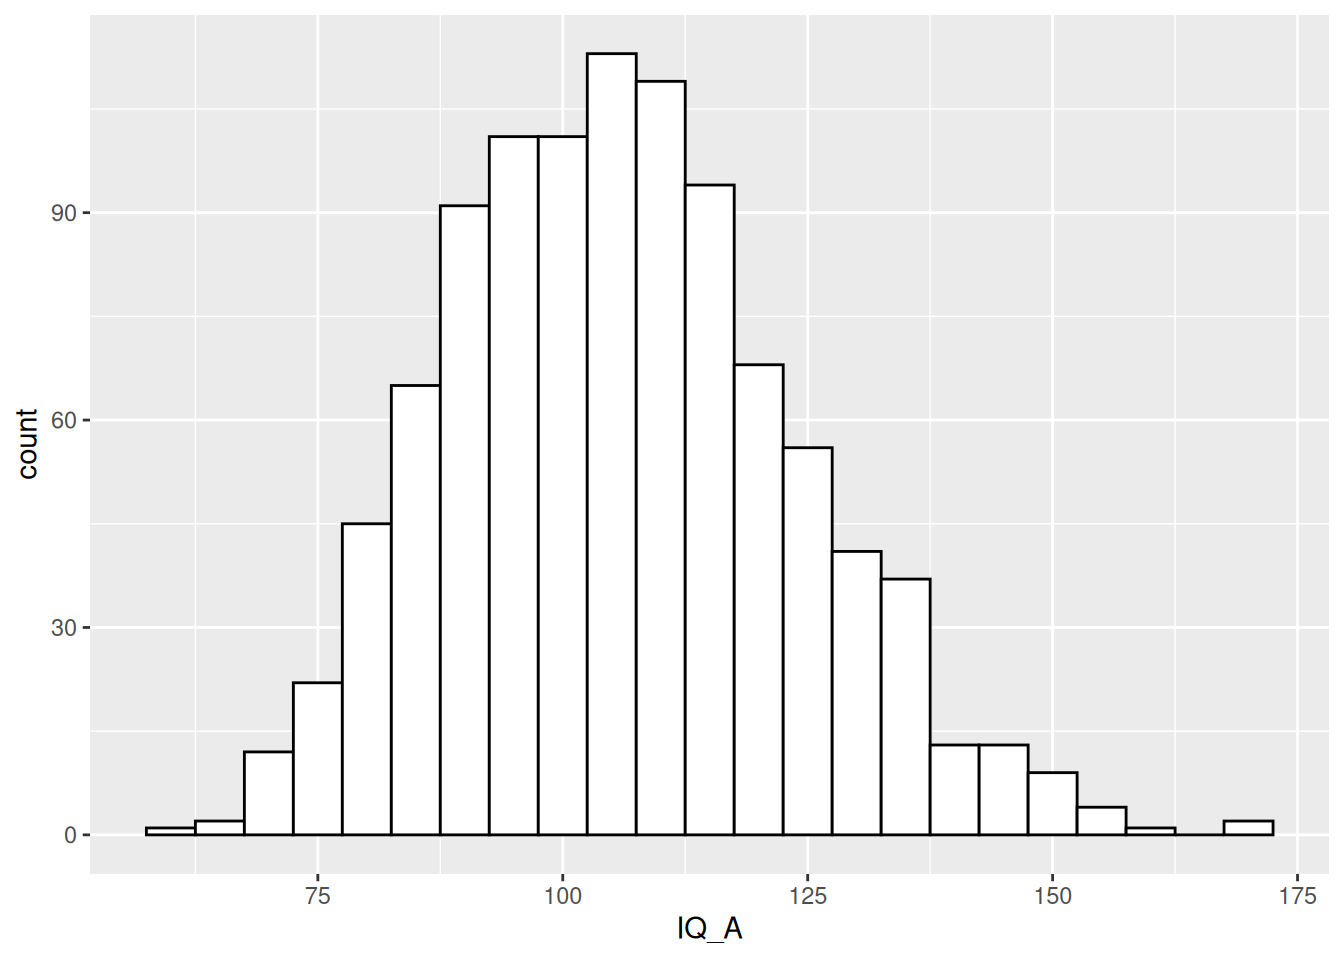
\includegraphics{_main_files/figure-latex/unnamed-chunk-257-1.pdf}

Again, you can add the factor variable the mapping (\texttt{aes()}) of the plot and make different histograms for each factor level.

\begin{Shaded}
\begin{Highlighting}[]
\FunctionTok{ggplot}\NormalTok{(simulation, }\FunctionTok{aes}\NormalTok{(IQ\_A, }\AttributeTok{fill =}\NormalTok{ school)) }\SpecialCharTok{+}
      \FunctionTok{geom\_histogram}\NormalTok{(}\AttributeTok{alpha =} \FloatTok{0.5}\NormalTok{)}
\end{Highlighting}
\end{Shaded}

\begin{verbatim}
## `stat_bin()` using `bins = 30`. Pick better value with `binwidth`.
\end{verbatim}

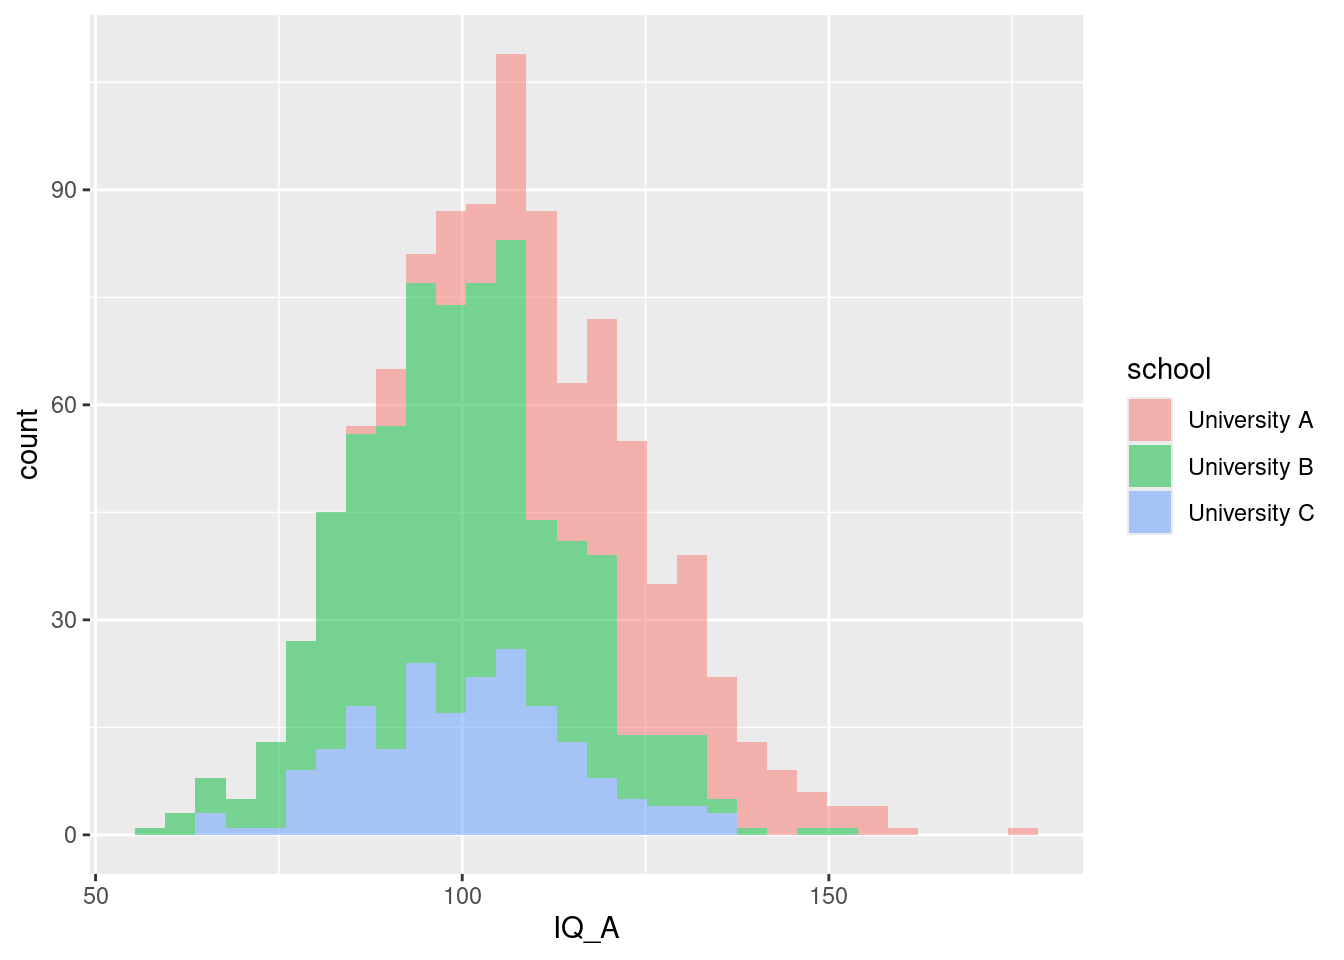
\includegraphics{_main_files/figure-latex/unnamed-chunk-258-1.pdf}

\subsubsection{Column plots}\label{column-plots}

Column plots are the most common way to depict grouped continuous data. If your data are already aggregated with \texttt{summarise()} (see chapter \ref{summarising}), you can use \texttt{geom\_bar} (and \texttt{geom\_col} and \texttt{geom\_errorbar}) to make this plots.

If not, you can use the function \texttt{stat\_summary} to calculate the mean and standard error and send those numbers to the appropriate geom for plotting.

\begin{Shaded}
\begin{Highlighting}[]
\FunctionTok{ggplot}\NormalTok{(simulation, }\FunctionTok{aes}\NormalTok{(}\AttributeTok{x=}\NormalTok{school, }\AttributeTok{y=}\NormalTok{IQ\_A, }\AttributeTok{fill=}\NormalTok{school)) }\SpecialCharTok{+}
  \FunctionTok{stat\_summary}\NormalTok{(}\AttributeTok{fun =}\NormalTok{ mean, }\AttributeTok{geom =} \StringTok{"col"}\NormalTok{, }\AttributeTok{alpha =} \FloatTok{0.5}\NormalTok{) }\SpecialCharTok{+}
  \FunctionTok{stat\_summary}\NormalTok{(}\AttributeTok{fun.data =}\NormalTok{ mean\_se, }\AttributeTok{geom =} \StringTok{"errorbar"}\NormalTok{, }\AttributeTok{width =} \FloatTok{0.25}\NormalTok{) }\SpecialCharTok{+}
  \FunctionTok{coord\_cartesian}\NormalTok{(}\AttributeTok{ylim =} \FunctionTok{c}\NormalTok{(}\DecValTok{80}\NormalTok{, }\DecValTok{120}\NormalTok{))}
\end{Highlighting}
\end{Shaded}

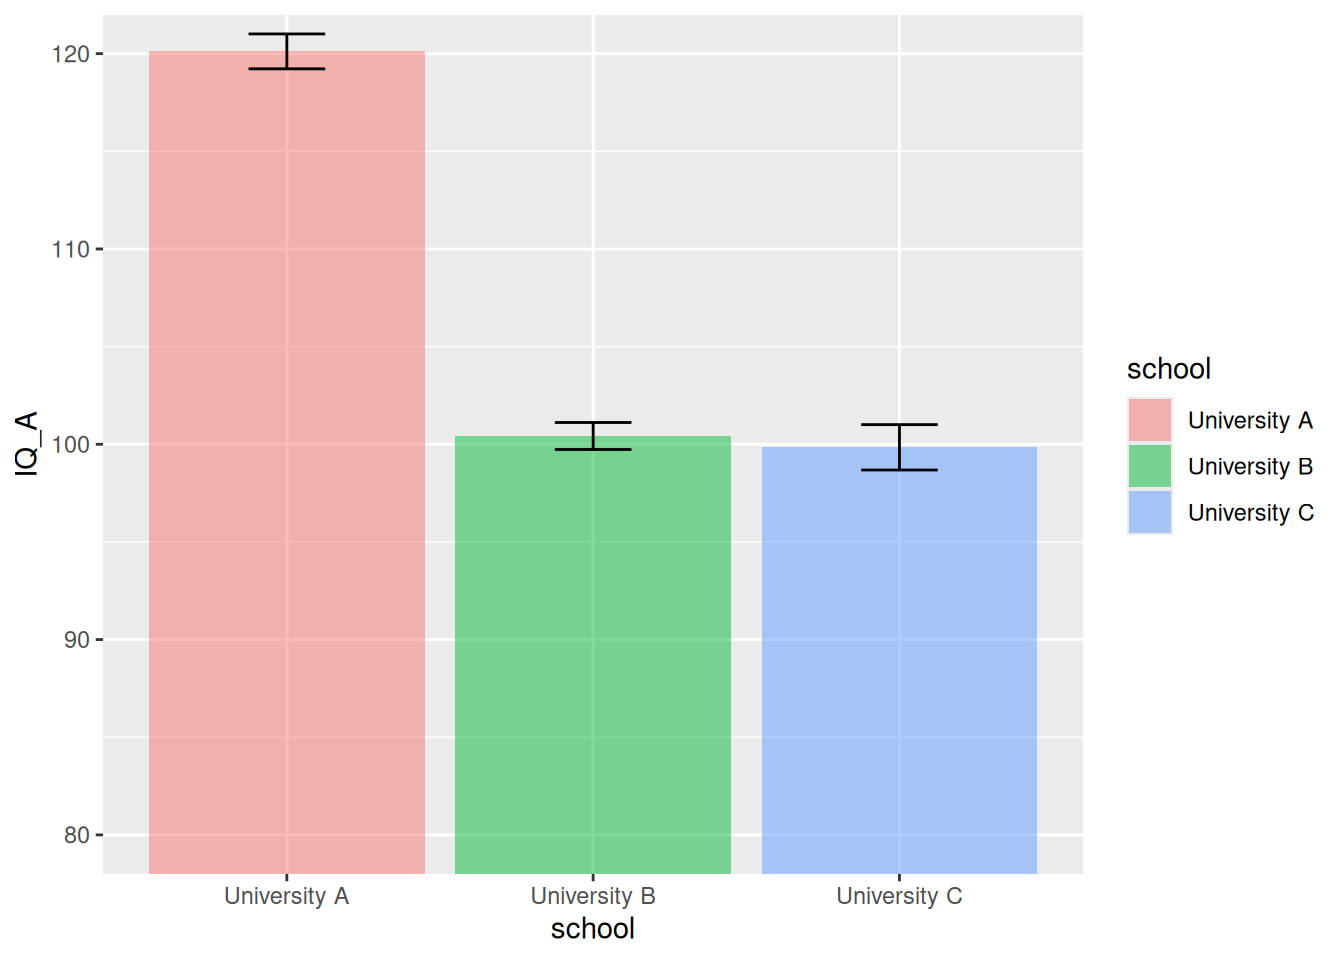
\includegraphics{_main_files/figure-latex/unnamed-chunk-259-1.pdf}

\subsubsection{Box plots}\label{box-plots}

Boxplots are, I my view, a much better way to depict grouped continuous data, because they provide some information about the distribution and about outliers. Unfortunately, they are less common in psychology and social sciences. With \texttt{ggplot2}, it's very easy to do:

\begin{Shaded}
\begin{Highlighting}[]
\FunctionTok{ggplot}\NormalTok{(simulation, }\FunctionTok{aes}\NormalTok{(}\AttributeTok{x=}\NormalTok{school, }\AttributeTok{y=}\NormalTok{IQ\_A, }\AttributeTok{fill=}\NormalTok{school)) }\SpecialCharTok{+}
  \FunctionTok{geom\_boxplot}\NormalTok{(}\AttributeTok{alpha =} \FloatTok{0.5}\NormalTok{)}
\end{Highlighting}
\end{Shaded}

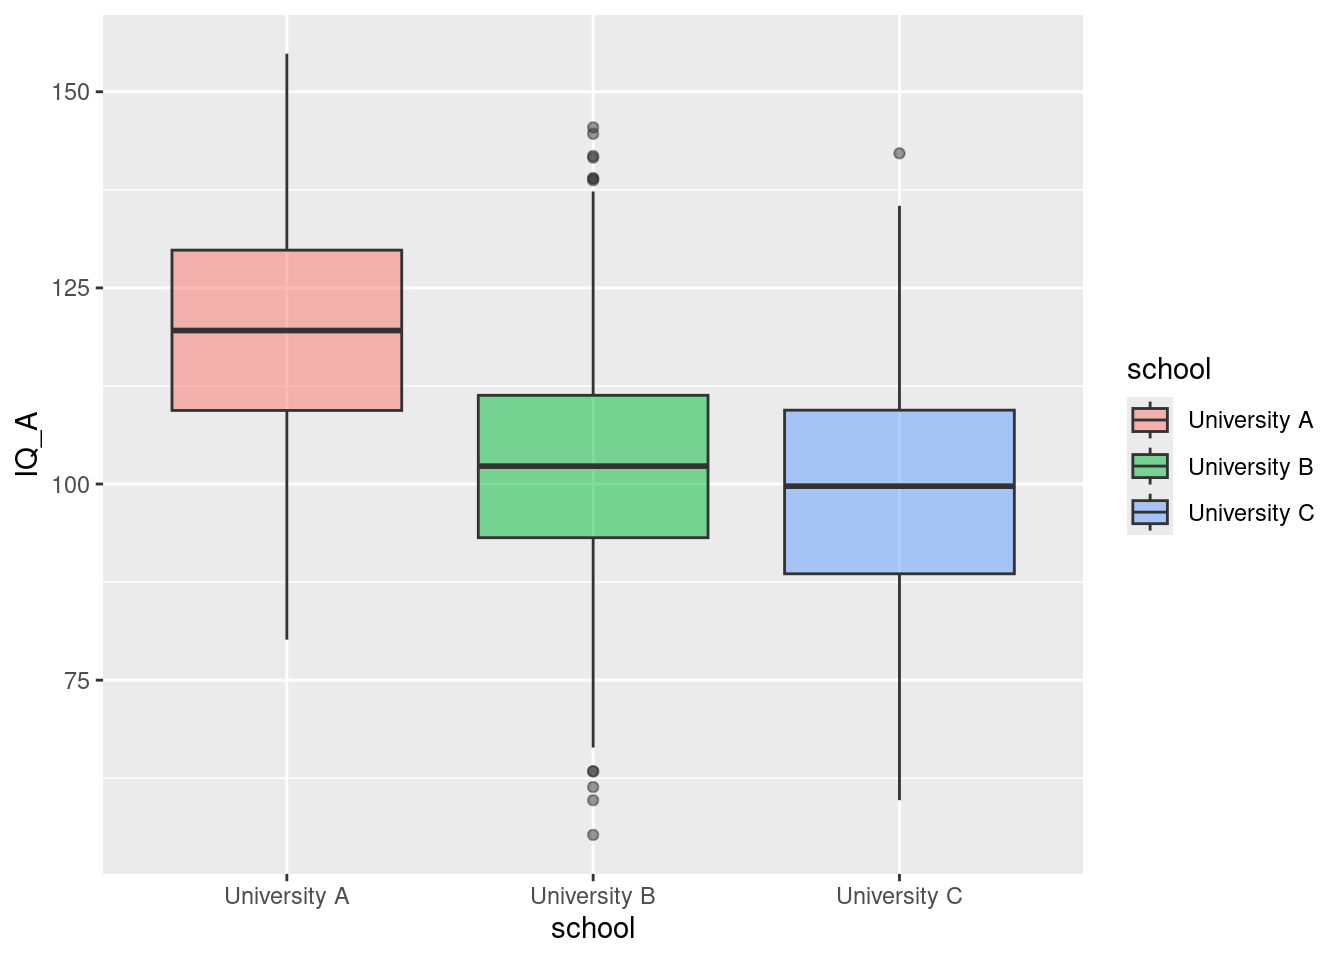
\includegraphics{_main_files/figure-latex/unnamed-chunk-260-1.pdf}

\subsubsection{Violin pots}\label{violin-pots}

Violin pots are like sideways, mirrored density plots. They give even more direct information about distribution and are, in my view, useful when you have non-normal distributions.

\begin{Shaded}
\begin{Highlighting}[]
\FunctionTok{ggplot}\NormalTok{(simulation, }\FunctionTok{aes}\NormalTok{(}\AttributeTok{x=}\NormalTok{school, }\AttributeTok{y=}\NormalTok{IQ\_A, }\AttributeTok{fill=}\NormalTok{school)) }\SpecialCharTok{+}
    \FunctionTok{geom\_violin}\NormalTok{(}\AttributeTok{draw\_quantiles =}\NormalTok{ .}\DecValTok{5}\NormalTok{, }\AttributeTok{trim =} \ConstantTok{FALSE}\NormalTok{, }\AttributeTok{alpha =} \FloatTok{0.5}\NormalTok{)}
\end{Highlighting}
\end{Shaded}

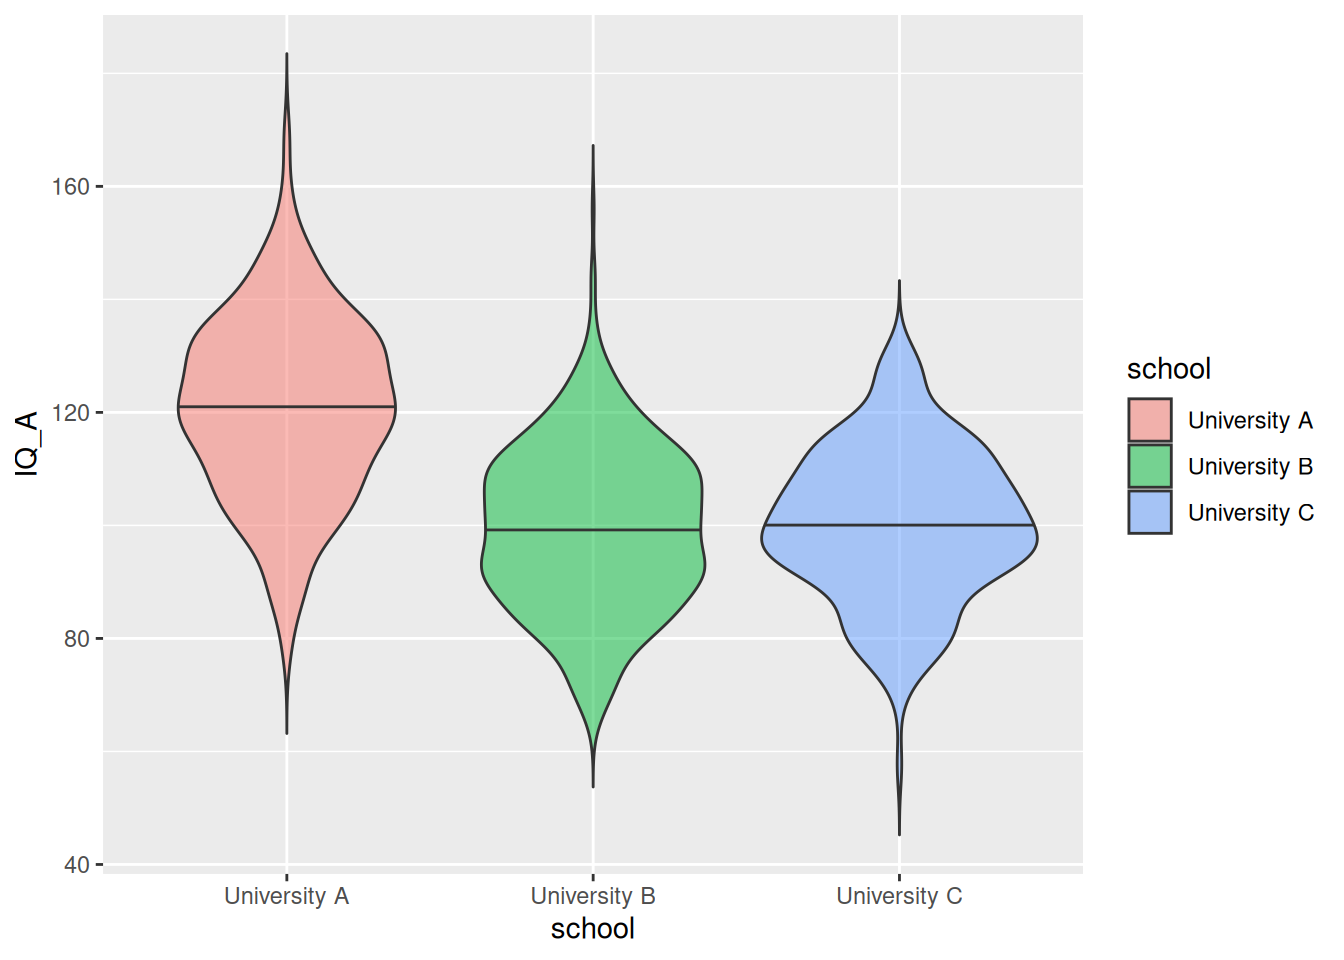
\includegraphics{_main_files/figure-latex/unnamed-chunk-261-1.pdf}

\subsubsection{Scatter plot}\label{scatter-plot}

Let's plot \texttt{IQ\_A} on the \texttt{x} and \texttt{IQ\_B} on the \texttt{y}-axes and take also the \texttt{school} into account:

\begin{Shaded}
\begin{Highlighting}[]
\FunctionTok{ggplot}\NormalTok{(simulation, }\FunctionTok{aes}\NormalTok{(IQ\_A, IQ\_B, }\AttributeTok{color=}\NormalTok{school)) }\SpecialCharTok{+}
  \FunctionTok{geom\_point}\NormalTok{(}\AttributeTok{alpha =} \FloatTok{0.7}\NormalTok{) }\SpecialCharTok{+}
  \FunctionTok{theme\_classic}\NormalTok{()}
\end{Highlighting}
\end{Shaded}

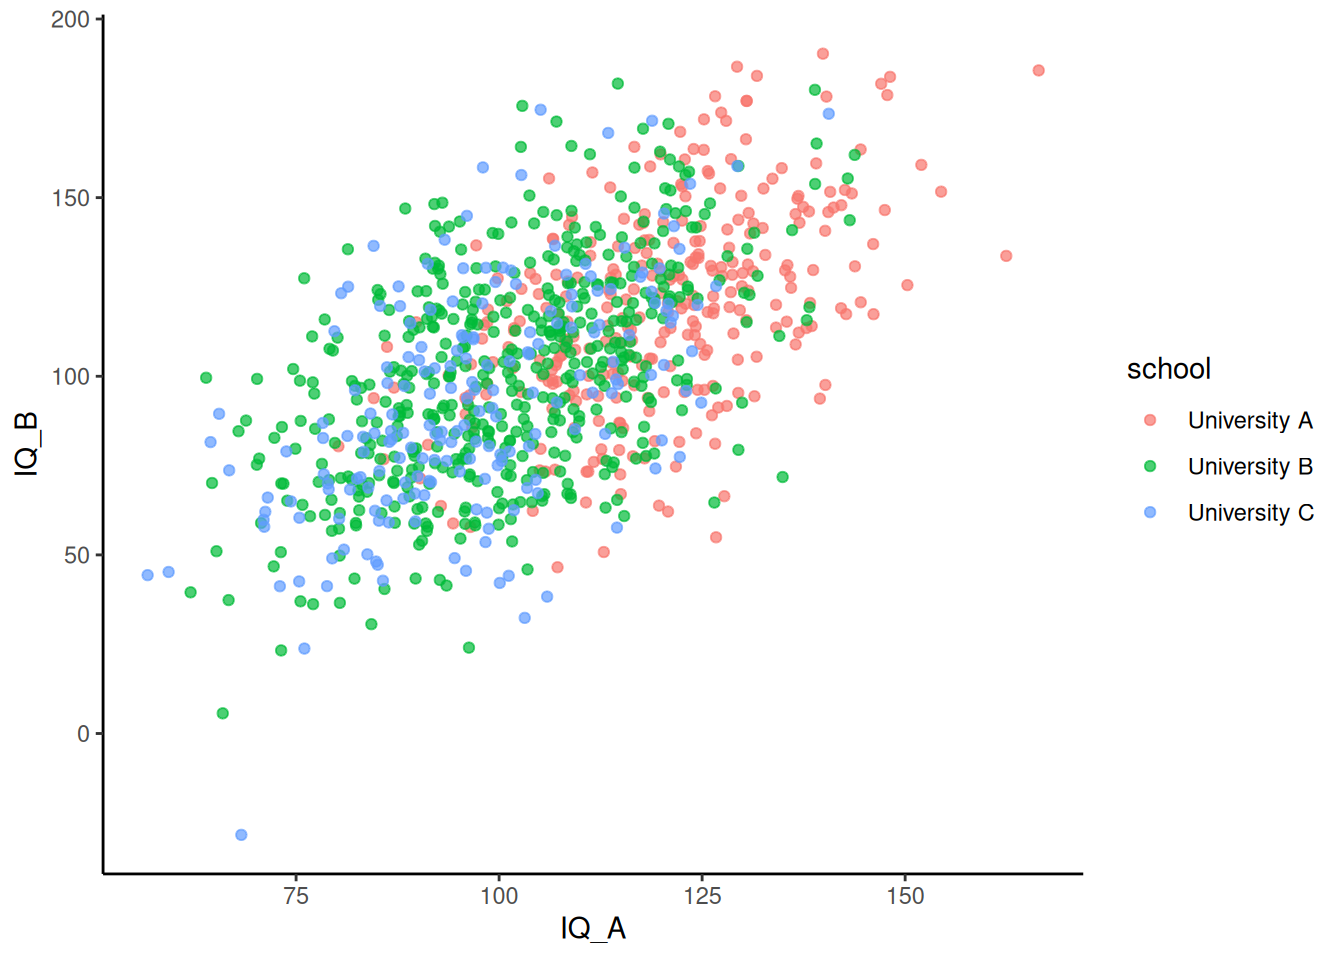
\includegraphics{_main_files/figure-latex/unnamed-chunk-262-1.pdf}

\subsubsection{Line graph}\label{line-graph}

To illustrate the correlation between the two variables, we can plot line graph that depicts the regression line.

\begin{Shaded}
\begin{Highlighting}[]
\FunctionTok{ggplot}\NormalTok{(simulation, }\FunctionTok{aes}\NormalTok{(IQ\_A, IQ\_B)) }\SpecialCharTok{+}
  \FunctionTok{geom\_smooth}\NormalTok{(}\AttributeTok{formula =}\NormalTok{ y }\SpecialCharTok{\textasciitilde{}}\NormalTok{ x, }\AttributeTok{method=}\StringTok{"lm"}\NormalTok{)}
\end{Highlighting}
\end{Shaded}

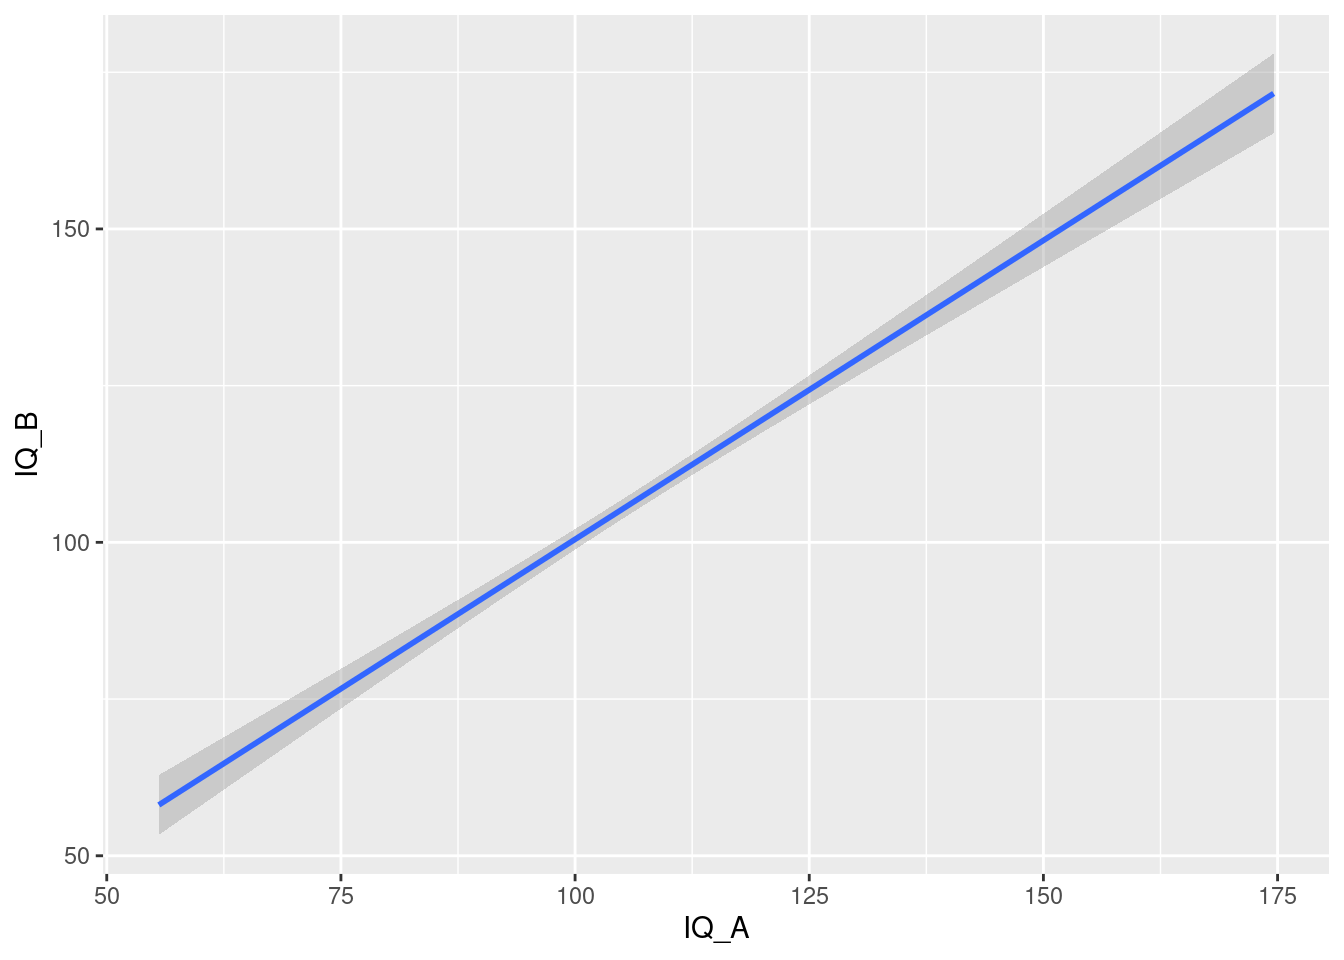
\includegraphics{_main_files/figure-latex/unnamed-chunk-263-1.pdf}

\subsubsection{Combining two plot types}\label{combining-two-plot-types}

Finally, it's also possible the combine two plot types, such a line and scatter plot:

\begin{Shaded}
\begin{Highlighting}[]
\FunctionTok{ggplot}\NormalTok{(simulation, }\FunctionTok{aes}\NormalTok{(IQ\_A, IQ\_B)) }\SpecialCharTok{+}
  \FunctionTok{geom\_point}\NormalTok{(}\AttributeTok{alpha =} \FloatTok{0.7}\NormalTok{) }\SpecialCharTok{+}
  \FunctionTok{geom\_smooth}\NormalTok{(}\AttributeTok{formula =}\NormalTok{ y }\SpecialCharTok{\textasciitilde{}}\NormalTok{ x, }\AttributeTok{method=}\StringTok{"lm"}\NormalTok{) }\SpecialCharTok{+}
  \FunctionTok{theme\_classic}\NormalTok{()}
\end{Highlighting}
\end{Shaded}

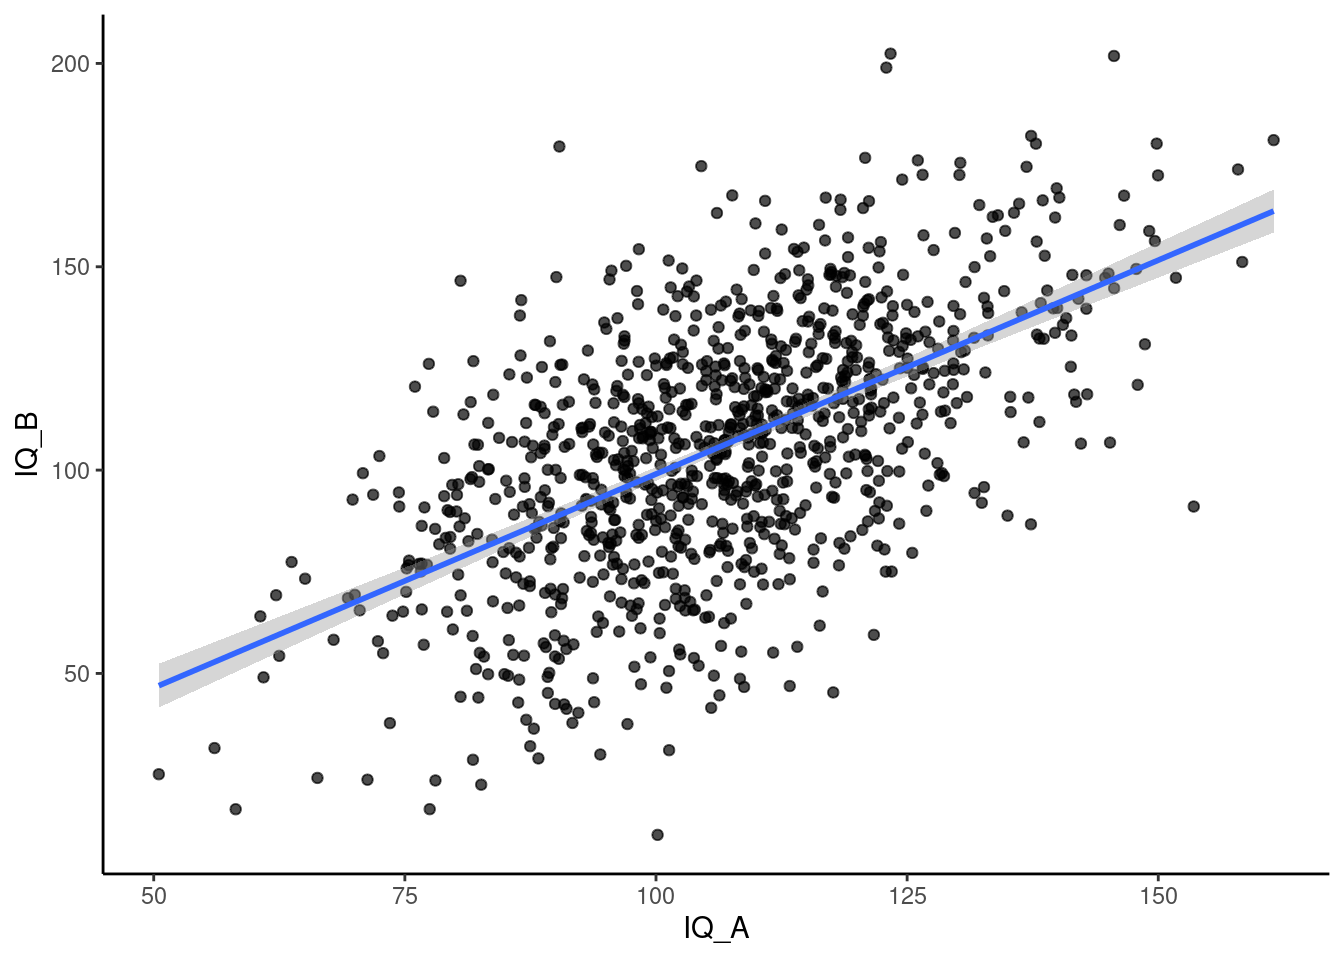
\includegraphics{_main_files/figure-latex/unnamed-chunk-264-1.pdf}

\newpage

\appendix


\section{Suggested Readings}\label{readings}

The following free books and online resources provide further introductions to data science skills with \emph{R}.

\begin{itemize}
\tightlist
\item
  \href{https://r4ds.had.co.nz/}{R for Data Science} by Grolemund \& Wickham
\item
  \href{https://rstudio-education.github.io/hopr/}{Hands-On Programming with R} by G. Grolemund
\item
  \href{https://adv-r.hadley.nz/}{Advanced R} by Hadley Wickham
\item
  \href{https://rstudio-education.github.io/tidyverse-cookbook}{The Tidyverse Cookbook} by G. Grolemund
\item
  \href{https://psyteachr.github.io/reprores-v3/index.html}{Data Skills for Reproducible Science} from the University Glasgow
\end{itemize}

Further resources

\begin{itemize}
\tightlist
\item
  \href{http://www.cookbook-r.com/}{R codebook}
\item
  \href{http://ohi-science.org/data-science-training/}{Introduction to Open Data Science}
\item
  \href{https://bookdown.org/rdpeng/exdata/}{Exploratory Data Analysis with R}
\item
  \href{https://bookdown.org/rdpeng/artofdatascience/}{The Art of Data Science}
\item
  \href{http://socviz.co/}{Data Visualization: A practical introduction}
\end{itemize}

\subsection{Cheat sheets}\label{cheatsheets}

\begin{itemize}
\tightlist
\item
  \href{https://raw.githubusercontent.com/rstudio/cheatsheets/main/rstudio-ide.pdf}{RStudio IDE}
\item
  \href{https://raw.githubusercontent.com/rstudio/cheatsheets/master/base-r.pdf}{Base R}
\item
  \href{https://raw.githubusercontent.com/rstudio/cheatsheets/main/data-import.pdf}{Data import} with \texttt{readr}
\item
  \href{https://raw.githubusercontent.com/rstudio/cheatsheets/main/data-transformation.pdf}{Data transformation} with \texttt{dplyr\ \&\ tidyr}
\item
  \href{https://raw.githubusercontent.com/rstudio/cheatsheets/master/tidyr.pdf}{Data tidying} with \texttt{tidyr}
\item
  \href{https://raw.githubusercontent.com/rstudio/cheatsheets/main/data-visualization.pdf}{Data visualization} with \texttt{ggplot}
\item
  \href{https://rstudio.com/resources/cheatsheets/}{and more..}
\end{itemize}

\section{Interesting Packages}\label{packagelist}

\begin{longtable}[]{@{}
  >{\raggedright\arraybackslash}p{(\columnwidth - 2\tabcolsep) * \real{0.5000}}
  >{\raggedright\arraybackslash}p{(\columnwidth - 2\tabcolsep) * \real{0.5000}}@{}}
\toprule\noalign{}
\begin{minipage}[b]{\linewidth}\raggedright
Name
\end{minipage} & \begin{minipage}[b]{\linewidth}\raggedright
Description
\end{minipage} \\
\midrule\noalign{}
\endhead
\bottomrule\noalign{}
\endlastfoot
\href{http://lubridate.tidyverse.org/}{lubridate} & Easy dealing with dates and times, see \href{https://r4ds.had.co.nz/dates-and-times.html}{tutorial} \\
\href{https://cran.r-project.org/web/packages/afex/}{afex} & Analysis of factorial experiments \\
\href{https://easystats.github.io/effectsize/}{effectsize} & Indices of effect size and standardized parameters \\
\href{https://cran.r-project.org/web/packages/pwr/}{pwr} & Basic functions for power analysis \\
\href{https://cran.r-project.org/web/packages/easypower}{easypower} & Sample size estimation for experimental designs \\
\href{https://www.lavaan.ugent.be/}{lavaan} & Factor analysis and structural equation modeling \\
\href{https://cran.r-project.org/web/packages/lme4/index.html}{lme4} & Linear mixed-effects models \\
\href{https://richarddmorey.github.io/BayesFactor/}{BayesFactor} & Computation of Bayes bactors for common designs \\
\href{http://www.metafor-project.org/}{metafor} & Meta-analysis package \\
\href{https://cran.r-project.org/web/packages/apaTables/index.html}{apaTables} & Create American Psychological Association (APA) style tables \\
\href{https://cran.r-project.org/web/packages/rtweet/index.html}{rtweet} & Collecting Twitter data \\
\end{longtable}

\subsubsection*{Examples Analyses}\label{examples-analyses}
\addcontentsline{toc}{subsubsection}{Examples Analyses}

Most package come with well documented example analyses called \emph{``vignettes''}. They are done with RMarkdown. Just type \texttt{vignette()} to see a list of the vignettes of all packages installed on your machine. For instance, to see an example ANOVA done with the \texttt{afex} packages, install \texttt{afex} and run \texttt{vignette("afex\_anova\_example",\ package="afex")}.

\subsection*{RMarkdown}\label{rmarkdown}
\addcontentsline{toc}{subsection}{RMarkdown}

\href{https://rmarkdown.rstudio.com/}{R Markdown} is perfect for generating reproducible data analyses and to write manuscripts and reports. Write \emph{R} code in your markdown reports. When you run render, \emph{R} Markdown will replace the code with its results and then export your report as an HTML, pdf, or MS Word document, or a HTML or pdf slideshow. This manual has been, for instance, written with \emph{R} Markdown and a extension called \href{https://www.bookdown.org/}{bookdown}.

\subsection*{Shiny Apps}\label{shiny-apps}
\addcontentsline{toc}{subsection}{Shiny Apps}

With \href{https://shiny.rstudio.com/}{Shiny Apps} you can make interactive web apps. It's great to explore data and share findings with non-programmers.

\section{Compatibility Issues and Workarounds}\label{compatibility-issues-and-workarounds}

\subsection{\texorpdfstring{Can't install \emph{Tidyverse} on MacOS or Linux}{Can't install Tidyverse on MacOS or Linux}}\label{tidyverseinstall}

Several libraries are mandatory for successfully installing the \emph{Tidyverse}. Before you call the \texttt{install.package(\ )} command in R, you need to have some programs installed. That is, if you encountered issues, install them like this:

\textbf{MacOS}

Use a terminal and install via brew:

\begin{verbatim}
brew install libxml2 openssl
\end{verbatim}

\textbf{Linux}

Terminal command:

\begin{verbatim}
sudo apt install -y libcurl4-openssl-dev libssl-dev libxml2-dev
\end{verbatim}

\section{Course Exam}\label{course-exam}

The course ends with a little exam on campus. Please look at your timetable on Canvas for time and location. The exam consist of data analysis tasks that you have to do. The exam will be graded.

\subsection*{Examination procedure}\label{examination-procedure}
\addcontentsline{toc}{subsection}{Examination procedure}

\begin{itemize}
\tightlist
\item
  You can bring your \textbf{own laptop} and use it for the exam. In this case, please ensure that you have internet access on the Campus. Alternatively, you can \textbf{use one computer in the PC pool}. In this case, you might have a preference to use a particular computer. If so, please contact me or one of the invigilators at the beginning of the exam. Selecting a particular place might be beneficial, because using a computer that you have work with before ensures that you have your project with the package \texttt{tidyverse}s installed.
\item
  When the exam starts, you can download the exam sheet with the assignments via \textbf{Canvas}.
\item
  Enter all your responses to the assignments in one single \emph{R}-script. Check out the \textbf{practice exam} on Canvas to get an impression how an exam and an ideal response \emph{R}-script could look like.
\item
  You have \textbf{3 hours} time to do this and to \textbf{upload your script to Canvas}. Please note that there is a strict deadline of 3 hours and you can not upload your script afterwards.
\item
  During the exam, an invigilator will come by and carry out an identity check. To do this, have your ID, driver's license, residence permit or possibly a physical student card ready on the top left corner of your table. The invigilator will wear gloves and a mask.
\end{itemize}

\subsection*{What is allowed to use and what will be consider as an attempt of fraud?}\label{what-is-allowed-to-use-and-what-will-be-consider-as-an-attempt-of-fraud}
\addcontentsline{toc}{subsection}{What is allowed to use and what will be consider as an attempt of fraud?}

\begin{itemize}
\tightlist
\item
  You are allowed to use the internet and any materials that you have on your computer.
\item
  However, it's \textbf{not} allowed to directly ask others for help, to exchange any code or to communicate with someone online. That is, \textbf{any usage of emails, chat clients/websites, the posting of questions in an online forum/newsgroups as well as the use of mobile phones will be consider as an attempt of fraud}.
\end{itemize}

\end{document}
